%%%%%%%%%%%%%%%%%%%%%%%%%%%%%%%%%%%%%%%%%%%%%%%%%%%%%%%%%%%%%%%%%%%%%%%%%%%%%%%%
% University of Western Ontario Thesis Template
% By: Justin Quinn Veenstra, 2010
% With thanks to Mr. (soon to be Dr.) Will Robertson.


\documentclass[12pt,twoside]{report}
%% Decomment next line to use PostScript fonts
%%\UsePackage{times}
%%%%%%%%%%%%%%%%%%%%%%%%%%%%%%%%%%%%%%%%%%%%%%%%%%%%%%%%%%%%%%%%%%%%%%%%
%%                                                                    %%
%%                    ***   I M P O R T A N T   ***                   %%
%%                                                                    %%
%% Fill in the following fields with the required information:        %%
%%  - \department{...}  name of the graduate department               %%
%%  - \degree{...}      name of the degree obtained                   %%
%%  - \author{...}      name of the author                            %%
%%  - \title{...}       title of the thesis                           %%
%%  - \gyear{...}       year of graduation                            %%
%%  - \super{...}    supervisor
%%  - \firstname, \middlename, \lastname... there is additional documentation by the actual fields, so I'll leave it at that
%%%%%%%%%%%%%%%%%%%%%%%%%%%%%%%%%%%%%%%%%%%%%%%%%%%%%%%%%%%%%%%%%%%%%%%%
\usepackage{appendix}
\usepackage{graphicx}
\usepackage{amsmath}
\usepackage[byname]{smartref}
%\usepackage{hyperref} %comment out for hardcopy
\usepackage{txfonts}
\usepackage{tocloft}
\usepackage{amsmath}
\usepackage{amsfonts}
\usepackage{amssymb}
\usepackage{color}
\usepackage{booktabs}
\usepackage{longtable}
\usepackage{array}
\usepackage{multirow}
\usepackage{wrapfig}
\usepackage{float}
\usepackage{colortbl}
\usepackage{pdflscape}
\usepackage{tabu}
\usepackage{threeparttable}
\usepackage{threeparttablex}
\usepackage[normalem]{ulem}
\usepackage{makecell}
\usepackage{graphicx}
\usepackage{glossaries}
\usepackage{bm}
\usepackage{mathtools}
\usepackage{enumerate}
\usepackage{tikz}
\usetikzlibrary{arrows}
\usetikzlibrary{bayesnet}
\usepackage{caption}
\usepackage{url}
\usepackage{rotating}
\usepackage[noabbrev]{cleveref}
\usepackage[ruled,vlined]{algorithm2e}
\usepackage{xcolor}
\usepackage{setspace} 

\usepackage[colorinlistoftodos]{todonotes}
\usepackage{changes}

\newcommand{\Normal}{\operatorname{Normal}}
\newcommand{\Gmma}{\operatorname{Gamma}}
\newcommand{\Lognormal}{\operatorname{Lognormal}}
\newcommand{\needscite}{\colorbox{red}{Needs Citation}}

\makeatletter
\numberwithin{figure}{chapter}
\newenvironment{acknowledgements}%
{\clearemptydoublepage
 \begin{center}
  \section*{Acknowledgements}
 \end{center}
 \begingroup
}{\newpage\endgroup}

\newenvironment{dedication}%
{\clearemptydoublepage 
 \begin{center}
  \section*{Dedication}
 \end{center}
 \begingroup
}{\newpage\endgroup}

\newenvironment{preliminary}%
{\pagestyle{plain}\pagenumbering{roman}}%
{\pagenumbering{arabic}}

\addtoreflist{chapter}
\newtheorem{theorem}{Theorem}[section]
\newtheorem{lemma}[theorem]{Lemma}
\newtheorem{proposition}[theorem]{Proposition}
\newtheorem{corollary}[theorem]{Corollary}

\newenvironment{proof}[1][Proof]{\begin{trivlist}
\item[\hskip \labelsep {\bfseries #1}]}{\end{trivlist}}
\newenvironment{definition}[1][Definition]{\begin{trivlist}
\item[\hskip \labelsep {\bfseries #1}]}{\end{trivlist}}
\newenvironment{example}[1][Example]{\begin{trivlist}
\item[\hskip \labelsep {\bfseries #1}]}{\end{trivlist}}
\newenvironment{remark}[1][Remark]{\begin{trivlist}
\item[\hskip \labelsep {\bfseries #1}]}{\end{trivlist}}

\newcommand{\qed}{\nobreak \ifvmode \relax \else
      \ifdim\lastskip<1.5em \hskip-\lastskip
      \hskip1.5em plus0em minus0.5em \fi \nobreak
      \vrule height0.75em width0.5em depth0.25em\fi}

% Default values for title page.

%% To produce output with the desired line spacing, the argument of
%% \spacing should be multiplied by 5/6 = 0.8333, so that 1 1/2 spaced
%% corresponds to \spacing{1.5} and double spaced is \spacing{1.66}.
\def\normalspacing{1.25} % default line spacing


%% Define the "thesis" page style.
\if@twoside % If two-sided printing.
\def\ps@thesis{\let\@mkboth\markboth
   \def\@oddfoot{}
   \let\@evenfoot\@oddfoot
   \def\@oddhead{
      {\sc\rightmark} \hfil \rm\thepage
      }
   \def\@evenhead{
      \rm\thepage \hfil {\sc\leftmark}
      }
   \def\chaptermark##1{\markboth{\ifnum \c@secnumdepth >\m@ne
      Chapter\ \thechapter. \ \fi ##1}{}}
   \def\sectionmark##1{\markright{\ifnum \c@secnumdepth >\z@
      \thesection. \ \fi ##1}}}
\else % If one-sided printing.
\def\ps@thesis{\let\@mkboth\markboth
   \def\@oddfoot{}
   \def\@oddhead{
      {\sc\rightmark} \hfil \rm\thepage
      }
   \def\chaptermark##1{\markright{\ifnum \c@secnumdepth >\m@ne
      Chapter\ \thechapter. \ \fi ##1}}}
\fi

\pagestyle{thesis}
% Set up page layout.
\setlength{\textheight}{9in} % Height of the main body of the text
\setlength{\topmargin}{-.5in} % .5" margin on top of page
\setlength{\headsep}{.5in}  % space between header and top of body
\addtolength{\headsep}{-\headheight} % See The LaTeX Companion, p 85
\setlength{\footskip}{.5in}  % space between footer and bottom of body
\setlength{\textwidth}{6.25in} % width of the body of the text
\setlength{\oddsidemargin}{.25in} % 1.25" margin on the left for odd pages
\setlength{\evensidemargin}{0in} % 1.25"  margin on the right for even pages

% Marginal notes
\setlength{\marginparwidth}{.75in} % width of marginal notes
\setlength{\marginparsep}{.125in} % space between marginal notes and text

% Make each page fill up the entire page. comment this out if you
% prefer. 
\flushbottom

\setcounter{tocdepth}{3} % Number the subsubsections 
\def\normalspacing{1.25} % default line spacing

\newcommand\isco[1]{%
  \edef\@tempa{#1}%
  \def\@tempb{}%
  \ifx\@tempa\@tempb
	\else \\\underline{Co-Supervisor:}\vspace{0.35in}\\\dots\dots\dots\dots\dots\dots\dots\\{#1}\\
  \fi
}

\newcommand\isjoint[1]{%
  \edef\@tempa{#1}%
  \def\@tempb{}%
  \ifx\@tempa\@tempb
	\else \\\underline{Joint Supervisor:}\vspace{0.35in}\\\dots\dots\dots\dots\dots\dots\dots\\{#1}\\
  \fi
}

\newcommand\isalt[1]{%
  \edef\@tempa{#1}%
  \def\@tempb{}%
  \ifx\@tempa\@tempb
	\else \\\underline{Alternate Supervisor:}\vspace{0.35in}\\\dots\dots\dots\dots\dots\dots\dots\\{#1}\\
  \fi
}

\newcommand\isdefinedsig[1]{%
  \edef\@tempa{#1}%
  \def\@tempb{}%
  \ifx\@tempa\@tempb
	\else \\ \dots\dots\dots\dots\dots\dots\dots\\{#1}\\
  \fi
}
\newcommand\isdefinedspinetitle[1]{%
  \edef\@tempa{#1}%
  \def\@tempb{}%
  \ifx\@tempa\@tempb
	\else (Spine title: #1)\\
  \fi
}
\newcommand\coauthor[1]{%
  \edef\@tempa{#1}%
  \def\@tempb{}%
  \ifx\@tempa\@tempb
	\else \newpage \Large Co-Authorship Statement\normalsize\\\indent\\#1\\
  \fi
}

\newcommand\acknowlege[1]{%
  \edef\@tempa{#1}%
  \def\@tempb{}%
  \ifx\@tempa\@tempb
	\else \newpage \Large Acknowlegements\normalsize\\\indent\\#1\newpage
  \fi
}

%\renewcommand{\appendixtocname}{\Huge \textbf{List of Appendices} \normalsize}
\newcommand{\blank}{\hspace{-2mm}}
\newcommand{\super}{Dr. Daniel J. Lizotte} %supervisor
\newcommand{\superj}{} %joint supervisor, if there is one, leave blank if not (lbin)... only one of the three.
\newcommand{\superc}{} %co-supervisor, if there is one, leave blank if not (lbin)
\newcommand{\supera}{} %alternate supervisor, if there is one, leave blank if not (lbin)
\newcommand{\sco}{Committee Member 1}  %member of supervisory committee
\newcommand{\sct}{Committee Member 2}  %other member of supervisory committee (lbin)
\newcommand{\sch}{Committee Member 3}  %other member of supervisory committee (lbin)
\newcommand{\examo}{Examiner 1}  %examining committee (up to four, if less leave blank)
\newcommand{\examt}{Examiner 2}
\newcommand{\examth}{Examiner 3}
\newcommand{\examf}{}
\newcommand{\department}{Epidemiology and Biostatistics}
\newcommand{\degree}{Doctor of Philosophy}
\newcommand{\firstname}{Athanasios}
\newcommand{\middlename}{Demetrios}
\newcommand{\lastname}{Pananos}
%\renewcommand{\author}[1]{\ifx\empty#1\else\gdef\@author{#1}\fi} 
\newcommand{\authorname}{{\firstname} {\middlename} {\lastname}}
\newcommand{\titl}{Bayesian Statsitics for Personalized Medicine (Working Title)}
\newcommand{\spinetitle}{Bayesian Statistics}%only if the above is more than 60 characters
\newcommand{\thesisformat}{Integrated Article} %or Integrated Article
\newcommand{\gyear}{\number\year}
\newcommand{\makecoauthor}{
%Type information about coauthorship here/
I would like to acknowlege my imaginary friend, Jummi for doing all the work. 
}
\newcommand{\makeacknowlege} {

Thank you to Dan, Gary, Jaky, Jordan, and Simon.  You know why.
}
\newcommand{\listappendixname}{List of Appendices}
\newlistof{myappendices}{app}{\listappendixname}
\newcommand{\myappendices}[1]{%
\addcontentsline{app}{myappendices}{#1}\par}

\renewcommand{\maketitle}
{\begin{titlepage}
   \setcounter{page}{1}
   %% Set the line spacing to 1 for the title page.
   %\begin{spacing}{1} 
   \begin{large}
   \begin{center}
      \mbox{}
      \vfill
      {\MakeUppercase{\titl}}\\
      \isdefinedspinetitle{\spinetitle}
      (Thesis format: \thesisformat)\\
      \vfill
      by \\
      \vfill
      {\firstname} {\middlename} \underline{\lastname}\\
      \vfill
      Graduate Program in {\department}\\
      \vfill
		A thesis submitted in partial fulfillment\\
		of the requirements for the degree of\\
		\degree\\
		\vfill
		The School of Graduate and Postdoctoral Studies\\
		The University of Western Ontario\\
		London, Ontario, Canada\\
		\vfill
      {\copyright} {\authorname} {\gyear}  \\
      \vspace*{.2in}
   \end{center}
   \end{large}
%   \end{spacing}
   \end{titlepage}

}%\maketitle

\newcommand{\makecert}{
   \setcounter{page}{2}
\vfill
\begin{center}
\large
THE UNIVERSITY OF WESTERN ONTARIO\\
School of Graduate and Postdoctoral Studies\\
\vfill
\textbf{CERTIFICATE OF EXAMINATION}
\end{center}

\vfill
\begin{table}[ht]
\begin{minipage}[t]{0.5\linewidth} %tabular instead?
\begin{tabular}{l}
\underline{Supervisor:}\vspace{0.35in}
\isdefinedsig{\super}
\isco{\superc}
\isjoint{\superj}
\isalt{\supera}
\\
\underline{Supervisory Committee:}\vspace{0.35in}
\isdefinedsig{\sco}\vspace{0.15in}
\isdefinedsig{\sct}\vspace{0.15in}
\isdefinedsig{\sch}
\end{tabular}
\vfill
\end{minipage}
\hspace{0.5in}
\begin{minipage}[t]{0.5\linewidth}
\begin{tabular}{l}
\underline{Examiners:} \\\vspace{.5cm}
\isdefinedsig{\examo}\\
\isdefinedsig{\examt}\\
\isdefinedsig{\examth}\\
\isdefinedsig{\examf}
\end{tabular}
\vfill
\end{minipage}
\vfill
\end{table}
\vfill
\begin{center}
The thesis by \\ \vfill
\textbf{\firstname{} \middlename{} \underline{\lastname}}\\
\vfill
entitled:\\\vfill
\textbf{\titl}\\\vfill
is accepted in partial fulfillment of the \\
requirements for the degree of\\
\degree\\
\end{center}
\begin{table}[ht]
\begin{minipage}[t]{0.5\linewidth}
\begin{tabular}{l}
\dots\dots\dots\dots\dots\\
Date
\end{tabular}
\end{minipage}
\hspace{0.5in}
\begin{minipage}[t]{0.5\linewidth}
\begin{tabular}{l}
\dots\dots\dots\dots\dots\dots\dots\dots\dots\dots\\
Chair of the Thesis Examination Board
\end{tabular}
\end{minipage}
\end{table}

}

% Defined commands
\newcommand{\rhat}{\widehat{R}}


\makeatother
\begin{document}

%% ***   NOTE   ***
%% You should put all of your '\newcommand', '\newenvironment', and
%% '\newtheorem's (in other words, all the global definitions that you
%% will need throughout your thesis) in a separate file and use
%% "\input{filename}" to input it here.


%% This sets the page style and numbering for preliminary sections.
\begin{preliminary}

%% This generates the title page from the information given above.
\maketitle
\addcontentsline{toc}{chapter}{Certificate of Examination}
\makecert
\newpage
%\addcontentsline{toc}{chapter}{Co-Authorship Statement}
%\coauthor{\makecoauthor}  %comment this out if none
%\newpage
\addcontentsline{toc}{chapter}{Acknowlegements}
\acknowlege{\makeacknowlege}	%as above
\addcontentsline{toc}{chapter}{Abstract}
\Large\begin{center}\textbf{Abstract}\end{center}\normalsize
%%  ***  Put your Abstract here.   ***
%% (150 words for M.Sc. and 350 words for Ph.D.)

Personalized Medicine is ipsum lorem blah blah Bayesian statistics blah blah decision making.

\vfill
\textbf{Keywords:} Bayesian Statistics, Pharmacokinetics, Hierarchical Model, Personalized Medicine
\newpage
\tableofcontents\newpage
\newpage
\addcontentsline{toc}{chapter}{List of Figures}
\listoffigures
\newpage
\addcontentsline{toc}{chapter}{List of Tables}
\listoftables\newpage
\addcontentsline{toc}{chapter}{List of Appendices}
\listofmyappendices\newpage
%\addcontentsline{toc}{chapter}{List of Abbreviations, Symbols, and Nomenclature}
%\large List of Abbreviations, Symbols, and Nomenclature \normalsize
%\newpage
\end{preliminary}
%% End of the preliminary sections: reset page style and numbering.

%%%%%%%%%%%%%%%%%%%%%%%%%%%%%%%%%%%%%%%%%%%%%%%%%%%%%%%%%%%%%%%%%%%%%%%%
%%                                                                    %%
%%                    ***   I M P O R T A N T   ***                   %%
%%                                                                    %%
%% Put your Chapters here; the easiest way to do this is to keep each %%
%% chapter in a separate file and \include all the files right here.  %%
%% Note that each chapter file should start with the line             %%
%% "\chapter{ChapterName}".  Note that using "\include" instead of    %%
%% "\input" makes each chapter start on a new page.                   %%
%%%%%%%%%%%%%%%%%%%%%%%%%%%%%%%%%%%%%%%%%%%%%%%%%%%%%%%%%%%%%%%%%%%%%%%%
% As an example...

\doublespacing
		\chapter{Introduction}

		
		\chapter{Background}

In this chapter, I describe the necessary background for the research presented in this thesis, covering four key topics: differential equations, Bayesian statistics, pharmacokinetics, and dynamic treatment regimes.  Much of this thesis concerns drug concentrations and decisions therein which optimize the concentrations subject to some criteria.  Pharmacokinetics concerns itself with the absorption, distribution, metabolization, and elimination of a drug from the body, making it an important framework to use when reasoning about drug concentrations. The models used in pharmacokinetics are written in terms of differential equations, hence a working knowledge of differential equations and their properties is needed in order to reason about the pharmacokinetic models.  Bayesian statistics is used to combine prior information of pharmacokinetic phenomena with data in order to perform inference on the pharmacokinetic model parameters, as well as to simulate new data and perform model validation.  Dynamic treatment regimes are a formalization of sequential decision making. Since personalized medicine involves sequential decisions (on say the next dose size to prescribe to a patient, as an example), the dynamic treatment regime framework will be relevant to formally reason about decision making.

The focus of the first section is differential equations, specifically first order separable equations and the Laplace Transform.  I briefly discuss conditions under which a differential equation has a unique solution, as well as techniques for qualitative analysis of a system's dynamics under families of equivalent parameterizations.  Then, I discuss Bayesian statistics, touching on model design, model checking, and model fitting.  In the next section I discuss population pharmacokinetic models, touching on their derivation through differential equations as well as extensions to include multiple doses.  I conclude this chapter with a treatment of dynamic treatment regimes and estimation of an optimal policy through Q learning.

\section{Differential Equations}\label{sec:ODE}

\subsection{Initial Value Problems, Existence, and Uniqueness}

A differential equation relates an unknown function $y(t)$ to its derivative $y'(t)$ through a known function $f(t, y(t), \theta)$ \cite{morris1963ordinary}. Here, the function $f$ may depend on parameters, $\theta$ which can be known exactly or require estimation from data. For economy of thought, dependence of $f$ on $\theta$ is implied though not always explicitly stated. A differential equation is called \textit{ordinary} (refereed to as an \textit{ODE}) if $y$ is a function of a single scalar variable $t$, which for the purposes of this thesis can be considered to be time. An ODE together with an \textit{initial condition} -- a value of $y$ at some point $t_0$ in its domain --  is refereed to as an \textit{initial value problem} (or sometimes an \textit{IVP}), 

\begin{equation}\label{IVP}
	\dfrac{dy(t)}{dt} = f(t, y(t), \theta) \quad y(t_0) = y_0
\end{equation}

Here, $y(t)$ could represent the concentration of a drug in the blood as a function of time, $t_0$ could be some time after the drug was ingested, and $y_0$ could be the concentration at $t_0$.  If the function $f$ can be written as $f(t, y(t)) = Q(t) - I(t) y(t)$, then we call the ODE a \textit{first order linear ordinary differential equation}.  Often, the differential equation is written with all terms involving $y(t)$ on one side, such as $dy/dt + I(t) y(t) = Q(t)$, in which case $Q(t)$ is refereed to as the \textit{forcing function}.  The equation is called first order because the highest order derivative is of order one, and the linear because the equation is a linear function of the derivative.  Linear equations are of particular interest, as they are easily solved analytically and are sufficient to model pharmacokinetic under certain assumptions of how the body acts on the drug.

%\todo[inline]{why is linear relevant here? - foreshadow that they will be sufficient for compartment models?}

Not every IVP which can be written down has a solution, but there do exist general criteria for existence and uniqueness to a solution for \cref{IVP}.  The only requirements are that a) $f$ be continuous in $t$, and b) $f$ be Lipschitz continuous in $y$.  Under these conditions, Picard–Lindelöf theorem \cite{morris1963ordinary} guarantees a unique solution exists.

\begin{theorem}[\emph{Picard–Lindelöf Theorem}]
	Let $D \subseteq \mathbb{R} \times \mathbb{R}^n$ be a closed rectangle with $(t_0, y_0) \in D$, and let $f : D \to \mathbb{R}^n$ be a function that is continuous in $t$ and Lipschitz continuous in $y$.  Then, there exists some $\epsilon>0$ such that \cref{IVP} has a unique solution $y(t)$ in an interval centred at $t_0$ with radius $epsilon$.
\end{theorem}

\noindent This thesis is mainly concerned with functions $f$ which are continuous in $y$.  If a function is continuous in a variable, then it is also Lipschitz continuous in that variable.  Hence, all IVPs for which we concern ourselves with have a unique solution. 


\subsection{Solutions to First Order Linear Equations}

So long as the function $f(t, y(t)) = Q(t) - I(t) y(t)$ satisfies the conditions for the Picard–Lindelöf theorem, then a solution exists and it is unique.  Assuming $Q(t)$ and $I(t)$ are written in terms of analytic functions, then the solution to \cref{IVP} can be written out analytically.  Let $P(t) = \exp(\int I(t) \, dt)$ be an \textit{integrating factor}.  Multiplying both sides of the ODE by $P(t)$ yields

\begin{align}
	\dfrac{dy}{dt} + I(t)y(t) &= Q(t) \\
	P(t)\dfrac{dy}{dt} + P(t)I(t)y(t) &= P(t)Q(t) 
\end{align}

\noindent  The form of $P(t)$ implies $P'(t) = P(t)I(t)$,and so the left hand side of the differential equation looks as if it is the result of the product rule

\begin{align}
 \dfrac{d}{dt} \Big( P(t)y(t) \Big) &= P(t)\dfrac{dy}{dt} + P(t)I(t)y(t) \\
														  &= P(t) Q(t)
\end{align}

\noindent Integrating and division by $P(t)$ (which is possible since $P(t)>0$ by construction) yields the solution to the differential equation

\begin{equation}
	y(t) = \dfrac{\int Q(t) P(t)\, dt}{P(t)},
\end{equation}

\noindent wherein the constant of integration from the numerator is determined by using the initial condition. Our general takeaway is that so long as $f$ satisfies the conditions s for the Picard–Lindelöf theorem, and $Q(t)$ and $I(t)$ are not sufficiently complicated so as to prevent integration, then the solution to \cref{IVP} can be written down exactly.


\subsection{Non-dimensionalization}

Differential equations representing physical systems can often have several parameters, and the qualitative behaviour for the solution can be similar across many different families of parameterizations. A technique used by applied mathematicians to study the qualitative behaviour of a differential equation is known as \textit{non-dimensionalization} \cite[p.~25]{holmes2009introduction}.  The technique involves rescaling the solution $y(t)$ (the units of which depend on what is being modelled) and the time variable $t$ (which could be measured in seconds, hours, minutes, etc.) to be unitless. Let $a \neq 0$ be measured in the same units as $t$ and let $b \neq 0$ be measured in the same units as $y$.  Then, we can define non-dimensional variables $\tau$ and $x$ so that $t = a \tau $ and $y = b x$.  The non-dimensionalization of the differential equation $dy/dt = f(t, y(t))$  in terms of $\tau$ and $x$ is obtained by applications of differentiation rules

\begin{align}
	\dfrac{d }{dt} \Big( y(t) \Big) &=  	\dfrac{d }{dt} \Big( b x(\tau) \Big)\\
													&= b \dfrac{dx(\tau) }{d\tau} \dfrac{d \tau}{dt}\\
													&= \dfrac{b}{a} \dfrac{dx(\tau)}{d\tau}
\end{align}


\noindent which yields $dx / d \tau = a/b f(a\tau, bx(\tau))$.  The approach is similar to normalization in statistics (i.e.\ subtracting the mean and dividing by the standard deviation).  The re-scaling allows one to examine families equivalently parameterized differential equations, giving insight into the characteristic dynamics of the system. Non-dimensionalizing a differential equation will important when defining prior distributions over parameters in Bayesian inference.

\subsection{The Laplace Transform and Discontinuous Forcing Functions}

Under the conditions that a function $f$ is piecewise continuous on an interval $0 \leq t \leq A$ for any positive $A$, and that $\vert f(t) \vert \leq K \exp(at)$ when $M \leq t$ for real constants $0< K, a, M $, then the integral

$$ \int_0^\infty f(t) e^{-st} \, dt  $$ 

\noindent exists and is called \textit{The Laplace Transform}, denoted $\mathcal{L}\left\{f\right\}(s)$ \cite[p.~317]{boyce2021elementary}.  


\noindent The Laplace Transform can be used to turn a first order linear differential equation into an algebraic equation due to the property that  $\mathcal{L}\left\{f'\right\}(s) = s\mathcal{L}\left\{f\right\}(s) - f(0) $, which can be demonstrated by applying integration by parts. The algebraic equation can then be solved and inverted from $s$ space to $t$ space.  The Laplace Transform can be used to solve differential equations with discontinuous forcing functions.  These differential equations take the form 

\begin{equation}
	\dfrac{dy}{dt} + I(t)y(t) = Q_1(t) + H(t)Q_2(t) \>.
\end{equation}

\noindent Here, $H(t)$ is a Heaviside step function

\begin{equation}
	H(t) = \begin{cases}  1 & t>0 \\ 0 & \mbox{else} \end{cases}
\end{equation}

\noindent  When $t<0$,  $Q_2(t)$ is essentially ``turned off'' and its effect on the dynamics of $y$ is 0.  When $t>0$, the effect is then ``turned on''. As an example, we consider a differential equation which will be of use in the remainder of this thesis

\begin{equation}
	\dfrac{dy}{dt} + \alpha y(t) = \exp(-t)  + H(t - t_1) \exp(-(t - t_1)) \quad y(0) = 0 \>.
\end{equation}

\noindent Here, the dynamics undergo a force of $\exp(-(t-t_1))$ when $0<t_1 \leq t$.  The Laplace Transform can be used on both sides (leveraging tables of Laplace Transforms for common functions \cite{boyce2021elementary}) of the differential equation to yield

$$ s\mathcal{L}\left\{y\right\}(s) - y(0) + \alpha \mathcal{L}\left\{y\right\}(s) = \dfrac{1 + \exp(-st_1)}{1+s} \>.  $$

\noindent The equation is now algebraic in terms of $\mathcal{L}\left\{y\right\}(s)$.  Solving for $\mathcal{L}\left\{y\right\}(s)$ yields

\begin{equation}
	\mathcal{L}\left\{y\right\}(s) =  \dfrac{1 + \exp(-st_1)}{1+s} \dfrac{1}{s+\alpha} \>,
\end{equation}

\noindent and applying the inverse Laplace Transform yields

\begin{equation}
	y(t) = \dfrac{\Big(\exp(-t) - \exp(-\alpha t)\Big) + H(t-t_1)\Big(\exp(-(t-t_1)) - \exp(-\alpha(t-t_1))\Big)}{\alpha-1}
\end{equation}

\noindent  Because the two forcing functions in the differential equation were identical (one was just shifted $t_1$ units to the right) the solution to the differential equation is comprised of the same two functions, one of which is shifted $t_1$ units to the right.  The Laplace Transform will be of particular use when deriving solutions to differential equations which describe mass transit of a drug through the blood.  In these applications, multiple doses are taken through time and can be represented as discontinuous forcing functions using Heaviside functions.  When a patient takes a dose of a drug, the effect of that dose on the system dynamics is ``turned on'' at the time of ingestion. Additionally, because the Laplace Transform is a linear operator, we can consider arbitrarily many discontinuous forcing functions. Pharmacokinetic models where patients take multiple doses of a drug can be expressed as first order linear differential equations with discontinuous forcing functions, and so the Laplace Transform will be an important technique for solving these differential equations exactly.
		\subsection{Bayesian Statistics}

In this section, I introduce some key concepts of Bayesian statistics to be used in the remainder of the proposal.  Bayesian models play an important role in the proposed research, forming the core tool for further investigation.  The limited samples obtained by the personalized medicine initiative only become useful when coupled with the expert pharmacological knowledge of the initiative's members.  Incorporation  of this knowledge into the modelling practice is naturally accomplished with Bayesian Models.

I begin with explaining how Bayesianism differs from Frequentism in philosophy.  I then introduce Bayes Nets as a tool for writing down complex Bayesian models in such a way as to preserve economy of thought.  Finally, I discuss some finer points of Bayesian modelling, such as model diagnostics and MCMC computation.


\subsubsection{Bayesians v. Frequentists}

Statistical methods taught in most  university classes are Frequentist methods.  In Frequentism, probability is understood as the long term relative frequency of an event occurring.  Consequently, Statisticians assess estimators by considering the estimator's frequency properties (i.e. the behaviour of the estimator under repeated construction).  

This is exemplified by the confidence interval, which is named so not because it has a 95\% probability of containing the true estimand\footnote{To the dismay of students learning about probability for the first time.}, but because the long term relative frequency of confidence intervals containing the true estimated is 95\%.  Thus, Frequentists never make probabilistic statements about any one confidence interval in particular, only about the behaviour of confidence intervals constructed \textit{ad infinitum}.  Frequentistism is strongly contrasted against Bayesianism, where probability represents a strength in a belief \cite{gelman2013bayesian}.  Under the Bayesian paradigm, it is completely acceptable to make probabilistic statements about a particular interval.  In fact, all inferences made from a Bayesian data analysis are made in terms of probabilistic statements.


\subsubsection{Bayesian Networks}

Core to Bayesian statistics is Bayes' Theorem
%
\begin{equation}\label{Bayes}
	p( \theta \vert x) \propto p(x \vert \theta) p(\theta) \>.
\end{equation}
%
Here, $ \theta $ will refer to model parameters, and $ x $ to observed data.  Bayesians refer to $ p( \theta \vert x) $, $ p(x \vert \theta) $, and $p(\theta)$ as the \textit{posterior}, \textit{the likelihood}, and \textit{the prior} respectively.  Since the product of Bayes' theorem is a probability distribution (i.e. the probability of the parameters conditioned on the data), inferences resulting from a Bayesian analysis are expressed in probabilistic statements. Bayesian modelling begins by specifying a full probability model for the phenomenon.  A likelihood for the data generating process is specified, and prior knowledge about the parameters is codified in terms of a probability distribution (i.e.\ the prior).  Conditioning on the observed data is performed, and the posterior is calculated and interpreted.  Finally, the resulting model is evaluated and the implications of the resulting posterior are assessed.

Bayesian models can become quite complex, so for economy of thought, Bayesian networks (Bayes nets) can be used to exposit the relationship amongst the various parameters and observed data.  A Bayes net is a directed acyclic graph which represents a factorization of the joint probability distribution of the model. The nodes of the graph denote random variables, while the edges denote dependence of the \textit{child} node on the parent node \cite{Bishop2006pattern}. 

Shown in \cref{bayesnet} is an example of a Bayes net for Gelman's rat tumour example in \cite{gelman2013bayesian}, which I explain here.  A total of $ N = 71 $ experiments on lab rats have been conducted in the past to assess the risk of developing endometrial stromyl polyps.  A rat can either develop the endometrial stromal polyp, or not develop the endometrial stromyl polyp, so the number of rats which develop the polyp, $ y_i $, is modelled as binomial.  Each of the 71 previous experiments is modelled as having it's own risk of developing the polyp, $ \theta_i $, which we postulate are drawn from a beta distribution with parameters $ \alpha $ and $ \beta $.  

Traditionally, the model would be written as 
%
\begin{align*}
	[\alpha,\beta]^T &\sim p(\alpha, \beta) \\
	\theta_i &\sim \operatorname{Beta}(\alpha,\beta) \quad i = 1 \dots N\\
	y_i &\sim \operatorname{Binomial}(\theta_i ; n_i) \quad i = 1 \dots N
	\end{align*}
%
Here, $ p(\alpha, \beta)  $ is the prior for the parameters of the beta distribution, and $ n_i $ is the number of rats in the $ i^{th} $ experiment.  This same model is written as a Bayes net in \cref{bayesnet}.   The node containing $ \alpha $ and $ \beta $ is the \textit{parent} of $ \theta $, indicating that $ \theta $ depends on $ \alpha $ and $ \beta $, and $ y $ is the child of $ \theta $, indicating that $ y $ depends on $ \theta $. It is worth noting that if the parent nodes are known, then the child nodes are independent of all other nodes in the model. The rectangle surrounding $ \theta $ and $ y $ signifies that there are $ N $ such copies of these random variables.  Instead of explicitly writing out all $ N=71 $ of these random variables, we instead place them in what is known as a ``plate", and indicate in the bottom corner how many replicates there are.  Items in a plate are considered to be independent and identically distributed.  Bayes nets make it very easy to write out the posterior distribution of the parameters.  We simply follow the net from the bottom up, conditioning each node on it's parent nodes.  The posterior for this model is then

 \[ p(\alpha,\beta, \theta \vert y) \propto p(\alpha,\beta) \prod_{i = 1}^N p(\theta_i \vert \alpha, \beta) p(y_i\vert \theta_i)  \]


\begin{figure}[h!]

	\centering
	\begin{tikzpicture}
		\node[latent] (ab) {$\alpha,\beta$};
		\node[latent, below = of ab]  (theta) {$\theta$};
		\node[obs, below = of theta](y){$y$};
		
		\edge{ab}{theta};
		\edge{theta}{y};
		
		\plate{exp}{(theta)(y)}{$N$};
	\end{tikzpicture}
	\caption[Hierarchical binomial model bayes net]{Bayes net for hierarchical binomial model.  Note here that nodes with shading correspond to observed data, while nodes without shading are latent, or unobserved.}
	\label{bayesnet}
\end{figure}

Bayes nets can be used to do inference (e.g. estimate parameters, quantify uncertainty), and a literature of algorithms and methods exists for the purposes of doing so \cite{Bishop2006pattern,koller2009probabilistic}.  Here, and in the remainder of this proposal, I will use them solely for economy of thought when describing models.


\subsubsection{Model Assessment}

Once a model is specified, and the posterior for the parameters obtained, the model fit, not only to the data but also to the practitioner's substantive knowledge, must be assessed.  

Since the result of a Bayesian analysis is the posterior distribution over the model parameters given the observed data, it is straight forward to simulate data from the inferred data generating process.  Let $ y $ be observed data, and $ \theta $ be a vector of (hyper)parameters for the model.  Denote $ \tilde{y} $ as replicated data from the data generating process, or as Gelman writes, ``data that we \textit{would} have seen tomorrow if the experiment that generated $ y $ today were replicated with the same model and the same value of $ \theta $ that produced the observed data" \cite[page~145]{gelman2013bayesian}.  Then the distribution of the replicated data conditioned on the observed data is 
%
\begin{equation}\label{PPD}
	p(\tilde{y} \vert y) = \int p(\tilde{y} \vert \theta) p(\theta \vert y) \, d\theta  \>.
\end{equation}
%
The distribution in \cref{PPD} is called the \textit{posterior predictive distribution}.  It stands to reason that if the model fits the data well, then observed data should look plausible under the posterior predictive distribution. In a posterior predictive check, simulated data sets are generated from \cref{PPD} and are compared to the observed data.  Any systematic differences between observed and simulated may point to areas in which the model can be improved.

Aspects of the observed data can be summarized into a \textit{test quantity} \cite{gelman2013bayesian} which is then compared against replicated data. This is usually some summary statistic of the observed data. Tail area probability computations can be used to quantify  the observed data's departure from the posterior predictive simulations.  If $ T(y) $ is a test quantity, then the tail area probability is $ P(T(\tilde{y}) > T(y) ) $.  This is similar to the Frequentist $p$-value.

\subsection{Maximum A Posteriori (MAP) and The Laplace Approximation to the Posterior}

The integrals in Bayesian statistics required to evaluate probabilities quickly become intractable even when considering simple models. Point estimates for model parameters can be obtained by maximizing the log posterior density.  If the posterior is $p(\bm{\theta} \vert y)$, then a point estimate for $\bm{\theta}$ is

\begin{align}
	\bm{\theta}_{\text{MAP}} &= \underset{\bm{\theta} \in \mathbb{R}^p}{\arg\max} \Big\{ \log p(\bm{\theta} \vert y) \Big\} \nonumber \\ 
	& = \underset{\bm{\theta} \in \mathbb{R}^p}{\arg\max} \Big\{\log p(y \vert \bm{\theta}) + \log p(\bm{\theta}) \Big\}  \nonumber
\end{align}

\noindent This approach is known as \textit{Maximum A Posteriori} or MAP for short \cite{murphy2012machine}.  The point estimate  $\bm{\theta}_{\text{MAP}} $ corresponds to the mode of the posterior distribution.  If the prior $p(\bm{\theta})$ places uniform probability over all values of $\bm{\theta}$ then the MAP estimate corresponds to the maximum likelihood estimate.  When the prior does is not uniform over $\bm{\theta}$, then the prior acts as a regularizing term on the maximum likelihood estimate, with more informative priors offering more regularization.

The MAP estimate is attractive because of its speed (as compared to other forms of estimation for Bayesian models discussed below).  However, it is only a point estimate rather than a distribution.  To further approximate the posterior distribution, a Laplace Approximation to the posterior can be made by performing a quadratic approximation to the log posterior density \cite{murphy2012machine}.  The result of this technique is that the posterior is locally modelled as Gaussian

$$ p(\bm{\theta} \vert y)  \approx \Normal(\bm{\theta}_{\text{MAP}}, \Lambda^{-1}) \>. $$

\noindent Here, $\Lambda$ is the estimated precision matrix, obtained by computing the Hessian of the negative log posterior at the MAP estimate.


\subsubsection{Markov Chain Monte Carlo \& Modern Methods}

Computational methods have been developed that can sample from the posterior distribution without having to know the exact analytical form of the posterior distribution. The suit of computational methods for sampling from the posterior are called \textit{Markov Chain Monte Carlo} (MCMC) methods.  These methods simulate Markov chains whose limiting distribution is the posterior distribution \cite{livingstone2016geometric}.  The most common MCMC methods for drawing  samples from the posterior are The Metropolis-Hastings Algorithm and Gibbs Sampling \cite{gelman2013bayesian,mcelreath2016statistical}.  Recently however, these algorithms have given way to more efficient algorithms, known as \textit{Hamiltonian Monte Carlo} (HMC) methods.  In these methods, the posterior is idealized as a high dimensional surface in the model's parameter space on which a particle of mass $ m $ rolls after being given a random position and momentum.  The geometry of the surface influences the movement of the particle, and thus influences the samples obtained.  HMC is a marvellously interesting method, spanning topics such as physics, numerical differential equations, differential geometry, and measure theory.  As one might imagine, the theory for HMC is quite dense.  I refer interested readers to the following resources \cite{ gelman2013bayesian, livingstone2016geometric, mcelreath2016statistical,neal2011mcmc, hoffman2014no,betancourt2017conceptual}.  Because of HMC's complexity and requisite background theory on physics and measure theory, I will consider HMC a black box for the purposes of this proposal.

All of these sampling methods result in a user specified number of sequences of samples of size $ M$, often simply referred to as \textit{chains}. After obtaining $ M $ samples, and preferably omitting the first $ K $, the remaining $ M-K $ samples are treated as \textit{iid} draws from the posterior distribution.  The chains can then be used to estimate expectations of model parameters, uncertainty in those estimates, and make predictions (if the user chooses to do so).

\subsubsection{Diagnostics for Hamiltonian Monte Carlo}

Under certain conditions, a law of large numbers and a central limit theorem exists for these Markov chains \cite{livingstone2016geometric, betancourt2017robust}, allowing users to be confident in inferences made from the samples obtained.  General conditions under which a chain is and is not geometrically ergodic exist \cite{livingstone2016geometric}, however these properties can be assessed via diagnostics on the Markov chains themselves.

In MCMC and HMC, several chains are usually initialized and allowed to run for sufficiently long to as to (hopefully) arrive at their stationary distribution.  If geometric ergodicity holds, then all chains should arrive at the same stationary distribution, and thus be exploring the same space.  The Gelman-Rubin diagnostic  measures how well the chains are exploring the space by comparing the within chain variance to the between chain variance \cite{gelman2013bayesian}.  In practice, $ 1.05<\rhat $ indicates a problem with the chains, and inference should not be made from the samples drawn \cite{betancourt2017robust}.

Another diagnostic is the effective sample size, $ n_{\mathit{eff}} $.  Theories of convergence of functions of random variables that assume independence are inappropriate as the samples from the Markov chains are correlated.  Effective sample size is a heuristic used to measure how close the samples are to being independent.  Effective sample size is defined as
%
\[ n_{\mathit{eff}} = \dfrac{M-K}{1+ 2\displaystyle\sum_k \rho(k)} \>. \]
%
Here $ M-K $ is the length of the chain and $ \rho(k) $ is the lag-$k$ within chain correlation \cite{gelman2013bayesian,kass1998markov}.  If the chains are autocorrelated, then $n_{\mathit{eff}} <M-K$, and if the chains are completely independent $n_{\mathit{eff}} = M-K$. If chains are highly correlated, then $n_{\mathit{eff}} \ll M-K$, and inferences made from the samples should be avoided because of the bias the correlation would impart.
		\section{Pharmacokinetics} \label{PKPD}

Pharmacokinetics is the the study of drug absorption, distribution, metabolism, and elimination of a drug \cite{rosenbaum2016basic}.  Less formally,  it is the study of how drugs enter the body, distribute throughout the body, and leave the body, as well as the rates at which these phenomena occur.  Generally, modelling the time course of drug concentrations in various body compartments (e.g. the blood) is of central interest.  Understanding the time course of concentrations is important to pharmaceutical therapy as concentrations which are too high can lead to toxicity, while concentrations which are too low can lead to ineffectiveness.  Pharmacokinetic models are thus a tool to reason about the time course of drug concentrations, and in turn the drug's effectiveness or toxicity.

In this section, I review the basics of pharmacokinetic modelling and introduce the central pharmacokinetic model used in this research, describing the model using a differential equation.  Population pharmacokinetic models are discussed as a generalization of the one compartment pharmacokinetic model


\subsection{A One Compartment Pharmacokinetic Model} 

In pharmacokinetic modelling, compartmental models are used to model the time course of concentrations \cite{rosenbaum2016basic}. These models posit that the body (or relevant organs/systems of the body) is comprised of compartments from which drug can flow in and out. The rates at which the drug can enter and exit each compartment are specified, and a differential equation for each compartment can be written down and solved using methods outlined in \cref{sec:ODE}.

An example of such a model which can be used for orally-administered drugs is the one--compartment pharmacokinetic model with first order elimination.  The model posits the following \cite{wakefield1992bayesian}:  
%
\begin{itemize}
	
\item The patient orally ingests a dose of size $D$ in units milligrams.

\item The concentration of drug in all parts of the body (blood, plasma, liver, brain etc) are the same.

\item The rate of drug absorption from the gut  into the blood plasma ($ C $) is proportional to the amount of drug in the gut and that the proportionality constant is $ k_a $, in units $ \text{hours}^{-1} $.

\item The rate of elimination from the blood plasma is proportional to the amount of drug in the plasma compartment with proportionality constant $ k_e $, in units $ \text{hours}^{-1} $.

\item The apparent volume of the body compartment is $V$, measured in litres.

\item The fraction of the administered dose that reaches the systemic circulation is the drug’s bioavailability, $F$.

\item At the time of ingestion, there is 0 drug in the blood plasma.
\end{itemize}

Let $t$ be time since ingestion of the drug, and assume that $k_e < k_a$ for identifiability.  The differential equation governing the mass transit of drug in/out of the $C$ compartment is then 
\begin{equation}  \label{pkpd_ode}
dC(t)/dt = k_aFD\exp(-k_a t) - k_eC(t) 
\end{equation}
\noindent with the initial condition $C(0) = 0$, and is a first order linear differential equation.  The concentration of the drug in the $C$ compartment can be obtained by dividing $C(t)$ by the volume of the $C$ compartment, $V$.  Using the technique of integrating factors, the differential equation can be solved to yield

\begin{equation}\label{onecompartment_PKPD_model}
	C(t) = \dfrac{F D}{V}\dfrac{k_a}{k_e - k_a}\Big(\exp(-k_at) - \exp(-k_et)\Big) \>.
\end{equation}

In the remainder of this thesis, \cref{onecompartment_PKPD_model} will be parameterized in terms of the clearance  $Cl = V \cdot k_e$ rather than in terms of volume due to more prior information being available about the clearance rate of certain drugs as opposed to the volume of patients.  The resulting parameterization is

\begin{equation}\label{onecompartment_PKPD_cl}
	C(t) = \dfrac{F D}{Cl}\dfrac{k_ek_a}{k_e - k_a}\Big(e^{-k_at} - e^{-kt}\Big) \>.
\end{equation}


\subsection{Multiple Doses}

To extend \cref{pkpd_ode} to account for multiple doses, Heaviside step functions can be applied.  The forcing function in \cref{pkpd_ode} is $ k_aFD\exp(-k_a t)$.  If a patient were to take the same dose at time $t_1$, then the resulting ODE would be
\begin{equation}  \label{pkpd_ode_2_doses}
	\dfrac{dC}{dt} = k_aFD\exp(-k_a t) - k_eC(t) + H(t-t_1)k_aFD\exp(-k_a (t-t_1)) \>.
\end{equation}
\noindent Here, $H(t)$ is the Heaviside step function.  This ODE can be solved by applying The Laplace Transform.  The solution is 

\begin{align*}
	C(t) &=  C_0(t) + H(t-t_1)C_0(t-t_1)\\
	C_0(t) &= \dfrac{F D}{V}\dfrac{k_a}{k_e - k_a}\Big(\exp(-k_at) - \exp(-k_et)\Big)
\end{align*}

\noindent  This approach can be extended to arbitrarily many doses by the same approach.  Additional extensions, such as having multiple different dose sizes, can be applied in the same way.


\subsection{Population Pharmacokinetic Models}


Different patients may have different pharmacokinetics just by virtue of being different people (even if they match identically on important clinical and genetic covariates).  To understand the between subject variability in pharmacokientics, a population pharmacokinetic model can be constructed.  These models make the assumption that some or all of the parameters in \cref{onecompartment_PKPD_cl} (or some other pharmacokinetic model for that matter) are themselves random variables, which have some population level mean and variance which requires estimation \cite{owen2014introduction}.  As an example, the clearance rate for the $i^{th}$ patient in the population, $Cl_i$, can be considered as a draw from some population level distribution, $Cl_i \sim P(\psi) $, where $P$ is some distribution with suitable support for the modelled parameter and $\psi$ are parameters of this distribution.  This approach is similar to non-linear mixed effect modelling; non-linear because the concentration function is non-linear in the pharmacokinetic parameters, and mixed-effects because the parameters are free to vary between patients \cite{owen2014introduction, mould2013basic}.

Many software packages exist to fit population pharmacokinetic models.  Notable examples  include NONMEM \cite{bauer2011nonmem} and Monolix \cite{noauthor_monolix_nodate} (both of which happen to be propriatary software) and Pumas \cite{rackauckas2020accelerated} which is freely available and accessed through the Julia language (which is also free), among others.  Each implementation shares similar techniques for parameter estimation, namely by optimizing the negative log likelihood (which is sometimes called the \textit{Objective Function} or OFV) \cite{bauer2011nonmem, mould2013basic, bauer_nonmem_2019}, as well as approximation methods for computing the marginal likelihood.  Several approximation techniques are made available to users, but the differences in resulting estimates from these methods can sometimes be substantial \cite{mould2013basic}.
		\section{Dynamic Treatment Regimes and Q Learning}



In the following two subsections, I present background material on dynamic treatment regimes, which are used to develop optimal decision-making models.  The framework of dynamic treatment regimes can be used to develop optimal sequential decision making models.  I will use this framework to demonstrate how Bayesian pharmacokinetic models based on differential equations can be used for sequential decision support.

\subsection{Dynamic Treatment Regimes}


A dynamic treatment regime (DTR) is a sequence of decision rules for adapting a treatment plan to the time-varying state of an individual subject \cite{chakraborty2013statistical}. In DTRs, and their cousin topic in computer science \textit{reinforcement learning}, an agent (often thought of as a robot in reinforcement learning, but within medicine sometimes thought of as a physician’s computerized decision support system) interacts with a system a number of times. In the terms of DTRs and reinforcement learning, each interaction with the system is considered a \textit{stage}.  At each stage, the agent receives an \textit{observation} of the system and then determines an \textit{action} to take. This action will result in an observed \textit{reward} which is followed by a new observation of the system after it has been impacted by the action.  This cycle of observation, action, reward then repeats, with the agent aiming to take actions which yield the largest total reward. For more on reinforcement learning and DTRs, see \cite{lizotte17reinforcement, chakraborty2013statistical}.

\subsection{Trajectories}

The data generated by the cycle of observation, action, and reward from the initial action to the final reward is called a \textit{trajectory}. Formally, we define a stage to be a triple containing an observation, chosen action, and resulting reward. Let $O_i$ denote an observation at the $i^{th}$ stage, $ A_i $ be the action at the $ i^{th} $ stage, and $ Y_i $ denote the reward at the $ i^{th}$ stage,  in capital letters when considering the observation, action, and reward as random variables. Following notation by Chakraborty and Moodie \cite{chakraborty2013statistical},  define the history of the system at stage $j$ to be $ H_j = (O_1, A_1, O_2, A_2, \cdots , O_{j-1}, A_{j-1}, O_j) $.  The reward at stage $j$ can be thought of as a function of the system’s history, the action taken, and possibly the new state of the system $ Y_j = Y_j(H_j, A_j, O_{j+1}) $.  As we explain in the next section, the expected sum of rewards from each stage under different actions is of primary interest in DTRs.  Since the reward is a random variable, the sum of rewards is also a random variable.  We refer to the expectation of the sum of rewards as \textit{the value}, and we refer to the observed sum of rewards as \textit{the return}. Importantly, rewards reflect the immediate desirability of single action, where as value reflects longer term desirability of a sequence of actions.

\subsection{Policies, Value Functions, and Q-Learning}

Let $K$ be the number of stages in a DTR.  A policy $ d = (d_1, \cdots, d_K) $ is a vector of decision rules each of which take as input the system’s history and output an action to take.  Each decision rule is a function $d_j : \mathcal{H}_j \to \mathcal{A}_j$ where $\mathcal{H}_j$ and $\mathcal{A}_j$ are the history and action spaces at stage $j$ respectively.  The stage $ j $ value function for a decision rule $ d $ is the expected sum of rewards the agent would receive starting from history $ h_j  $ (here in lower case since it is an observed quantity) if it chose actions according to $ d $ for every action thereafter.  The stage $j$ value function is 
\begin{equation}
	V^d_j(h_j) = E_d\left[ \sum_{k=j}^K Y_k(H_k, A_k, O_{k+1}) \Bigg\lvert H_j = h_j\right] \>.
\end{equation}

\noindent Here, the expectation is over the distribution of trajectories. Since the value is expected the sum of rewards, the stage $ j $ 
value function can be decomposed into the expectation of reward at stage $ j $ plus the stage $ j+1  $ value function  \cite{chakraborty2013statistical}
\begin{equation}
	V^d_j(h_j) = E_d\left[Y_j(H_j, A_j, O_{j+1}) + V^d_{j+1}(H_{j+1}) \vert H_j = h_j\right] \>.
\end{equation}


\noindent The optimal stage $ j  $ value function is the value function under a policy which yields maximal value

\begin{equation}
	V^{opt}_j(h_j) = \max_{d \in \mathcal{D}} \left\{ V^d_j(h_j) \right\} \>.
\end{equation}

\noindent  Here, $\mathcal{D}$ is the space of policies.  Estimating a policy that maximizes value can be achieved by estimating the optimal Q function \cite{chakraborty2013statistical}.  The optimal Q function at stage $ j $ is a function of the system’s history $ h_j $ and a proposed action $ a_j $,
\begin{equation}
	Q_j^{opt}(h_j, a_j) = E \left[ 
	Y_j(H_j, A_j, O_{j+1}) + V^{opt}_{j+1}(H_{j+1}) \lvert H_j = h_j, A_j = a_j
	\right].
\end{equation}

\noindent Note that the optimal Q function has similar form and interpretation to the optimal value function (namely, it is the expected return \textemdash the value \textemdash starting at stage $ j $ with history $h_j$ but with the added condition that we take action $ a_j $ now and then follow the optimal policy thereafter). 

Given the optimal Q function, an optimal policy is given by 
\begin{equation}
	d_j^{opt}(h_j) = \arg\max_{a\in \mathcal{A}} \left\{Q_j^{opt}(h_j,a)\right\} \>.
\end{equation}


\subsection{Similarity to Statistical Decision Theory}

Dynamic treatment regimes and reinforcement learning concern learning a policy to obtain maximal value.  Thus, they are concerned with multi-stage decision making under uncertainty.  These frameworks bear a resemblance to statistical decision theory, in which a single decision is to be made under uncertainty. Following \cite{berger2013statistical}, there exists an unknown quantity or quantities $\boldsymbol{\theta} \in \boldsymbol{\Theta}$ called \textit{the state of nature} which affects the decision process and  which may require estimation using data, $\mathbf{X}$ .  Associated with every state of nature and decision (more commonly called an \textit{action}), $a$, is an associated loss incurred, $\mathcal{L}(\boldsymbol{\theta}, a)$.  From a Bayesian perspective, the goal is then to determine the action, $a^{opt}$ which minimizes the Bayesian expected loss 


\begin{align}
	a^{opt} &=  \arg\min_{a \in \mathcal{A}} \left\{ 	E^{\pi}\left[ \mathcal{L}(\boldsymbol{\theta},a) \right] \right\} \\
	E^{\pi}\left[ \mathcal{L}(\boldsymbol{\theta},a) \right] &= \int_{\boldsymbol{\Theta}} \mathcal{L}(\boldsymbol{\theta}, a)  \pi(\theta) \, d\theta\label{reimann_stieltjes}
\end{align}

\noindent Here $\pi$ is the believed probability distribution of $\boldsymbol{\theta}$ at the time of decision making.  If data and a model are available, then $\pi$ could be the posterior distribution of $\boldsymbol{\theta}$ after conditioning the model on data.  Similar approaches exist when using a Frequentist perspective, but they will not be discussed here because this thesis is primarily concerned with Bayesian models.  For more information on Frequentist approaches to decision making under uncertainty see \cite{berger2013statistical}.  Assuming a Bayesian perspective again, minimizing the expected Bayesian loss in statistical decision theory is equivalent to minimizing the negative reward in a single stage DTR.  

		
\chapter{Literature Review}

\section{Modern Bayesian Sampling Techniques in Personalized Medicine}

While techniques to obtain samples from a Bayesian model have existed and evolved over time, the most substantive work on efficient sampling has occurred within the last 11 years.  The use of Hamiltonian Monte Carlo (HMC) in applied statistics was initially recognized by Neal in the 1990s \cite{Neal1996-vn}, but entered the main stream in 2011 \cite{neal2011mcmc}.  In 2012, Stan (an open source C++ program to perform Bayesian inference) released their 1.0 version, implementing an adaptive variant of HMC \cite{neal2011mcmc} as well a the no-U-turn sampler \cite{hoffman2014no} which eliminated the need for the user to specify the number of steps the sampler would take in its random walk.  The release of Stan 1.0 resulted in a stable, open source toolkit for performing the most efficient and cutting edge techniques for Bayesian inference.  It is only recently that HMC's effiency has been theoretically understood.  In 2014, Betancourt et. al published \textit{The Geometric Foundations of Hamiltonian Monte Carlo} \cite{betancourt2017geometric} which grounded HMC in differential geometry, a field of pure mathematics to which statisticians are seldom exposed.

An important result from this research is that the solutions to the differential equations comprising HMC explore the \textit{typical set} of the posterior distribution \cite{Betancourt2017-ak}.  In the typical set, the product of probability density and volume is largest, and hence contributes the most to computations of expectations (which are often expressed as integrals of probability density over volumes in parameter space).  That HMC focuses on regions of parameter space which contribute the most to expectations is the reason why it is so efficient; HMC wastes no time exploring regions where the product of density and volume is small.  Insight into the geometric theory governing HMC also explains how MAP may not be suitable as a means of summarizing the posterior for all models (especially models with many parameters).  MAP seeks the mode of the posterior -- the region where posterior probability density is highest -- but as Betancourt and colleagues explain, maximum posterior density is not important, the product of density and volume is important.  In high dimensional space, more volume exists away from the mode than in a neighbourhood around it, making the mode a poor summary of the posterior, should the mode exist at all.  Additionally, the Laplace approximation which typically accompanies MAP estimation makes the assumption that the curvature of the log posterior distribution is locally constant.  This assumption can be quite fragile, especially for hierarchical models typically used in population pharmacokinetics.

Despite these findings, Maximum A Posteriori has remained a popular method for performing Bayesian inference, and has seen continued use in the pharmacokinetic and personalized medicine literature as recently as 2020. Brooks et. al \cite{Brooks2016-li} published a review which identified 14 population pharmacokinetic studies which assessed predictive performance of MAP Bayesian estimates of area under the curve (AUC) for tacrolimus  \cite{Brooks2016-li}.  Nguyen et. al used MAP estimates from a Bayesian model to derive phenotyping indexes for use in limited sampling strategies, noting the approach could reduce the time patients spend in hospital waiting to be phenotyped \cite{Nguyen2016-pg}. Preijers et. al use MAP estimation to calculate  pharmacokinetic parameters for a patient undergoing total knee replacement surgery, and use those pharmacokientic parameters to determine a dose required to obtained prescribed factor VIII target levels \cite{Preijers2019-k}.  Finally, Stifft et. al compare predictive performance of a linear regression model with a MAP estimates for a population pharmacokinetic model on tacrolimus trough levels \cite{Stifft2020-uq}.

A one compartment pharmacokinetic model can have three or four pharmacokientic parameters, each of which could potentially have an associated random effect.  The dimensionality of the resulting parameter space for these models can grow very quickly even with a modest number of patients, making differences between MAP and HMC salient.  While MAP can be a good approximation to the posterior distribution for some models, it remains to be seen to what extent MAP offers an appropriate approximation to the posterior of population pharmacokinetic models, in both a predictive and decision making context.


\section{Sequential Decision Making When Outcomes are Closely Related to Pharmacokinetics}


Much recent work on individualised dose rules (also called personalized dosing rules, or personalized treatment rules, or personalized treatment decisions) focuses on the use of Q-learning or similar techniques and estimation of the value function to obtain an estimate for the optimal policy.

		\chapter[Comparisons Between HMC and MAP for Dose Personalization]{Comparisons Between Hamiltonian Monte Carlo and Maximum A Posteriori For A Bayesian Model For Apixaban Induction Dose and Dose Personalization}

This chapter represents joint work with Dr.\ Dan Lizotte presented at  Machine Learning for Healthcare 2020.  I conceived of the approach, researched the model priors, implemented the model and performed the experiments. Dr.\ Lizotte participated in conception and planning, and interpretation of research as well as critical review of the drafted materials.

The motivation for the work came from researching the implementation of Hamiltonian Monte Carlo as well as researching Bayesian approaches in pharmacokinetics.  Many pharmacokinetic studies which used Bayesian techniques also used Maximum A Posteriori to fit their models.  My research into Hamiltonian Monte Carlo signalled a possible detriment to use of Maximum A Posteriori, and so I decided to implement a toy pharmacokinetic model using both to see for myself.



\newpage


\section{Introduction}

Personalized medicine’s slogan is ``right drug -- right patient -- right time''.  Implicit in the slogan is ``right dose''; however, determining the right dose for any one patient can be challenging. The anticoagulant Warfarin offers a good example of these challenges; physicians choose an initial dose based on guidelines and their own experience. They then closely monitor the patient’s International Normalised Ratio (INR), which measures how long it takes blood to clot, and in response they adjust the dose over time.

Pharmacokinetic and statistical models of how drugs behave within an individual can alleviate some of these challenges by predicting the effects of different doses based on patient covariates. In some studies \cite{schwarz2008genetic,Sohrabi2017-zv, Caldwell2007-mi}  a cohort of patients will have an appropriate maintenance doses determined empirically and these are then regressed onto patient covariates.  In others \cite{ohara2019differences,Zhu2017-rk, Xue2017-mp}  patient pharmacokinetics are directly modeled and can be simulated under different dosing regimens to find an appropriate dose.  In both cases, uncertainty in the models can be assessed and can help guide clinical decisions as to what dose is best or what dose to try next.

Both types of  models can provide guidance for individual patients, but only when there is enough data so that the models are accurate and reliable. For personalized pharmacokinetics-based dosing, this amount of data is rarely available in practice.  Obtaining sufficient data to learn a patient’s pharmacokinetic parameters requires a lengthy observation period which few patients are willing or capable of committing to. Population pharmacokinetic models could be used in place of a patient’s pharmacokinetics, but treating the patient as “average” is precisely what personalized medicine seeks to improve upon.

In many contexts where limited data area available, Bayesian methods with informative priors have been proposed.  Model priors allow analysts to specify their beliefs about model parameters prior to seeing a new patient's data, and to combine those beliefs with new observations to form personalized predictive models.  This allows models to ``hit the ground running'' so to speak, and makes use of all available data to support decision-making.  To use all but the simplest of Bayesian models for decision-making requires computational approximation techniques to obtain model estimates and predictions. Several approaches exist for generating approximate samples from the posterior distribution, with Hamiltonian Monte Carlo (HMC) being considered the gold standard \cite{Neal1996-vn, Matthew_D_Hoffman2014-in, Carpenter2017-qf, Tripuraneni2017-oh}. Despite HMC being the preferred method by theorists and applied Bayesians alike, methods like Maximum A Posteriori (MAP), in which the posterior mode is computed via optimization and then a Laplace approximation is performed, continue to be used in population Bayesian pharmacokinetic studies as late as 2020 \cite{Brooks2016-li, Nguyen2016-pg,  Preijers2019-kc,Stifft2020-uq}. HMC and MAP are two different approaches with different strengths and different theoretical motivations. Naturally, this raises questions regarding how decisions in personalized medicine may be affected by the use of different methods for performing inference, even using the same model and data. We seek to answer these questions by developing a new, high-fidelity Bayesian pharmacokinetic model and then investigating the impact of the choice of inference method on personalized medicine decisions. 

\subsection*{Generalizable Insights about Machine Learning in the Context of Healthcare}

The main methodological insight we gained was that \textit{although predictions made by HMC and MAP may appear to be very similar according to common error metrics, they can lead to very different personalized dosing decisions.} The main contributions of this paper are as follows: 

\begin{enumerate}
\item A new Bayesian model for apixaban pharmacokinetics written in an open source Bayesian language.  We make the model code and posterior summaries of all parameters publicly available at https://github.com/Dpananos/PKBayes.

\item A simulation study demonstrating that inferences made via MAP and HMC lead to very different dosing strategies.

\item An induction dosing model for apixaban based on desired trough concentration level after a first dose.
\end{enumerate}





		\section{Background}
\subsection*{Pharmacokinetic Modelling}

Pharmacokinetics is the study of the dynamics of a mass of drug in the body and is concerned with the absorption, distribution, metabolism, and elimination of that drug.  Differential equations (equations which relate the derivative of an unknown function to itself) are often used to describe how these dynamics evolve over time. The differential equation models in pharmacokinetics are called “compartmental models” as they idealize different parts of the body as compartments from which drug can flow in and out at rates proportional to how much drug is presently in that compartment. If the differential equation is not too complex, the solution can be written in terms of analytic functions.  In the case where the differential equation cannot be solved in terms of analytic functions, a rich literature of numerical techniques exist to approximate the solution to within quantifiable precision. In either case, estimation of model parameters is of  interest as they represent pharmacokinetic measures, such as the volume of distribution or rate constants for which the drug is absorbed into/excreted out of a compartment. If the parameters for such a model are known, we can use the model to make predictions about drug concentration as a function of time and dose. This in turn can be used to select a dose that meets given criteria about what the concentration function should look like.

Parameter estimation for these models can be done in both frequentist and Bayesian frameworks.  In a Bayesian framework, parameter estimation begins by specifying a prior distribution which reflects the knowledge of parameters before seeing data. Once data are observed, Bayes’ rule can be used to get the posterior distribution.  This distribution provides information about what parameter values have most plausibly generated the observed data.  By virtue of being a probability distribution, the posterior can be summarized by expectations to get point estimates of model parameters. Shown in \cref{fig:fig1} is a visual summary of how Bayes’ rule and Bayesian modelling of pharmacokinetics works using pseudodata. The leftmost panel is our prior distribution.  Each concentration curve results from specific combinations of parameters for the model which are believed to be plausible before seeing data.  Once data are observed (the middle panel), application of Bayes’ rule yields the rightmost panel.  Concentration curves in this panel correspond to combinations of parameters which have most plausibly generated the data, resulting in concentration curves which have most plausibly generated the data. Note that in this setting, because we have many measurements, the pharmacokinetic model is well-determined and the posterior uncertainty is small. Except in very simple cases, the integrals required to evaluate the posterior become intractable; thus, computational approximations are required to fit Bayesian models.
%
\begin{figure} [h!]
	\centering
	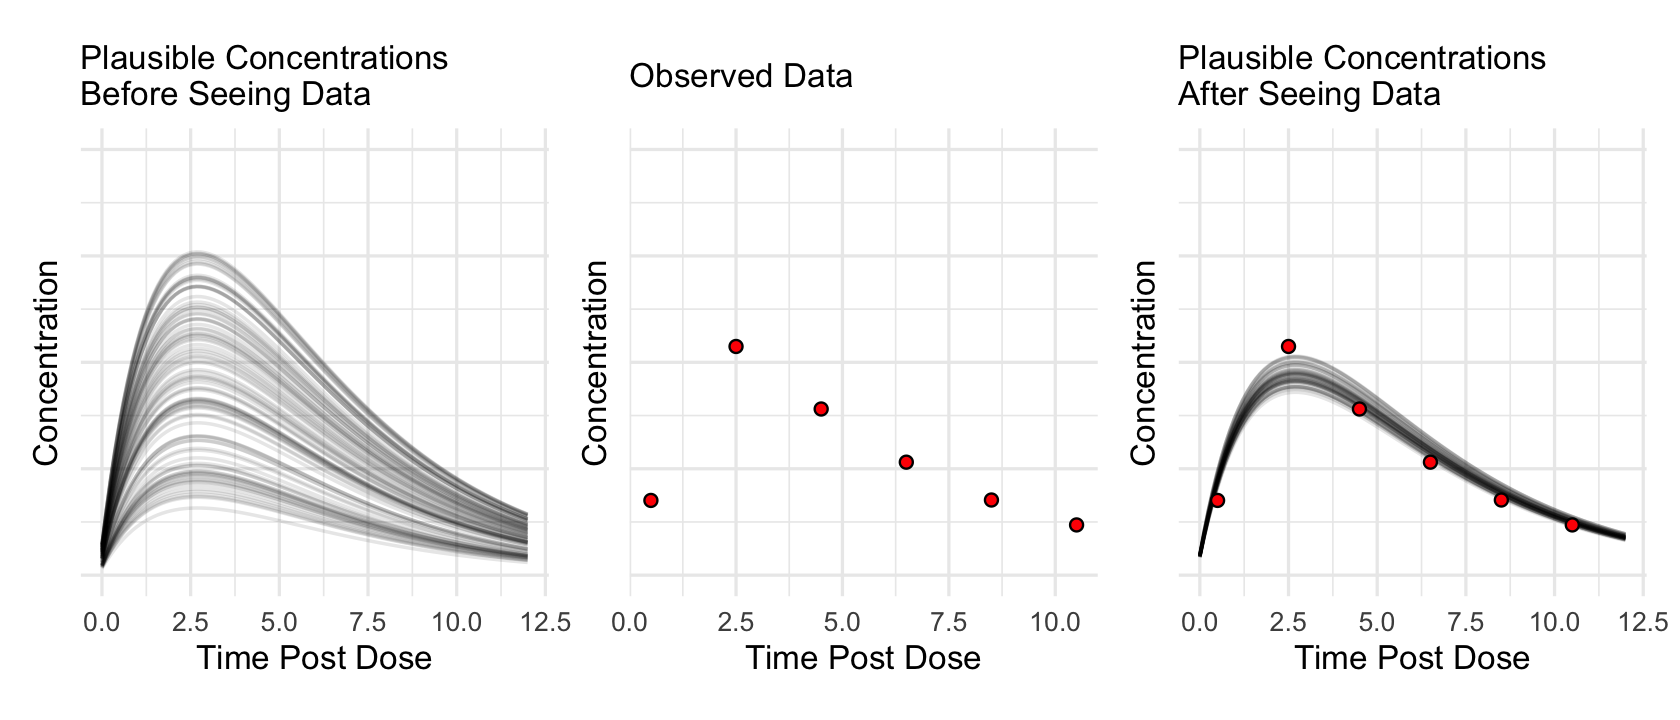
\includegraphics[width=\linewidth]{figures/fig_1}
	\caption{A demonstration of a Bayesian workflow for pharmacokinetic models.  The leftmost panel represents the prior.  Each curve corresponds to a unique set of model parameters which induce each concentration function.  In the center panel is the data observed from a single patient.  Conditioning on this data yields the rightmost panel.  Each curve corresponds to a unique set of model parameters drawn from the posterior distribution.} 
	\label{fig:fig1}
\end{figure}
%
\subsection*{Dosing Decisions}

Vitamin K antagonists, such as the popular oral anticoagulant Warfarin, are known to have narrow therapeutic windows as well as drug and food interaction. Determination of a maintenance dose is consequently a procedure with frequent monitoring and followup, with some sources recommending monitoring daily or every other day until the INR stabilizes for two days.  The narrow therapeutic window forces investigators to also consider the pharmacodynamics (the study of the onset, intensity, and duration of the drug response and how these are related to the concentration of the drug at its site of action) of Warfarin in addition to the pharmacokinetics when determining dose size as concentration of the drug alone is not sufficient to infer the antithrombotic effect in patients. The introduction of factor Xa inhibitors like apixaban has alleviated some of the difficulties in prescribing anticoagulants.  Factor Xa inhibitors have been shown to have lower risk for bleeding than Warfarin in patients with atrial fibrillation \cite{vinogradova2018risks} and also allow for fixed dosing without frequent monitoring of INR. Furthermore, unlike Warfarin, the pharmacodynamic effect of apixaban on clotting is closely correlated with the concentration in the plasma \cite{Byon2019-gf}, making pharmacokinetic modelling more informative on antithrombotic effect as compared to Warfarin.  However, as of writing this paper there is little information on the therapeutic window, making selecting dose sizes large enough to avoid thromboembolism difficult. Furthermore, studies have demonstrated that inter-patient variability of apixaban plasma concentrations is much higher than was initially believed \cite{gulilat2020drug}. In this work, we develop personalized dosing whose goal is to find the  dose that avoids plasma concentrations that are too low too high.


		\section{Methods}

\subsection*{Bayesian Model}

To achieve our three objectives of 1) developing a new Bayesian pharmacokinetic model for apixaban, 2) investigating the impact of MAP versus HMC inference on dosing decisions and 3) developing an induction dosing model for apixaban, we fit a hierarchical mixed effects model of apixaban pharmacokinetics using data from \cite{Beaton2018-el}.  Thirty-six participants were given 2.5 mg of apixaban and 100 ml of water in a fasted state. Blood plasma concentrations of apixaban were recorded over the course of 12 hours.



\begin{table}[htb]
	\centering
	\caption{Summary of data from  \cite{Beaton2018-el} to fit our hierarchical pharmacokinetic model.  Each of the 36 patients was observed 8 times over the course of 12 hours. } 
	\label{tab:my table} 
	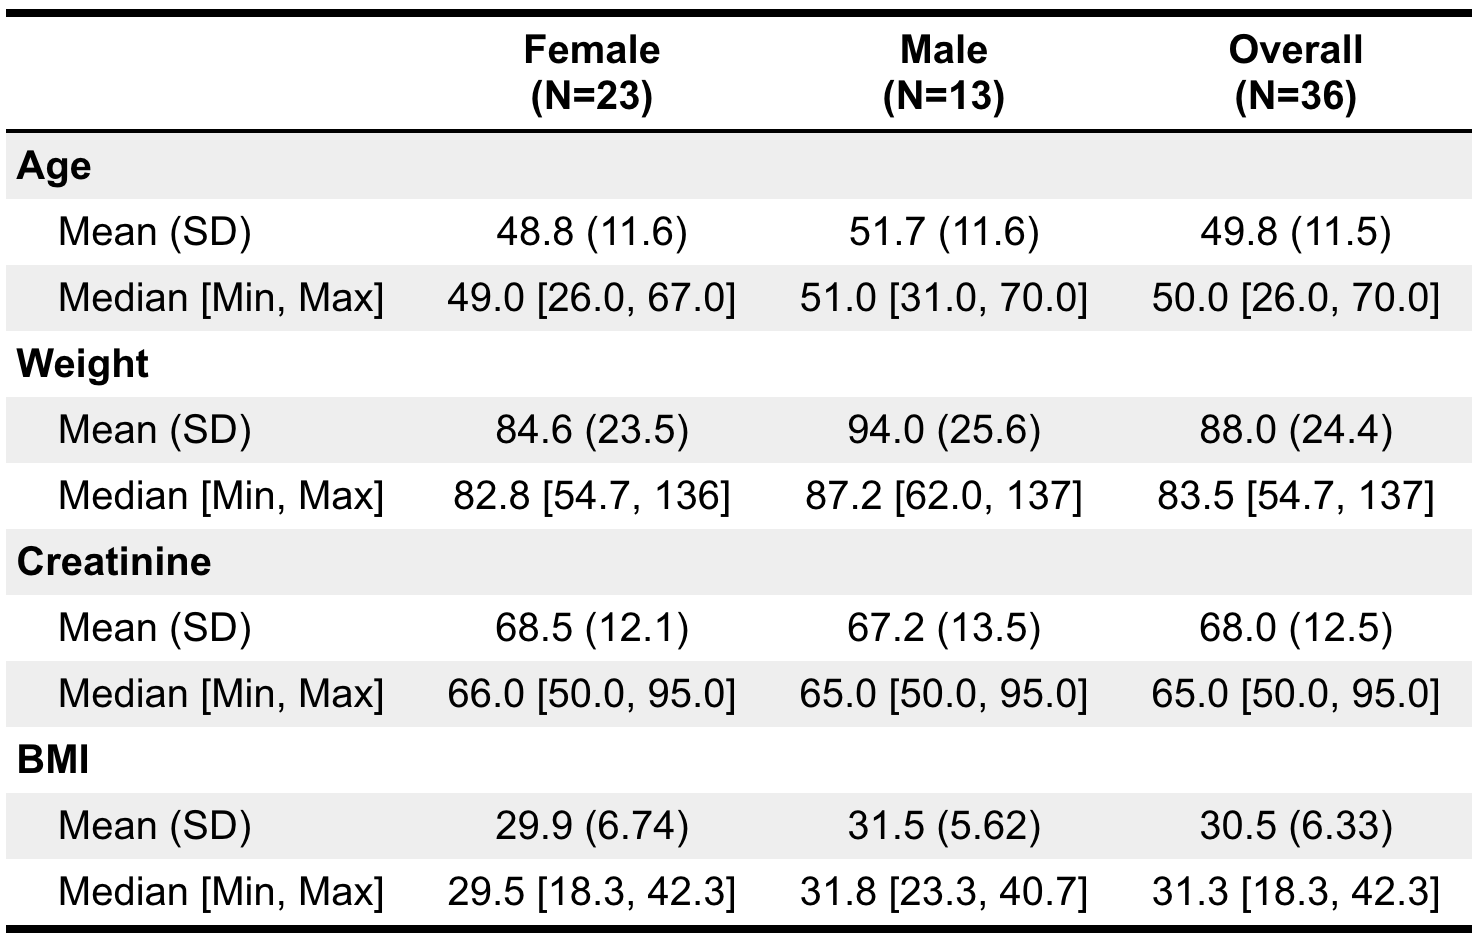
\includegraphics[width=0.7\linewidth]{figures/table1}
\end{table}


\noindent Since participants were given a single dose of apixaban in a fasted state, we use a single-compartment pharmacokinetic model with first order absorption and elimination. The model can be written as a differential equation, namely

\begin{equation}
	\dfrac{dC}{dt} = \dfrac{FDk_ak_e}{Cl}\exp(-k_at) - k_e C(t) \>, C(0) = 0 \>.
\end{equation}

\noindent Here, $D$ is the size of the dose in mg, $F$ is the bioavailability (fixed to 0.5 for apixaban \cite{Byon2019-gf}), $\mathit{Cl}$ is the clearance rate in units litres per hour, $k_a$ is the rate constant of absorption into the volume of distribution in units 1/hours, and $k_e$ is the elimination rate constant in units 1/hours.  The differential equation can be non-dimensionalized by letting $\tau$ and $y(\tau)$ be the non-dimensional quantities, and letting $C(t) = k_ek_a FD y(\tau) / Cl$ and $t = \tau/k_a$.  The non-dimensionalized differential equation is then

\begin{equation}
	\dfrac{dy(\tau)}{d\tau} = \exp(-\tau) - \alpha y(\tau) \>.
\end{equation}


\noindent Here, $\alpha = k_e / k_a$ is the ratio of elimination and absorption rates, and is dimensionless.  The differential equation's qualitative behaviour depends solely on this ratio, with all parameterizations in which $\alpha$ is constant displaying the same qualitative behaviour.  The remaining variables $Cl$, $D$, and $F$ only serve to scale the solution vertically.  The solution to this differential equation (obtained via integrating factors or the Laplace Transform) is

\begin{equation}\label{key}
	y(\tau) = \dfrac{1}{\alpha -1} \Big( \exp(-\tau) - \exp(-\alpha \tau) \Big)
\end{equation}

\noindent After solving the differential equation and converting back to dimensional variables, the solution to the differential equation describing mass transit, and consequently the concentration function, is then

\begin{equation}\label{onecompartment_PKPD}
	C(t) = \dfrac{F D}{Cl}\dfrac{k_ek_a}{k_e - k_a}\Big(e^{-k_at} - e^{-k_et}\Big) \>.
\end{equation}


\begin{figure}[h!]
	\centering
	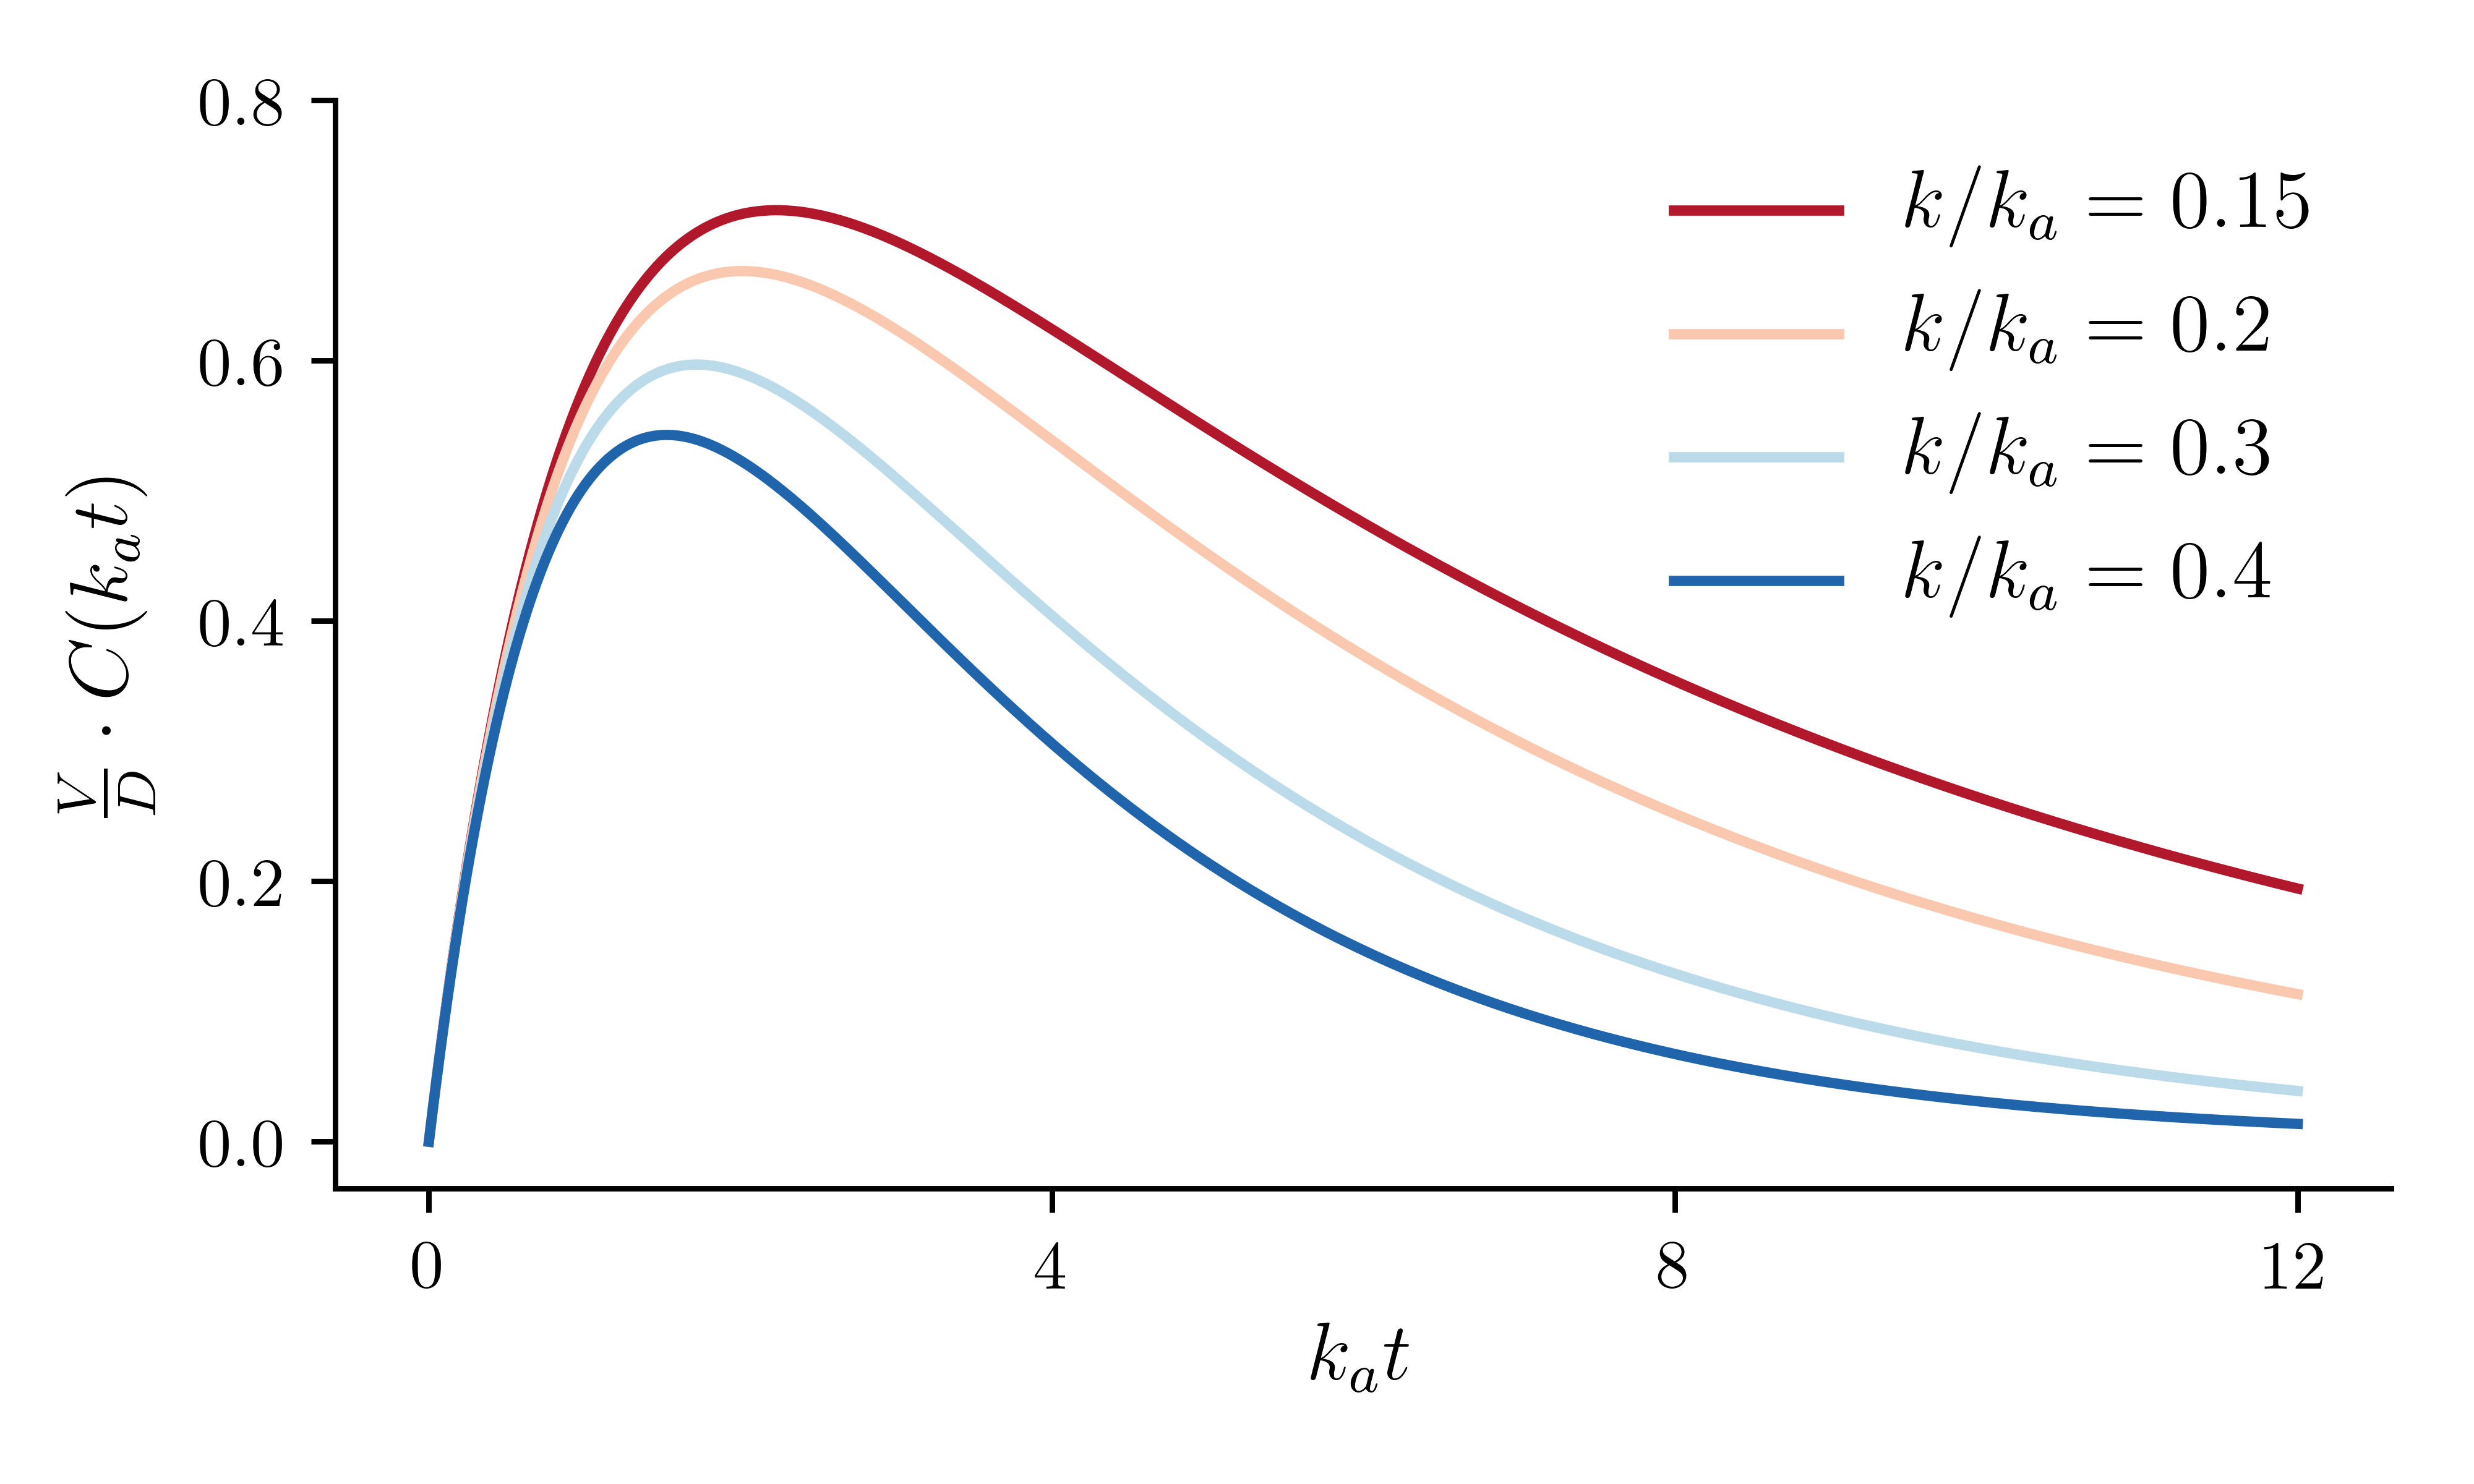
\includegraphics{figures/pkcurves.png}
	\caption[Non-dimensionalized solutions to pharmacokinetic differential equation] {Non-dimensionalized concentration plotted against non-dimensionalized time.  The process non-dimensionalizing the differential equation removes all units from the model, allowing for qualitative comparisons of the solution under different families of parameterization.  Here, it is shown that all parametrizations in which $\alpha = k_e/ka = 0.15$ elicit larger concentrations than those parameterizations in which $\alpha=0.4$ conditioned on $FD/V$ remaining constant.}
	\label{fig:pkcureves}
\end{figure}


For our model, we use a slightly modified version of this function

\begin{equation} \label{eq:eq_1}
C(t) =  \begin{cases}  \dfrac{F \cdot D}{\mathit{Cl}} \dfrac{k_e \cdot k_a}{k_e - k_a}\Bigg( e^{-k_a (t-\delta)} - e^{-k_e(t-\delta)} \Bigg)  & \delta \leq t\\\\ 0 & \mbox{else} \end{cases}
\end{equation}

\noindent We include a time delay, $\delta$, to relax the assumption that absorption begins immediately after ingestion.  Parameters are modelled using random effects, with some population mean and variance (which is estimated from the data). 

Priors for $k_e$ and $k_a$ are not defined explicitly.  Rather, our model puts priors on the time to maximum concentration, which can be expressed as a function of the parameters in \cref{eq:eq_1}

\begin{equation}\label{eq:eq_2}
 t_{\mathit{max}} = \dfrac{\ln(k_a) - \ln(k_e)}{k_a - k_e}
\end{equation}

\noindent and on the ratio between $k_e$ and $k_a$, which we call $\alpha$

\begin{equation}\label{eq:eq_3}
\alpha  = \dfrac{k_e}{k_a} \>.
\end{equation}

\noindent We choose to place a prior on the quantity $\alpha$ because it arises when non-dimensionalizing \cite{holmes2009introduction} the differential equation governing mass transit of the drug in and out of the volume of distribution.  The plasma concentration function is a version of the “flip-flop” model \cite{Wakefield1996-yy, Salway2008-gi}, since different parameterizations of this model can yield the same curve, leading to model un-identifiability. To ensure the model is identifiable, we require $k_e<k_a$ as has been done in previous Bayesian analyses of this model \cite{Wakefield1996-yy, Salway2008-gi}. This requirement bounds $\alpha$ to the unit interval. Using a standard parameterization of the model (in terms of $k_e$ and $k_a$) resulted in poor sampling behaviour as indicated by the sampling diagnostics.  In particular, because of an unenforceable constraint that $k_e < k_a$ or $k_a < k_e$, the model suffered from poor mixing as indicated by the Gelman-Rubin diagnostic $\hat{R}$. Wakefield approached the problem of identifiability by \cite{wakefield1992bayesian} by placing priors on $k_a$, and $V$ (the volume of distribution for the drug) and $Cl$ for patients separately, (thereby allowing him to solve for $k_e$), however there was insufficient prior information on $k_a$ and $V$ for apixaban.
Placing a relatively non-informative prior determined through prior predictive checks on $\alpha$ and using the estimate of time to maximum concentration ($t_{\max}$, for which there was prior information) allowed us to solve for either $k_e$ or $k_a$ and then use the relationship $\alpha = k_e / k_a$ to solve for the remaining rate constant.  This rectified the poor mixing behaviour and facilitated sampling with HMC.  In principle, information on the elimination rate constant could be obtained by performing a linear regression on the log concentration values in the latter half of the concentration profiles where the drug is being eliminated from the body. To preserve as much data as possible for model fitting, we forgo this approach.  These two sets of equations are used to parameterize the absorption and elimination rate constants as follows
\begin{align}
	k_a &= \dfrac{1}{t_{\mathit{max}}} \dfrac{\ln(\alpha)}{\alpha-1} \label{eq:eq_4} \\
	k_e &= k_a \alpha \label{eq:eq_5}
\end{align}

%Time to max concentration values for patient $j$ are drawn from a log normal distribution
%
%\begin{equation}\label{eq:eq_6}
%t_{\mathit{max}, j} \vert \mu_t, \sigma_t \sim \operatorname{LogNormal}(\mu_t, \sigma_t)
%\end{equation}
%
%\noindent and $\alpha$ is drawn from a weakly informative beta prior to prevent degenerate cases when $\alpha$  is 0 or 1
%
%\begin{equation}\label{eq:eq_7}
%\alpha_j \sim \operatorname{Beta}(2,2)  \>.
%\end{equation}
%
%\noindent The rate constants for patient $j$,  $k_{e,j}$ and $k_{a,j}$, are determined from \cref{eq:eq_4,eq:eq_5}. The clearance rate is modelled hierarchically
%
%\begin{equation}\label{eq:eq_8}
%\mathit{Cl}_j \vert \mu_{\mathit{Cl}}, \sigma_{\mathit{Cl}}  \sim \operatorname{LogNormal}(\mu_{\mathit{Cl}}, \sigma_{\mathit{Cl}}) \>.
%\end{equation}
%
%\noindent Each patient is observed to have a non-zero concentration at time 0.5, so the time delay for each patient is no larger than 0.5 hours.  We place a beta prior on the delay
%
%\begin{equation}\label{eq:eq_9}
%\delta_j \vert \phi, \kappa \sim \operatorname{Beta}(\phi / \kappa, (1-\phi) / \kappa)
%\end{equation}
%
%\noindent and multiply delta by 0.5 in our model to ensure the maximum delay is 0.5 hours.  Here, $\phi$ is the mean of this beta distribution and $\kappa$ determines the precision of the distribution. Shown in \cref{net} is a Bayes net to exposit model structure at a high level.
%
%\begin{figure}[h!]
%	\centering
%	\begin{tikzpicture}
%	
%	\node[latent](phi){$\phi$};
%	\node[latent, right=of phi](kappa){$\kappa$};
%	\node[latent, right = of kappa](s_t){$\sigma_t$};
%	\node[latent, right = of s_t](m_t){$\mu_t$};
%	\node[latent, right = of m_t](s_cl){$\sigma_{\mathit{Cl}}$};
%	\node[latent, right = of s_cl](m_cl){$\mu_{\mathit{Cl}}$};
%	
%	\node[latent, below = of kappa](delta){$\delta$};
%	\node[latent, right = of delta](alpha){$\alpha$};
%	\node[latent, below = of m_t](tmax){$t_{\mathit{max}}$};
%	\node[latent, below = of s_cl](cl){$\mathit{Cl}$};
%	
%	\node[obs, below = of alpha](t){$t$};
%	\node[obs, right = of t](y){$y$};
%	\node[latent, right = of t, xshift = 3.25cm](sig){$\sigma_y$};
%	
%	\edge{phi}{delta};
%	\edge{kappa}{delta};
%	
%	\edge{s_t}{tmax};
%	\edge{m_t}{tmax};
%	\edge{s_cl}{cl};
%	\edge{m_cl}{cl};
%	
%	\edge{delta}{y};
%	\edge{alpha}{y};
%	\edge{tmax}{y};
%	\edge{cl}{y};
%	\edge{t}{y};
%	\edge{sig}{y};
%	
%	\plate{t_y_pairs}{(t)(y)}{$i=1\dots 8$};
%	\plate{patient_level}{(t_y_pairs)(delta)(alpha)(tmax)(cl)}{$j = 1 \dots 36$};
%	\end{tikzpicture}
%	
%	
%	\caption{Graphical description of the data generating process for our model.  The data consist of 36 patients, indexed by $j$.  Each of the $j$ patients are observed a total of 8 times, with each observation index by $i$.  The data are generated by drawing random variables from their appropriate distribution at the top level and then drawing child random variables directly there after.  As an example, $\phi$ and $\kappa$ are drawn, which are then used to draw the $\delta_j$, which are then used to draw each of the 8 concentration values, $y_i$ for each of the $j$ patients.}
%	\label{net}
%\end{figure}
%
%\subsection*{Priors for Model Hyperparameters}
%
%Estimates of the time to max concentration for apixaban place the population median $t_{\mathit{max}}$ near 3.3 hours post dose  \cite{Byon2019-gf}. Assuming the median and the mean are similar, this provides information for $\mu_t$ and so we use specify 
%
%\begin{equation}\label{eq:eq_10}
% p(\mu_t) = \operatorname{Normal}(\log(3.3), 0.25)
%\end{equation}
%
%\noindent The standard deviation of the prior for $\mu_t$ was selected via prior predictive checks in which profiles are drawn and priors are assessed as realistic or not.  We choose to err on the side of caution and inflate the uncertainty in this estimate to account for population differences between the measured patients in the data and the patients used in studies to determine the estimates of $t_{\mathit{max}}$. The population variability of $t_{\mathit{max}}$ was modeled as
%
%\begin{equation}\label{eq:eq_11}
%p(\sigma_t) = \operatorname{Gamma}(10,100)
%\end{equation}
%
%\noindent Using these priors, we recover similar median, min, and max $t_{\mathit{max}}$ values as reported by \cite{Byon2019-gf}. Similarly, we model the population mean and variability for the clearance rate as
%
%\begin{align}
%	p(\mu_{\mathit{Cl}}) &= \operatorname{Normal}(\log(3.3), 0.15) \label{eq:eq_12} \\
%	p(\sigma_{\mathit{Cl}}) &= \operatorname{Gamma}(15, 100) \label{eq:eq_13}
%\end{align}
%
%\noindent so that population estimates of the mean clearance rate are near 3.3 litres per hour with inflated uncertainty to account for possible population differences. We use weakly informative priors for $\phi$ and $\kappa$ which induces an approximately uniform prior on $\delta$.
%
%\begin{align}
%	 p(\phi) &= \operatorname{Beta}(20,20) \label{eq:eq_14}\\
%	 p(\kappa) &= \operatorname{Beta}(20,20)  \label{eq:eq_15}
%\end{align}
%
%The tools used to measure the concentration of apixaban are believed to be within 10\% of the real concentration.  This implies that the observational model is heteroskedastic. We use a log-normal likelihood so that positivity of observed concentrations and heteroskedasticity are respected. We place a lognormal prior on the likelihood’s variability with
%
%\begin{align}
%	p(\sigma_y)  &= \operatorname{LogNormal}(\ln(0.1), 0.2) \label{eq:eq_16}\\
%	C_{j}(t) \vert \mathit{Cl}_{j}, k_{a,j}, k_{a,j}, \delta_j &\sim \operatorname{LogNormal}(\ln(y(t)), \sigma_y)  \label{eq:eq_17}
%\end{align}

Details on the prior distributions for each parameter and the model likelihood can be found in the appendix.  We also include a summary of the model's posterior as well as details on simulating data from the model's posterior predictive distribution to generate pseudopatients for use in our experiments.

\subsection*{Model Fitting and Diagnostics}

For HMC, prior/posterior predictive checks and model fitting was performed using Stan \cite{Carpenter2017-qf} to draw from the prior/posterior.  Twelve chains were initialized and run for 4000 iterations each (1000 for warmup allowing the Markov chain the opportunity to find the correct target distribution and 3000 to use as samples from the posterior). Stan monitors several diagnostics none of which detected problematic HMC behavior\footnote{0 divergences, all Gelman-Rubin diagnostics $<1.01$, smallest effective sample size ratio 16\%.}.

We use Stan’s optimization capabilities to compute the MAP estimates.  The L-BFGS optimizer was used to find the posterior mode.  The optimizer terminated when either 10,000 iterations had been performed or when the value of the objective function stopped changing within a tolerance of $1\times10^{-10}$. Once the mode was located, 10,000 samples from the Laplace approximation to the posterior were obtained. Constrained parameters were transformed to the appropriate space before sampling.

%\subsection*{Posterior Summarization and Generating New Data}
%
%Once our model was fit on the pharmacokinetic data, the marginal posteriors were summarized to create priors for the new model.  Parameters for these priors were determined by using maximum likelihood on the posterior samples.  The priors for the new model are as follows:
%
%\begin{align}
%	\mu_{\mathit{Cl}} &\sim \operatorname{Normal}(1.64, 0.09)  \label{eq:eq_18} \\
%	\sigma_{\mathit{Cl}} &\sim \operatorname{LogNormal}(-0.94, 0.11)  \label{eq:eq_19} \\
%	\mu_{t} &\sim \operatorname{Normal}(0.97, 0.05)   \label{eq:eq_20} \\
%	\sigma_{t} &\sim \operatorname{LogNormal}(-1.40, 0.12)  \label{eq:eq_21} \\
%	\alpha_j &\sim \operatorname{Beta}(2,2)  \label{eq:eq_22} \\
%	\sigma_y &\sim \operatorname{LogNormal}(-1.76, 0.12)  \label{eq:eq_23}
%\end{align}
%
%\noindent Lognormal distributions were used to respect positivity of some parameters.  The posterior predictive distribution of the model fit to the data from \cite{Byon2019-gf} was then used to simulate 100  pseudopatients.  The time delay, $\delta$ was not used to generate these data as $\delta$ does not affect the overall shape of the concentration function, it merely shifts if right.  The model with the priors defined by \crefrange{eq:eq_18}{eq:eq_23} was then refit on the 100  pseudopatients in order to examine differences between HMC and MAP in a “best case” scenario. The pseudopatients were sampled between 0.5 and 12.0 hours after ingestion in increments of 0.5. Draws from the posterior were used to predict latent concentration for each patient at times 0.75 to 11.75 in increments of 0.5.

\subsection*{Determination of a Personalized Dose}

The results from both  HMC and MAP yield samples from the approximate posterior of $\mathit{Cl}_{j}$, $k_{e,j}$, $k_{a,j}$, and $\delta_j$ for each of the $j$ patients.  For any given posterior sample, these parameters can be combined to compute a predicted concentration for patient $j$ at time $t$ by using \cref{eq:eq_1}.   We determine a personalized dose size by evaluating the pseudopatients’ concentration function under different dose sizes $D$ and then computing posterior probabilities of failing to surpass concentration thresholds.  When we have posterior samples, \cref{eq:eq_1} turns into a function of the dose size and time conditioned on patient. 


We perform two experiments to compare HMC and MAP.  In our first experiment, we determine the posterior probability of failing to exceed a concentration of 20 ng/ml 12 hours post dose for each pseudopatient across a variety of dose sizes. We choose 20 ng/ml as our threshold for this experiment because the median concentration at 12 hours post dose  in the data from \cite{Beaton2018-el} is approximately 20 ng/ml. In our second experiment, we determine the posterior probability that the maximum concentration fails to exceed 80 ng/ml.  We choose 80 ng/ml as our threshold for this experiment because the median maximum concentration in the data is 79 ng/ml (though it is important to note that it is unlikely that these patients were observed exactly at the time which the peak concentration was achieved).  These quantities represent two different ways of assessing a patient's risk of being below a given threshold.  The chosen threshold is arbitrary, but our method generalizes to any threshold.  For each experiment, the risks are computed across a grid of dose sizes of 0 mg to 60 mg, yielding risk as a function of dose size.  For each pseudopatient, we interpolate these estimates using a monotone Hermite spline and then invert the risk curve; the inverted risk curve maps risk to dose. This allows us to determine a dose size which produces a specified risk level.



		\section{Results}
\subsection*{Bayesian Model}

Diagnostic plots for our Bayesian model fot to the real apixaban data are shown in \cref{fig:fig3}.  Posterior population prediction intervals (that is, the result of integrating out the random effect of each patient) of the observed concentration are realistic and to the eye appear similar to the observed data (top left of \cref{fig:fig3}).  Residual plots (observed minus posterior mean) indicate homogeneity of variance on the log scale, which is consistent both with expert knowledge on the measurement process and the likelihood we choose (bottom left of \cref{fig:fig3}). Predicted concentrations tend to agree with observed concentrations (top right of \cref{fig:fig3}), and posterior predictive draws have similar empirical cumulative distribution functions as the observed data (bottom right of \cref{fig:fig3} ). In \cref{fig:fig4}, we show concentration functions obtained from draws from our prior distribution as well as two patients with best and worst fit as measured by mean absolute percentage error (best: 3.29\%, worst: 26.4\%). Because our HMC diagnostics do not indicate problematic behaviour in the Markov chains, and because the model diagnostics indicate adequate fit, we believe the obtained model’s posterior predictive distribution is adequate for simulation of pseudopatients.


\begin{figure}
	\centering
	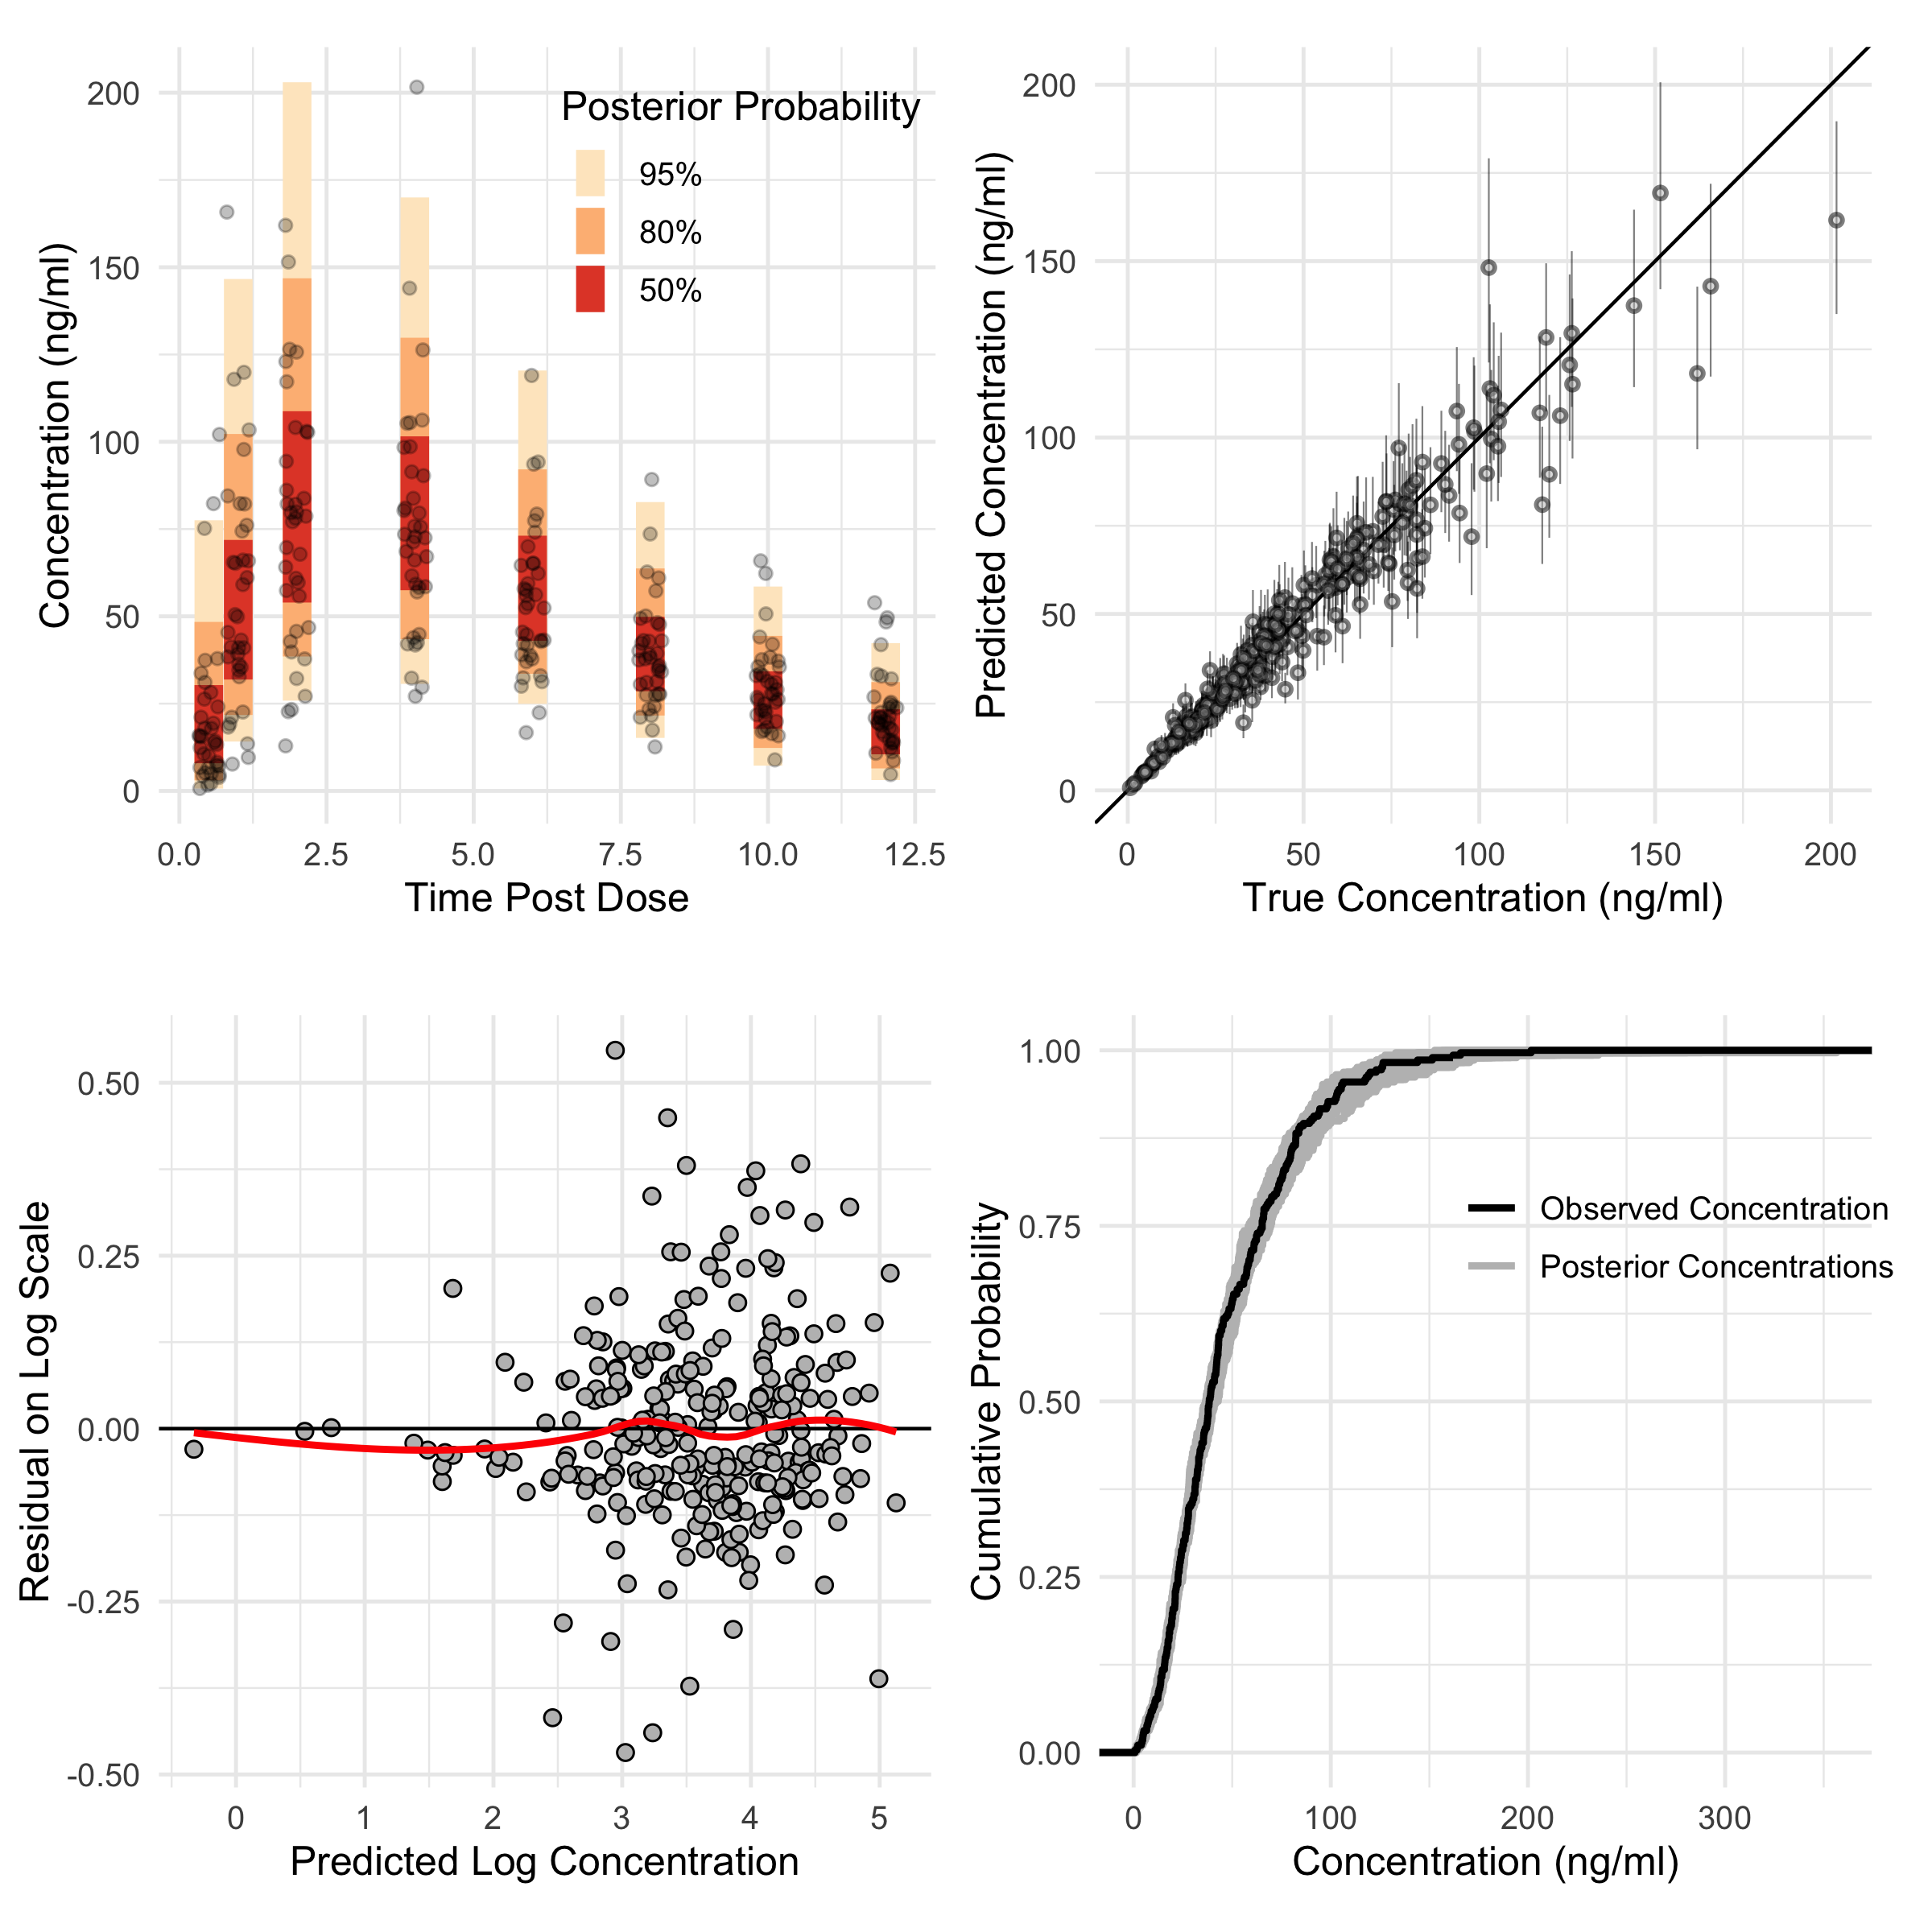
\includegraphics[width=0.9\linewidth]{figures/diagnostics}
	\caption{Diagnostic plots for our Bayesian model fit to the real data.  Top left shows the posterior predictive distribution plus observed data.  Data points gave been perturbed to prevent overlapping. Top right shows the predicted values along with accompanying 95\% equal-tailed posterior credible interval. Bottom left shows the residuals (on the log scale) between the observed concentrations and the posterior mean concentration, bottom right shows the cumulative density function for the observed data (black) as well as draws from the posterior predictive distribution (gray).}
	\label{fig:fig3}
\end{figure}


\begin{figure}
	\centering
	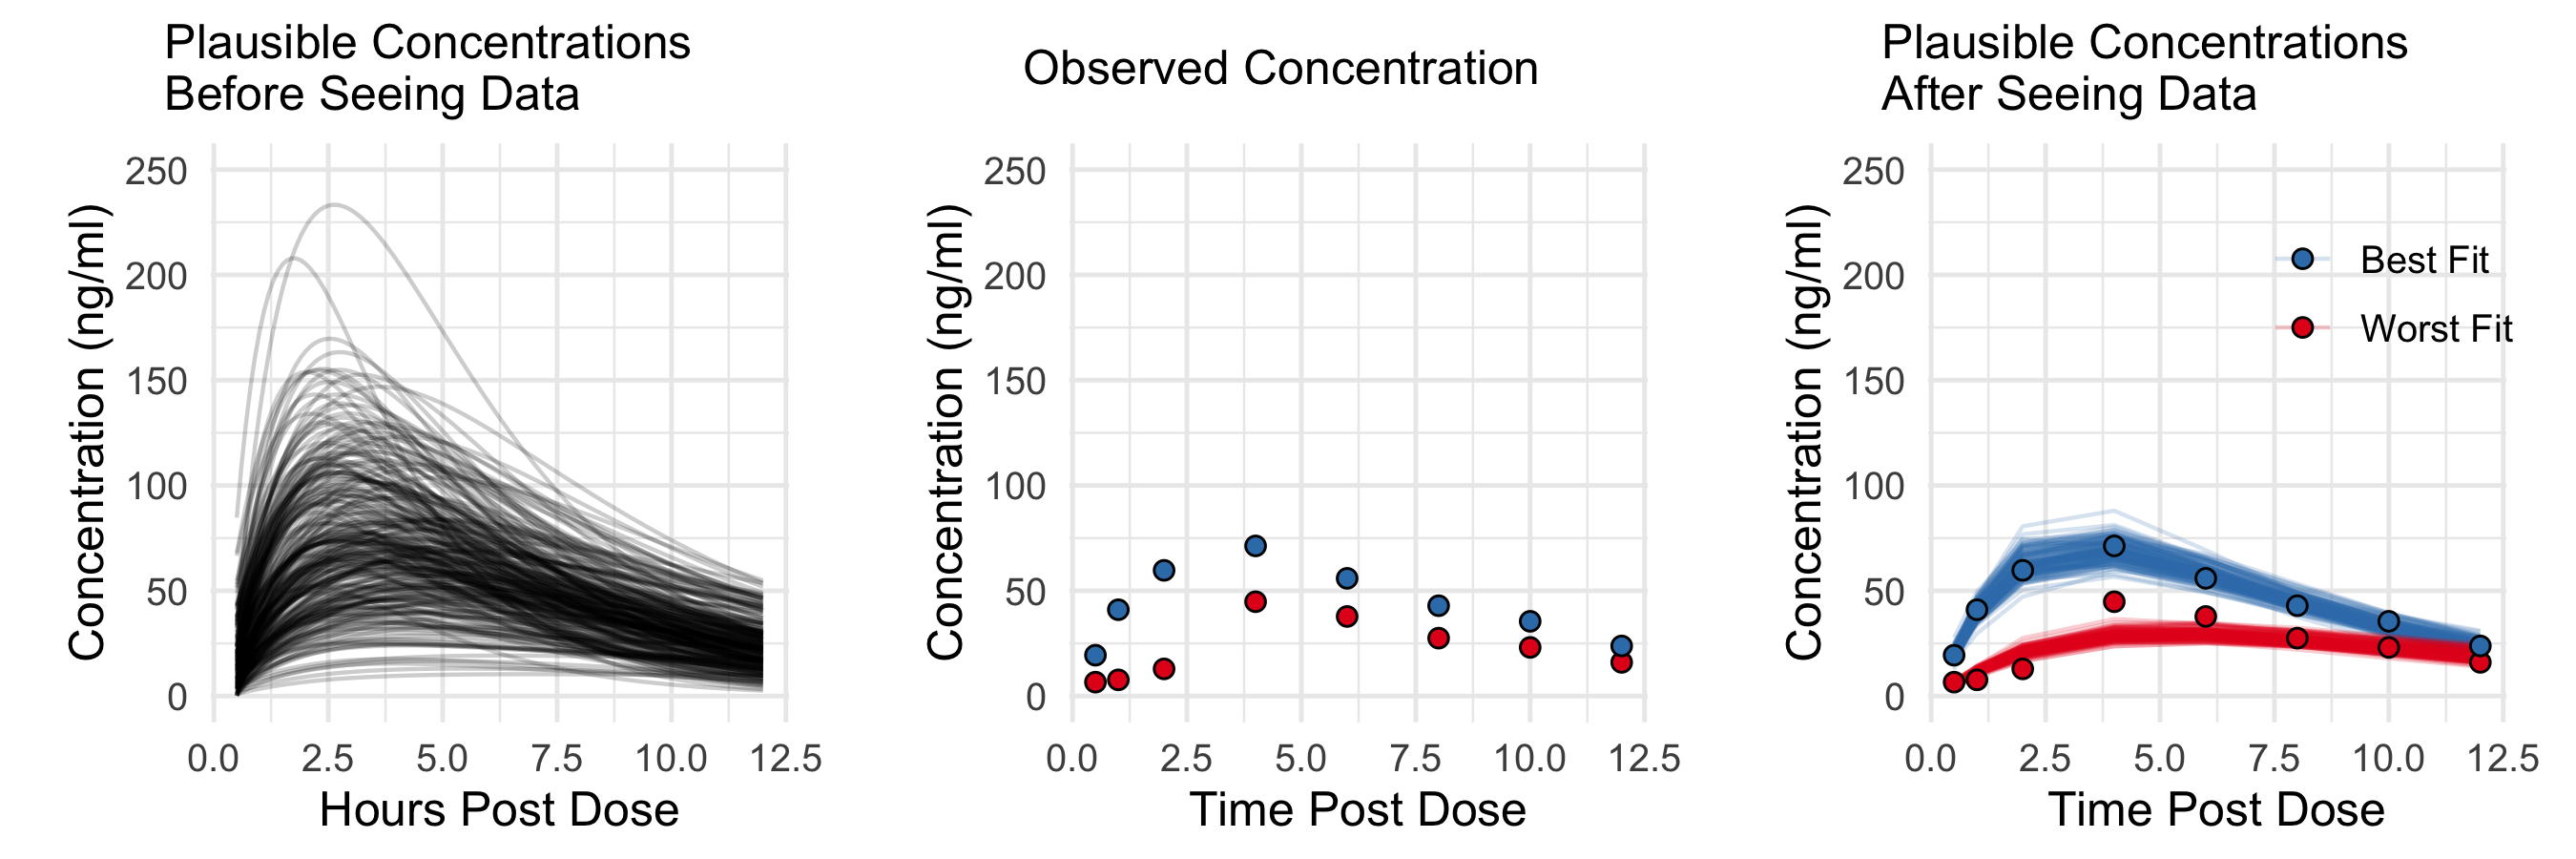
\includegraphics[width=\linewidth]{figures/fig3}
	\caption{The leftmost panel shows 250 draws from the prior defined in the previous section.  The center panel shows data from two patients who achieved the best (blue) and worst (red) model fit as measured through mean absolute percent error.  The rightmost panel shows 250 draws from the posterior for these patients.  Not shown here are the other 34 patients in our data, for which the model is also capable of performing predictions for. }
	\label{fig:fig4}
\end{figure}

%\begin{figure}
%	\centering
%	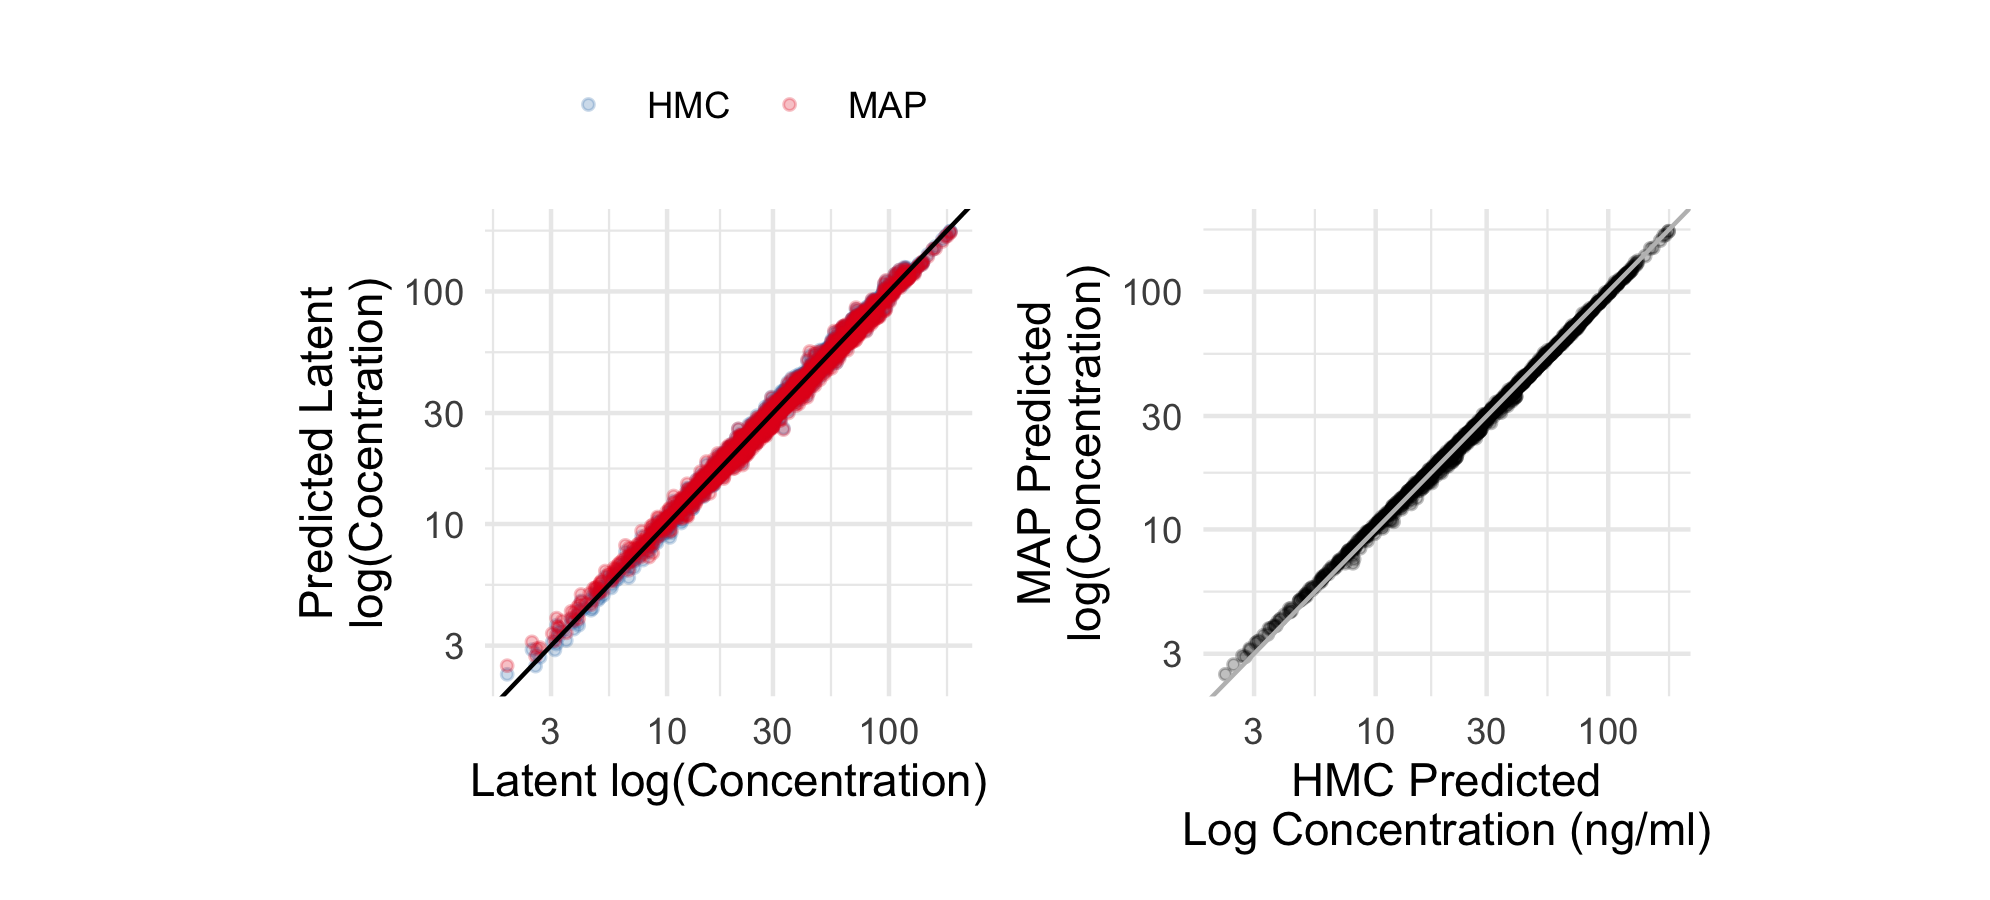
\includegraphics[width=1\linewidth]{figs/compare}
%	\caption{Comparisons of fits obtained through HMC and MAP for simulated patients.  On the left, the two methods are compared to the true concentration values, and on the right the two methods are compared to one another.  The predictions are negligibly different to the eye and are also negligibly different as compared by Mean Squared Error (MSE), Mean Absolute Error (MAE), and Mean Absolute Percentage Error (MAPE).}
%	\label{fig:fig5}
%\end{figure}



\subsection*{Fit on Simulated Patients Using HMC and MAP}

Initial comparisons of predicted values indicate that both HMC and MAP yield similar predictions to one another, and similar predictions to actual values of unseen data.  Examining predictions alone, it would seem that HMC and MAP are equivalent, or at the very least similar enough so as to not have strong preference for one over the other. When using posterior means, HMC results in lower prediction error on unseen data (see \cref{table2}) as measured with Mean Squared Error (MSE), Mean Absolute Error (MAE), and Mean Absolute Percentage Error (MAPE), but these are not stark differences. Estimates of posterior uncertainty between MAP and HMC can however vary a great deal. Shown in \cref{fig:fig6} are 19 of the 100 simulated patients which have a MAP equal tailed posterior interval at least 50\% larger as compared to their HMC equal tail posterior interval at the widest point. We note that while not shown explicitly, unobserved concentrations lie entirely within the HMC and MAP posterior intervals.



\begin{table}
	\centering
\begin{tabular}{|c|c|c|}
	\hline 
	& HMC & MAP \\ 
	\hline 
	MSE (SD) & 6.67 (15.93) & 8.57 (19.93) \\ 
	\hline 
	MAE (SD) & 1.71 (1.94) & 1.97 (2.17) \\ 
	\hline 
	MAPE (SD) & 0.04 (0.03) & 0.05 (0.03)\\ 
	\hline 
\end{tabular} 
\caption{Comparison of HMC and MAP on three loss functions common in pharmacokinetics:  Mean Squared Error (MSE), Mean Absolute Error (MAE), and Mean Absolute Percentage Error (MAPE).  The loss was computed on samples not seen by our model.  Included in parentheses are the standard deviations of the loss values.}
\label{table2}
\end{table}

%\begin{figure}
%	\centering
%	\includegraphics[width=1\linewidth]{figs/intervals}
%	\caption{Comparisons of equal tail posterior intervals from MAP and HMC. Note that the concentration scales differ from subplot to subplot.  Selected patients are those which have a MAP posterior interval at least 50\% as wide or wider than their HMC interval.  In many simulated subjects.}
%	\label{fig:fig6}
%\end{figure}
\clearpage
\begin{sidewaysfigure}[h!]
\centering
	\includegraphics[width=1\linewidth]{figures/intervals}
	\caption{Comparisons of equal tail posterior intervals from MAP and HMC. Note that the concentration scales differ from subplot to subplot.  Selected patients are those which have a MAP posterior interval at least 50\% as wide or wider than their HMC interval.}
	\label{fig:fig6}
\end{sidewaysfigure}
\clearpage

\subsection*{Difference in Estimated Dose To Achieve Target Risk}

Using the posterior for each pseudopatient, we can determine the risk of exceeding the threshold by varying the dose.  This results in a risk curve which gives risk as a function of dose.  By inverting the risk curve, we can obtain dose size as a function of risk.  Shown in \cref{fig:fig7} are the differences between doses computed from HMC and MAP posteriors to achieve the indicated level of risk.  The left panel shows the difference in doses in order to achieve a concentration of at least 20 ng/ml 12 hours post dose. For a majority of patients, MAP and HMC agree to within 1 mg though some pseudopatients see a much larger dose recommendation by HMC than by MAP.  The right panel shows the difference in doses in order to achieve a max concentration of 80 ng/ml.  MAP tends to always recommend larger doses than HMC for this scenario, with the difference between recommended doses becoming larger as the desired risk becomes smaller.

\begin{figure}[h!]
	\centering
	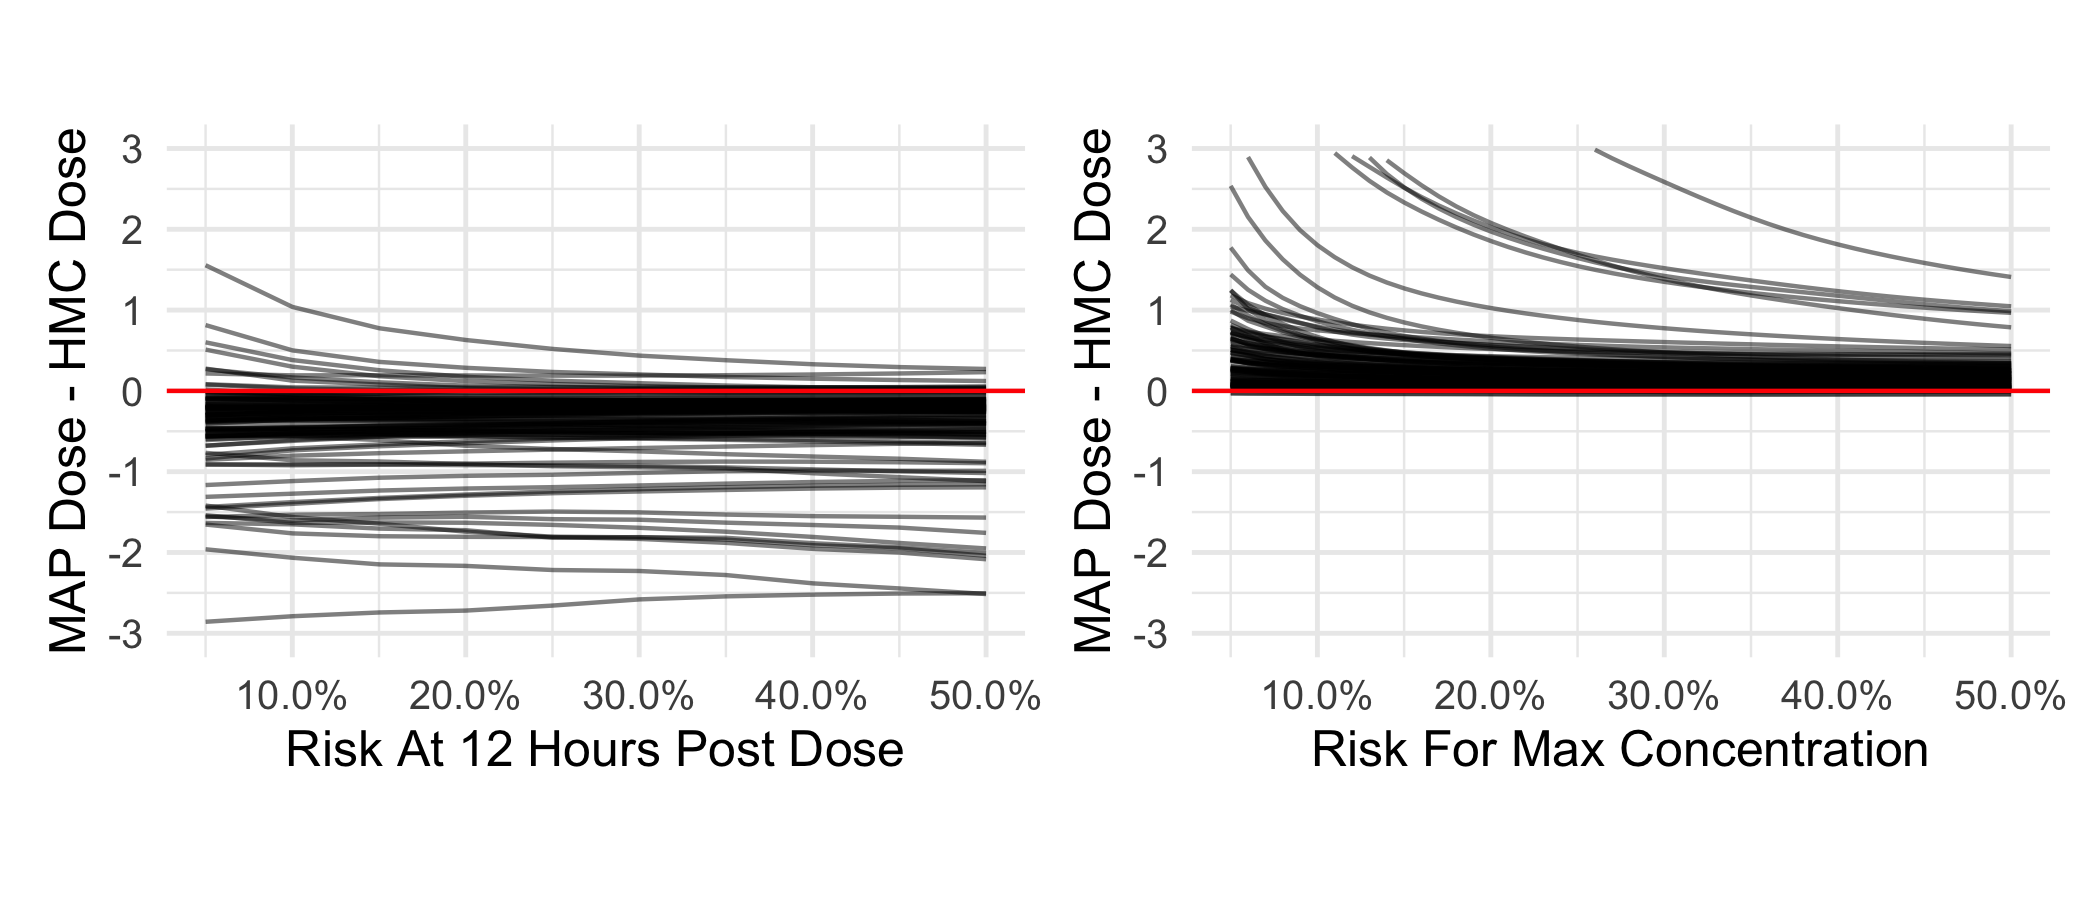
\includegraphics[width=\linewidth]{figures/experiments}
	\caption{Left: Differences between the estimated doses from MAP and HMC to achieve the indicated risk of having a concentration of apixiban smaller than 20 ng/ml at 12 hours post dose. Each line corresponds to one of the 100 pseudopatients. HMC tends to recommend larger doses than MAP to achieve a desired risk of having the patient's concentration at 12 hours post dose be below 20 ng/ml. This tendency to recommend larger doses is consistent across desired risk levels.  Right: Differences between estimated doses from MAP and HMC to achieve the indicated risk of having a max concentration smaller than 80 ng/ml.  Some pseudopatients see dose recommendation differences as large as 10 mg and are thus cut off by the y axis limits. Red lines indicate where the two methods would perfectly agree.}
	\label{fig:fig7}
\end{figure}


\subsection*{Calibration for Dosing Decisions}

Since all pseudopatients were simulated, the true concentration function as a function of the dose size (\cref{eq:eq_1}) was known.  To further compare HMC and MAP for decision making, we took estimated dose size to achieve a desired risk and computed what the concentration curve under the recommended dose size.  We could then compute the number of pseudopatients which actually exceeded the threshold, thus allowing us to examine the calibration of HMC and MAP.  The calibration curves for HMC and MAP for both experiments are shown in \cref{fig:fig8}.

In the first experiment (left of \cref{fig:fig8}), HMC is better calibrated than MAP.  This means that when a dose is selected, in order to a achieve a risk of being below 20 ng/ml at 12 hours post dose of $r$, approximately $r \times 100$ pseudopatients have a true concentration function which is smaller than 20 ng/ml at 12 hours post dose. In contrast, MAP is poorly calibrated, and sees more pseudopatients failing to exceed the 20 ng/ml threshold than was desired.  Calibration in our second experiment again shows than HMC is better calibrated than MAP, but calibration seems to become worse as the desired risk becomes larger.  When we use dose sizes recommended by MAP to achieve a 50\% probability of exceeding the 80 ng/ml threshold, only 26\% of pseudopatients actually have a max concentration which exceeds the threshold.


\begin{figure}[h!]
	\centering
	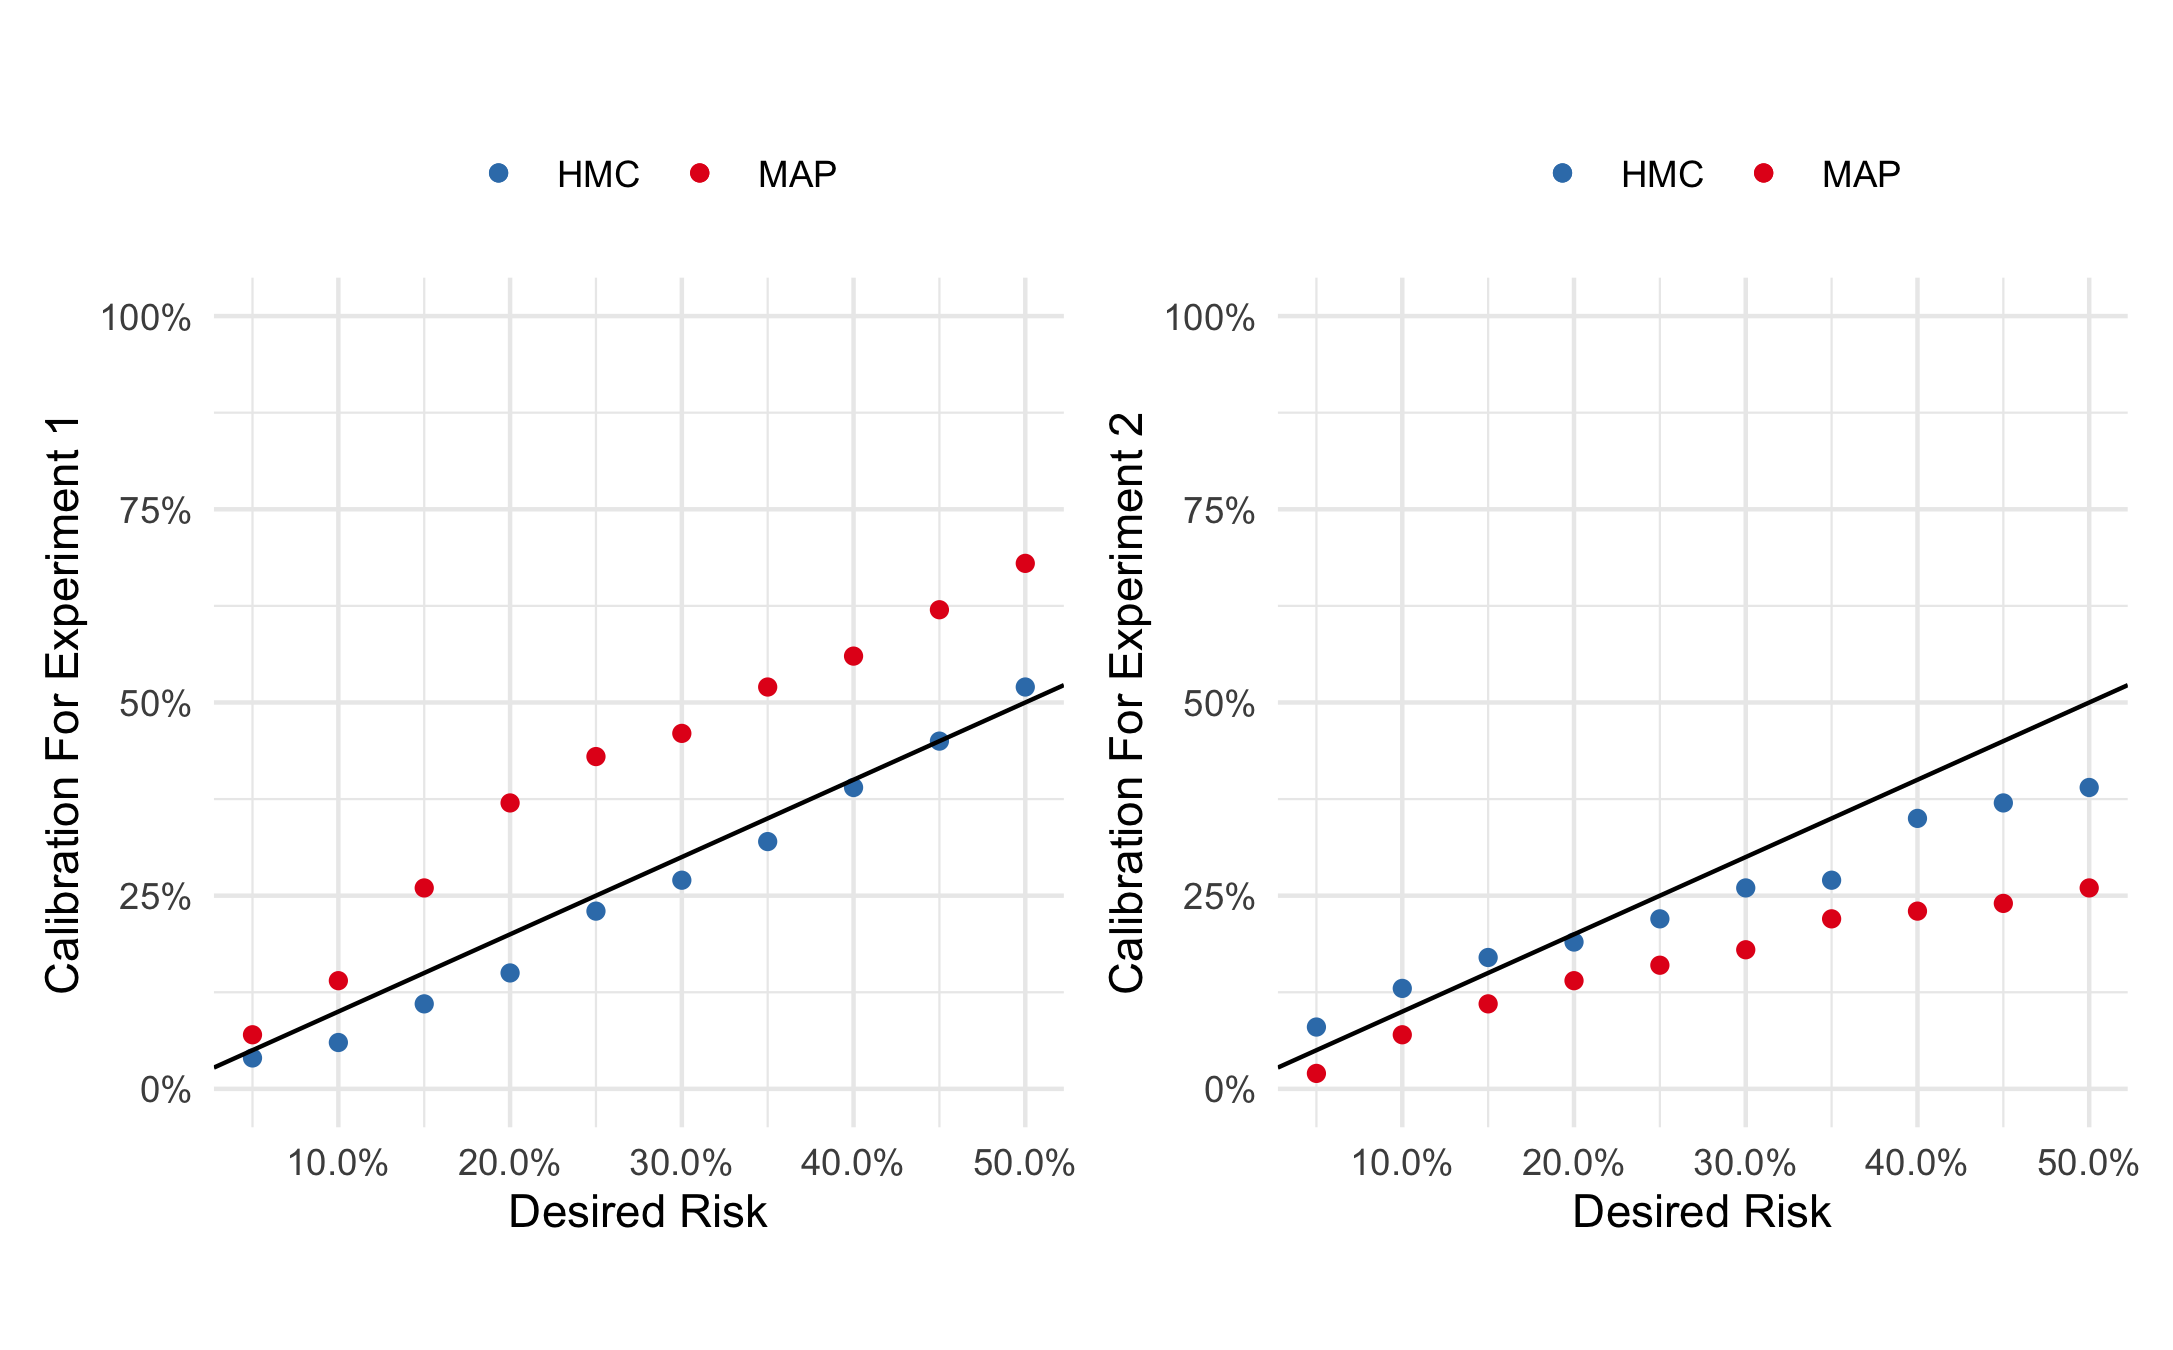
\includegraphics[width=\linewidth]{figures/fig8.png}
	\caption{Left: Calibration curves for assessing risk of being below 20 ng/ml.  Each dot represents the proportion of the 100 pseudopatients which fail to exceed the 20 ng/ml threshold.  When doses are chosen from samples obtained via HMC, then probabilities are well calibrated. When doses are chosen from samples obtained via MAP, more pseudopatients fail to exceed the threshold than were specified.  Right: Calibration curves for assessing risk of the max concentration being below 80 ng/ml. HMC appears to be better calibrated than MAP, though the calibration could stand to improve.}
	\label{fig:fig8}
\end{figure}




		\section{Discussion}

While prediction errors of the point estimates produced by MAP and HMC are very similar as measured by 3 losses common to pharmacokinetic research, they each produce very different estimates of uncertainty.  Such estimates are necessary for decision making under uncertainty, where an expected loss is computed over a posterior distribution.  In this study, for a given dose, MAP assigns a significant amount of probability mass to concentrations which are far lower than the concentrations considered plausible by HMC.  The extent to which this discrepancy would change decisions depends on the loss function, but we see substantial differences in our two example experiments for personalized dosing.  The difference in uncertainty between MAP and HMC results in small disagreement for dose size for the majority of patients, but very large disagreement for a sizable minority of about 20\%. The observed difference in uncertainty for the concentration function between MAP and HMC are likely due to discrepancies in uncertainty over the individual PK parameters: Each of the 19 pseudopatients in \cref{fig:fig6} see MAP and HMC disagree strongly on posterior uncertainty for the parameters $k_a$ and $k_a$.  MAP lends credence to higher values of $k_a$ and lower values of $k_e$ as compared to HMC. The differences in uncertainty in these parameters is likely the cause of the observed difference in uncertainty in concentration levels. This translates into much wider equal-tailed posterior intervals for concentration using MAP, with 19 out of 100 patients having an MAP equal tailed posterior credible interval at least 50\% as wide or wider at their widest point than their HMC equal tailed posterior interval. For each of these 19 patients, MAP appears to have a lower interval estimate far below that of HMC, making it appear as if lower predicted concentrations are probable. This in can make a given proposed dose appear risky in terms of allowing concentration to fall too low; which in turn leads to an increase in recommended dose when the model is asked for a dose that bounds this risk.

While the posterior distribution for this model is too complex to be analyzed analytically, there are good theoretical reasons to prefer HMC over MAP when analysts seek the posterior expectation of some function of parameters. These reasons are nicely summarized by \cite{Betancourt2017-ak}, but can be explained by the fact that expectations are computed over volumes, and in high dimensional space there exists more volume away from the mode than in a neighbourhood around it. Because the volume near the mode is so small, these regions of parameter space contribute negligibly to expectations.  Instead, regions of parameter space where the product of probability density and volume is large (i.e. \textit{the typical set}) should contribute more to expectations, and this is where our chosen method should be focusing its computational power.  Hamiltonian Monte Carlo does exactly this, and thus we prefer it to Maximum A Posteriori.

Neither HMC nor MAP provide perfect representations of the posterior, and discrepancies between the two methods are expected. However, the degree of discrepancy observed in this study and its impact on dosing decisions reveals that these techniques are not interchangeable. On reason for the observed difference might be an insufficient number of observations.  However, with 24 equally-spaced observations per each of the 100 simulated patients, this simulation study represents an extremely optimistic (and likely unrealistic) best case scenario. Even specialized studies of pharmacokinetics would collect fewer samples from fewer patients, and even less data collection is practical in clinical practice. Hence, even if MAP and HMC were to converge to each other with enough data, this amount of data is not available in practice. Another possible reason could be the chosen priors and/or the likelihood, but the model used was identical for both inference methods and had strong priors informed by existing pharmacokinetic data.  We note that our proposed model does not account for patient covariates (e.g. weight, BMI, creatinine, etc).  Our model could be extended to include covariates as input to the model to further personalize dose. Although our models did not account for patient covariates, a secondary analysis was performed in which patient level pharmacokinetic parameters were regressed onto patient covariates.  In this analysis, we observed the same disagreement in model uncertainty as shown in \cref{fig:fig6}.  Because the uncertainty directly affects dosing decisions, we believe a model sampled using MAP which included covariates would also show similar calibration relative to a model sampled using HMC.

%By performing the summarization of the posterior using the same data, generated from a model fit on real pharmacokinetic observations, and using strong and informative priors, we strongly believe that this observed difference is due to the differences between methods. However, that is not to say that this is the case across all models and prior configurations.  The prior we propose is purposefully uninformative about the ratio of the elimination and absorption rate constants, so as to investigate a likely scenario in which prior information is available for some but not all of the model parameters.  Were this prior to be strongly informed, we highly suspect that the observed differences between HMC and MAP would attenuate.  This raises important questions about model specification and the degree to which practitioners can afford to be uncertain about model parameters.

\section{Conclusion}
We have presented a new Bayesian model for apixaban pharmacokinetics and an induction dosing model for apixaban based on desired trough concentration level after a first dose. We have also presented a simulation study demonstrating that inferences made via MAP and HMC lead to very different dosing strategies; from this simulation study, we derive some general conclusions and guidelines for Bayesian pharmacokinetic modelling as applied to precision medicine.

Bayesian modelling using informative priors provides a practical approach for developing personalized dosing strategies when data are limited. However, the evaluation of Bayesian models, particularly with informative priors, typically focuses on the model itself - are the priors plausible? Do posterior predictive checks look appropriate? In this work, we have demonstrated that the inference technique can have an impact on decision making that is as important as model fidelity, even when the impact on point prediction quality is minimal. Specifically, we have shown that MAP-based inference, which is very commonly used in pharmacokinetics, can lead to very different personalized dosing decisions than HMC-based inference, even in a well-validated model.

Studies using MAP for Bayesian inference in pharmacokinetic models have been published as recently as 2020.  The speed and similarity to maximum likelihood makes MAP an attractive and familiar approach as compared to HMC, which can take several minutes to return samples and can use quite complex mechanisms to draw from the posterior. The aforementioned studies have largely focused on point predictions of latent concentrations where, as we have shown, MAP and HMC yield similar results. However, when uncertainty information is used for decision-making, MAP and HMC can lead to very different outcomes.

We recommend that if practitioners do use MAP, that they also compare model results with HMC.  Libraries exist to perform HMC in a variety of languages including R, python, and Julia, making HMC widely accessible.  Use of these libraries has the added benefit of making analysis more transparent and reproducible for the community at large.


		\section{Appendix}
\subsection{Model Priors}
Time to max concentration values for patient $j$ are drawn from a log normal distribution

\begin{equation}\label{eq:eq_6}
t_{\mathit{max}, j} \vert \mu_t, \sigma_t \sim \operatorname{LogNormal}(\mu_t, \sigma_t)
\end{equation}

\noindent and $\alpha$ is drawn from a weakly informative beta prior to prevent degenerate cases when $\alpha$  is 0 or 1

\begin{equation}\label{eq:eq_7}
\alpha_j \sim \operatorname{Beta}(2,2)  \>.
\end{equation}

\noindent The rate constants for patient $j$,  $k_{e,j}$ and $k_{a,j}$, are determined from \cref{eq:eq_4,eq:eq_5}. The clearance rate is modelled hierarchically

\begin{equation}\label{eq:eq_8}
\mathit{Cl}_j \vert \mu_{\mathit{Cl}}, \sigma_{\mathit{Cl}}  \sim \operatorname{LogNormal}(\mu_{\mathit{Cl}}, \sigma_{\mathit{Cl}}) \>.
\end{equation}

\noindent Each patient is observed to have a non-zero concentration at time 0.5, so the time delay for each patient is no larger than 0.5 hours.  We place a beta prior on the delay

\begin{equation}\label{eq:eq_9}
\delta_j \vert \phi, \kappa \sim \operatorname{Beta}(\phi / \kappa, (1-\phi) / \kappa)
\end{equation}

\noindent and multiply delta by 0.5 in our model to ensure the maximum delay is 0.5 hours.  Here, $\phi$ is the mean of this beta distribution and $\kappa$ determines the precision of the distribution. Shown in \cref{net} is a Bayes net to exposit model structure at a high level.

\begin{figure}[h!]
	\centering
	\begin{tikzpicture}
	
	\node[latent](phi){$\phi$};
	\node[latent, right=of phi](kappa){$\kappa$};
	\node[latent, right = of kappa](s_t){$\sigma_t$};
	\node[latent, right = of s_t](m_t){$\mu_t$};
	\node[latent, right = of m_t](s_cl){$\sigma_{\mathit{Cl}}$};
	\node[latent, right = of s_cl](m_cl){$\mu_{\mathit{Cl}}$};
	
	\node[latent, below = of kappa](delta){$\delta$};
	\node[latent, right = of delta](alpha){$\alpha$};
	\node[latent, below = of m_t](tmax){$t_{\mathit{max}}$};
	\node[latent, below = of s_cl](cl){$\mathit{Cl}$};
	
	\node[obs, below = of alpha](t){$t$};
	\node[obs, right = of t](y){$y$};
	\node[latent, right = of t, xshift = 3.25cm](sig){$\sigma_y$};
	
	\edge{phi}{delta};
	\edge{kappa}{delta};
	
	\edge{s_t}{tmax};
	\edge{m_t}{tmax};
	\edge{s_cl}{cl};
	\edge{m_cl}{cl};
	
	\edge{delta}{y};
	\edge{alpha}{y};
	\edge{tmax}{y};
	\edge{cl}{y};
	\edge{t}{y};
	\edge{sig}{y};
	
	\plate{t_y_pairs}{(t)(y)}{$i=1\dots 8$};
	\plate{patient_level}{(t_y_pairs)(delta)(alpha)(tmax)(cl)}{$j = 1 \dots 36$};
	\end{tikzpicture}
	
	
	\caption{Graphical description of the data generating process for our model.  The data consist of 36 patients, indexed by $j$.  Each of the $j$ patients are observed a total of 8 times, with each observation index by $i$.  The data are generated by drawing random variables from their appropriate distribution at the top level and then drawing child random variables directly there after.  As an example, $\phi$ and $\kappa$ are drawn, which are then used to draw the $\delta_j$, which are then used to draw each of the 8 concentration values, $y_i$ for each of the $j$ patients.}
	\label{net}
\end{figure}

\subsubsection*{Priors for Model Hyperparameters}

Estimates of the time to max concentration for apixaban place the population median $t_{\mathit{max}}$ near 3.3 hours post dose  \cite{Byon2019-gf}. Assuming the median and the mean are similar, this provides information for $\mu_t$ and so we use specify 

\begin{equation}\label{eq:eq_10}
 p(\mu_t) = \operatorname{Normal}(\ln(3.3), 0.25)
\end{equation}

\noindent The standard deviation of the prior for $\mu_t$ was selected via prior predictive checks in which profiles are drawn and priors are assessed as realistic or not.  We choose to err on the side of caution and inflate the uncertainty in this estimate to account for population differences between the measured patients in the data and the patients used in studies to determine the estimates of $t_{\mathit{max}}$. The population variability of $t_{\mathit{max}}$ was modeled as

\begin{equation}\label{eq:eq_11}
p(\sigma_t) = \operatorname{Gamma}(10,100)
\end{equation}

\noindent Using these priors, we recover similar median, min, and max $t_{\mathit{max}}$ values as reported by \cite{Byon2019-gf}. Similarly, we model the population mean and variability for the clearance rate as

\begin{align}
	p(\mu_{\mathit{Cl}}) &= \operatorname{Normal}(\ln(3.3), 0.15) \label{eq:eq_12} \\
	p(\sigma_{\mathit{Cl}}) &= \operatorname{Gamma}(15, 100) \label{eq:eq_13}
\end{align}

\noindent so that population estimates of the mean clearance rate are near 3.3 litres per hour with inflated uncertainty to account for possible population differences. We use weakly informative priors for $\phi$ and $\kappa$ which induces an approximately uniform prior on $\delta$.

\begin{align}
	 p(\phi) &= \operatorname{Beta}(20,20) \label{eq:eq_14}\\
	 p(\kappa) &= \operatorname{Beta}(20,20)  \label{eq:eq_15}
\end{align}

The tools used to measure the concentration of apixaban are believed to be within 10\% of the real concentration.  This implies that the observational model is heteroskedastic. We use a log-normal likelihood so that positivity of observed concentrations and heteroskedasticity are respected. We place a lognormal prior on the likelihood’s variability with

\begin{align}
	p(\sigma_y)  &= \operatorname{LogNormal}(\ln(0.1), 0.2) \label{eq:eq_16}\\
	y_{j}(t) \vert \mathit{Cl}_{j}, k_{a,j}, k_{a,j}, \delta_j &\sim \operatorname{LogNormal}(\ln(C(t)), \sigma_y)  \label{eq:eq_17}
\end{align}


\subsubsection*{Posterior Summarization and Generating New Data}

Once our model was fit on the pharmacokinetic data, the marginal posteriors were summarized to create priors for the new model.  Parameters for these priors were determined by using maximum likelihood on the posterior samples.  The priors for the new model are as follows:

\begin{align}
	\mu_{\mathit{Cl}} &\sim \operatorname{Normal}(1.64, 0.09)  \label{eq:eq_18} \\
	\sigma_{\mathit{Cl}} &\sim \operatorname{LogNormal}(-0.94, 0.11)  \label{eq:eq_19} \\
	\mu_{t} &\sim \operatorname{Normal}(0.97, 0.05)   \label{eq:eq_20} \\
	\sigma_{t} &\sim \operatorname{LogNormal}(-1.40, 0.12)  \label{eq:eq_21} \\
	\alpha_j &\sim \operatorname{Beta}(2,2)  \label{eq:eq_22} \\
	\sigma_y &\sim \operatorname{LogNormal}(-1.76, 0.12)  \label{eq:eq_23}
\end{align}

\noindent Lognormal distributions were used to respect positivity of some parameters.  The posterior predictive distribution of the model fit to the data from \cite{Beaton2018-el} was then used to simulate 100  pseudopatients.  The time delay, $\delta$ was not used to generate these data as $\delta$ does not affect the overall shape of the concentration function, it merely shifts it right.  The model with the priors defined by \crefrange{eq:eq_18}{eq:eq_23} was then refit on the 100  pseudopatients in order to examine differences between HMC and MAP in a “best case” scenario. The pseudopatients were sampled between 0.5 and 12.0 hours after ingestion in increments of 0.5. Draws from the posterior were used to predict latent concentration for each patient at times 0.75 to 11.75 in increments of 0.5.
		
		
		\chapter[Developing and Evaluating PK-Driven Dynamic Personalized Medicine]{Developing and Evaulating Pharmacokinetics-Driven Dynamic Personalized Medicine: A Framework and Case Study}

This paper represents joint work with Rommel Tirona, Simon Bonner, and Dan Lizotte.

\section{Introduction}

% Define personalized medicine, highlight progress
Personalized medicine has been characterized by four goals: 1) to identify drugs for which between-subject variability in effectiveness or toxicity is a key issue for effective treatment, 2) to identify predictors which may explain this variability, 3) to decide on the right dose of the right drug by considering these factors, and 4) to prevent adverse reactions to drugs \cite{morse2015personalized}.  Progress in all four goals has accelerated within the last decade: For example, recent studies on DPYD genotype testing prior to starting fluoropyrimidine-based chemotherapy showed promise in preventing adverse events, making good arguments for integration of DPYD genotype testing into standard of care practices \cite{wigle2019prospective}.  

% Describe static and dynamic personalization.
% Might be nice to have a figure/schematic to show what we mean by static and dynamic personalization. Maybe check SMDM for figure limits.
With regard to the third goal---personalized dosing---the intent of most efforts has been what we call \textit{static} personalization. Such approaches inform dose at one point in time (usually induction) with the goal of eliminating the need for ``trial-and-error'' adjustments (titration) where the dose is adapted to the patient over time in response to its effects, both therapeutic and adverse \cite{morse2015personalized}. Although significant progress has been made, for example in warfarin dosing \cite{gong2011prospective}, the need for titration has been reduced but not eliminated. Thus, there is an opportunity to personalize not only the initial doses but also the titration process to achieve the best result---we call this \textit{dynamic} personalization. This approach has been used in other contexts by applying techniques from disciplines such as control theory, operations research, machine learning, and biostatistics to define and apply models for optimal sequential decision-making for patient care \cite{zhang2021identifying, engelhardt2021importance}.

% Idea: dynamic personalization may be good, but definitely imposes burden. Our framework.
Despite its potential to improve care, dynamic personalization imposes additional burden on the patient and provider, because it requires ongoing monitoring, for example by gathering lab results and returning for additional clinic visits. It is therefore natural to ask whether dynamic personalization is ``worth it.'' Is the additional control over dose worth the additional burden? To help answer this question, we present a unified framework for the development and simulation-based evaluation of static and dynamic personalization based on pharmacokientic (PK) modelling. The knowledge created by our framework can be integrated into a system-level decision-making framework like Know4Go, for example, which can be used to evaluate whether such a personalized medicine program should be implemented into a particular health care system \cite{Martin2016}. Having established our framework, we investigate the static and dynamic personalization of apixaban dosing as a case study.

%Paper structure
We begin in Section~\ref{ss:background} with an overview of dynamic treatment regimes, which underpin our models for dynamic personalization, and we review Bayesian PK modelling, which allow us to predict drug concentrations and to generate simulated patient data. In Section~\ref{ss:framework}, we present our framework, which describes how to estimate  optimal dynamic treatment regimes for personalization by combining Bayesian PK modelling with Q-learning, and describe a simulation-based approach for assessing the potential benefits of different modes of static and dynamic personalization.  We then present our case study of personalized apixaban dosing in Section~\ref{ss:casestudy}. Finally in Section~\ref{ss:discussion} we discuss the results of the case study, and we identify broader issues relevant to the further development and implementation of PK-driven static and dynamic personalization.
		ts thets\section{Methods}\label{ss:background}

We briefly review dynamic treatment regimes, which are used to develop optimal decision-making models, and Bayesian PK models, which are used to capture relationships among patient characteristics, measurements, pharmacokinetics, and dose so that optimal dosing decisions can be derived using the dynamic treatment regime framework.

\subsection{Dynamic Treatment Regimes}

A \textit{dynamic treatment regime} (DTR) is a mathematical formalism intended to model the practise of evaluating a patient, choosing a treatment, and observing a response. A DTR is defined as a sequence of decision rules $d = (d_1, \cdots, d_K)$, each of which is a function that takes information about a patient produces an \textit{action}, like a dose initiation or change, that is intended to affect the status of the patient, like their plasma concentration \cite{chakraborty2013statistical,lizotte17reinforcement,tsiatis2019dynamic}. The application of each decision rule is called a \textit{stage} in the DTR, and applying a DTR generates a \textit{trajectory} of data $O_1, A_1, O_2, A_2, ..., O_K, A_K, O_{K+1}$; these are are represented in upper case to emphasize that they are random variables which represent potentially noisy observations of a patient and actions which depend on the observations. We define the \textit{history} of the patient at stage $j$ to be $ H_j = (O_1, A_1, O_2, A_2, \cdots , O_{j-1}, A_{j-1}, O_j)$; this encompasses all information available for decision-making at stage $j$. 

\subsubsection{Defining and Estimating Optimal DTRs}

To define the performance of a decision rule (and of a DTR) we also define a \textit{reward} $ Y_j = Y_j(H_j, A_j, O_{j+1})$ which is a quantitative measure of success of the outcome that follows the stage $j$ action, coded so that higher values are preferable. The sum of the rewards achieved over a single trajectory is called the \textit{return}.  Given this definition, the \textit{value} of a DTR is given by
\begin{equation}
	V^d = \mathbb{E}\left[ \sum_{k=1}^K Y_k \right],
\end{equation}
which is the expectation of the return if we follow DTR $d$. Typically, a DTR is defined to be optimal if it achieves the highest possible value among those under consideration; this corresponds to the concept of maximizing utility or minimizing expected loss in statistical decision theory \cite{berger2013statistical}.

There are different ways of estimating an optimal DTR \cite{tsiatis2019dynamic}. One way, called ``Q-learning'' relies on estimating the optimal Q function. We give an overview of Q-learning for DTRs here, and refer the reader to other sources for more detail \cite{chakraborty2013statistical}. The optimal Q function at stage $j < K$ is a function of the observed history $ h_j $ and a proposed action $ a_j $ given by
\begin{equation}\label{eq:Qfunction}
 Q_j^{\mathsf{opt}}(h_j, a_j) = \mathbb{E} \left[ Y_j(h_j, a_j, O_{j+1}) + \max_a Q_{j+1}^{\mathsf{opt}}(H_{j+1}, a) | H_j = h_j, A_j = a_j
 \right].
\end{equation}
and $Q_K^{\mathsf{opt}}(h_K, a_K) = \mathbb{E}[ Y_j(h_K, a_K, O_{K+1}) | H_K = h_K, A_K = a_K]$. The function $Q_j^{\mathsf{opt}}$ represents the expected return if we choose action $a_j$ when history is $h_j$ and subsequently always choose actions that are optimal, that is, give highest expected return. Given the optimal Q function, an optimal DTR is given by choosing the action that maximizes it:
\begin{equation}
d_j^{\mathsf{opt}}(h_j) = \arg\max_{a\in \mathcal{A}} \left\{Q_j^{\mathsf{opt}}(h_j,a)\right\} \>.
\end{equation}

The Q-learning algorithm proceeds by first estimating $Q_K^{\mathsf{opt}}$, often by acquiring a dataset of tuples of the form $(h_K, a_K, y_K)$ and regressing the $y_K$ on the $h_K$ and $a_K$. The resulting $\hat{Q}_K^{\mathsf{opt}}$ can estimate the expected reward for any choice of $h_K$ and $a_K$. It is then used to estimate $Q_{K-1}$, which is in turn used to estimate $Q_{K-2}$, and so on. This ``backward induction'' approach emphasizes that the optimal decision rule at earlier stages depends on the decision rules at later stages, and that they cannot in general be optimized independently.

%To use Q-learning for personalization in the context of optimal dosing and titration, we will define the actions to be possible doses or dose adjustments, and we define the reward to be a function of the resulting concentrations which implicitly rely on the actions, for example a measurement of how well concentrations are kept in a specified therapeutic range. The relationship between possible actions and rewards, which Q-learning can use to produce optimal policies, can be captured by Bayesian PK modelling. We review Bayesian PK modelling after the next section.

%\subsection{Similarity to Statistical Decision Theory}

%Dynamic treatment regimes and reinforcement learning concern learning a policy to obtain maximal value.  Thus, they are concerned with multi-stage decision making under uncertainty.  These frameworks bear a resemblance to statistical decision theory, in which a single decision is to be made under uncertainty. Following \cite{berger2013statistical}, there exists an unknown quantity or quantities $\boldsymbol{\theta} \in \boldsymbol{\Theta}$ called \textit{the state of nature} which affects the decision process and  which may require estimation using data, $\mathbf{X}$ .  Associated with every state of nature and decision (more commonly called an \textit{action}), $a$, is an associated loss incurred, $\mathcal{L}(\boldsymbol{\theta}, a)$.  From a Bayesian perspective, the goal is then to determine the action, $a^{\mathsf{opt}}$ which minimizes the Bayesian expected loss 


%\begin{align}
%	a^{\mathsf{opt}} &=  \arg\min_{a \in \mathcal{A}} \left\{ 	E^{\pi}\left[ \mathcal{L}(\boldsymbol{\theta},a) \right] \right\} \\
%	E^{\pi}\left[ \mathcal{L}(\boldsymbol{\theta},a) \right] &= \int_{\boldsymbol{\Theta}} \mathcal{L}(\boldsymbol{\theta}, a)  \pi(\theta) \, d\theta\label{reimann_stieltjes}
%\end{align}

%\noindent Here $\pi$ is the believed probability distribution of $\boldsymbol{\theta}$ at the time of decision making.  If data and a model are available, then $\pi$ could be the posterior distribution of $\boldsymbol{\theta}$ after conditioning the model on $\mathbf{X}$.  Similar approaches exist when using a Frequentist perspective, but because we do not adopt such a framework here  we refer readers to \cite{berger2013statistical} for more.  Assuming a Bayesian perspective again, minimizing the expected Bayesian loss in statistical decision theory is equivalent to minimizing the negative reward in a single stage DTR.  Because our work focuses on multi-stage decision problems, not single stage decision problems, we use the language of DTRs and reinforcement learning.


\subsection{Bayesian Models of Pharmacokinetics}

In order to estimate the optimal Q functions, we need to be able to predict how a patient's concentration is likely to evolve over time in response to a hypothetical dose (action).  Our approach is to build a Bayesian model of patient pharmacokinetics that can use baseline clinical information, as well as any available concentration measurements, to make tailored predictions of future concentrations that are as accurate as possible given the model structure and available data. The model is flexible in that it can condition on whatever information is available---for example, if previous dose and measurement information is not available for a specific patient, the model will rely on baseline information alone. If it is available, the model will use it to (hopefully) make improved predictions. This allows us to optimize both initial doses and later dose adjustments after additional information about concentration is acquired.

Bayesian models have another key property that we use in our framework. Once they are fit to data, and assuming the model is fit well, they are able to simulate the trajectories of patients drawn from a distribution that is similar to the distribution of the data that the models were trained on, but in the simulated data, \textit{all} variables---including normally-hidden PK parameters---are fully observed. This allows us to conduct a form of internal validation where we use the simulated patients to assess the relative benefits of different modes of static and dynamic personalization, because we can know for each simulated patient exactly what the effect of any dose would be. This process is described in detail in the next section, where we present our framework, and the details of the Bayesian model itself are provided in Appendix~\ref{ap:appendix}.

		\section{Framework}\label{ss:framework}

In this section, we present the components of our framework for assessing static and dynamic personalization, including details for fitting a hierarchical Bayesian PK model to concentration data from a cohort of patients, assessing the behaviour of Markov chains via diagnostics, and using the Bayesian model to generate simulated data for evaluation. We then outline several modes of static and dynamic personalization ranging from no personalization (every patient gets the same dose) to a complex dynamic mode of personalization (estimation of the optimal Dynamic Treatment Regime for dosing).  Finally, we outline steps for assessing the benefits of each mode of personalization.

\subsection{Bayesian Modelling}

The first step in our framework is to fit a Bayesian model that relates patient covariates and dose to drug concentration as a function of time. For example, previous work \cite{pananos2020comparisons} describes a hierarchical Bayesian model of apixaban pharmacokinetics, in which the clearance $\mathit{Cl}$ (L/hour), time to maximum concentration $t_{max}$ (hours), absorption time delay $\delta$ (hours), and ratio between the elimination and absorption rate constants ($\alpha = k_e/k_a$, a unitless parameter) are hierarchically modelled. In our case study, we extend that model by regressing the latent pharmacokinetic parameters on baseline clinical variables (age, sex, weight, and creatinine) to permit personalization. The model could equally well be extended with pharmacokinetic or biomarker information if the relevant theory and data were available for a particular use case. We detail our hierarchical Bayesian pharmacokinetic model and provide sampler diagnostics in \cref{ap:appendix}.


\subsection{Modes of Personalization \& Assessment of Personalization}

The second step in our framework is to identify modes of personalization that we wish to evaluate. We classify these modes of personalization into two types: static and dynamic personalization.

Static modes of personalization seek to inform the dose at one point in time (usually treatment initiation) with the goal of eliminating the need for ``trial-and-error'' adjustments.  We consider two modes of static personalization in our case study:

\begin{enumerate}
	\item \textbf{One size fits all}.  This mode of personalization is not very personal at all.  All patients receive the same dose size at the onset of treatment ($\approx8.5 mg$ taken twice daily). This dose was selected so that the average value across patients was maximized.  
	\item \textbf{Dose based on clinical variables}.  In this mode of personalization, the patient's covariates, for example age, sex, weight, creatinine (a measure of kidney function) measurements are provided to the pharmacokinetic model.  In other applications, genetic information could also be provided should it be available.  A dose size is then selected using the model to maximize the value function conditional on these measurements.
\end{enumerate}

\noindent Dynamic modes of personalization seek to personalize the initial doses but also the titration process.  We consider four modes of dynamic personalization for our case study:

\begin{enumerate}
	\item \textbf{One size fits all initial dose \textit{and} one dose adjustment}.  This mode of personalization provides all patients the same dose to start, but requires a concentration measurement to be made sometime in the future, which is then used to adjust the dose.  For example, in our case study, patients take their initial dose once every 12 hours with perfect adherence for five days, and, a sample is taken randomly in the second 12 hour period of the fourth day.  Our pharmacokinetic model conditions on this measurement, and the dose is adjusted in order to maximize the value  for another five days by updating our Bayesian model with the measurement.
	
	\item \textbf{Initial dose based on clinical variables \textit{and} one dose adjustment}.  Here, the initial dose provided to the patient is determined by the patient's clinical measurements. On the second half of the fifth day, a concentration measurement is made at a random time. The model is conditioned on this concentration and the dose is adjusted to optimize the value.
	
	\item \textbf{Initial dose based on clinical variables \textit{and} optimally-timed observation}.  Similar to the previous mode of personalization, but the time at which the measurement is made is under our control and tuned to maximize value. The time at which the sample is taken can yield more or less information about particular parameters in the model, but increases the burden by necessitating an additional constraint on when the observation should be obtained. For example, measuring much later after the dose is taken yields more information about the elimination rate constant $k_e$ than it does about the absorption rate constant $k_a$ because later in time, the majority of the dose has been absorbed and is now being eliminated by the body. In this mode of personalization, the initial dose and the timing of the adjustment are optimized independently. 
	
	\item \textbf{Optimal sequential dosing}. The approach of this mode is the same as the previous mode, except that the initial dose and the timing of the adjustment are \textit{jointly optimized} using Q-learning to maximize the value.
\end{enumerate}
We stress that these are just examples of some modes of personalization, and that we do not mean that these modes should always be candidate modes for personalization, nor that they are the only modes of interest.  These modes may not be appropriate for all drugs across all indications, and were selected in order to illustrate natural extensions and combinations of static personalization with additional information collection. A strength of our approach is that many possible modes of personalization may be considered depending on what is appropriate for the use-case at hand.

Each simulated patient has their dose(s) selected under each mode of personalization.  Since the patients are simulated, we can compute what the return under the proposed dose(s) obtained from each mode of personalization and compare the return achieved to the largest return theoretically possible (i.e.\ the return achieved were we to know the pharmacokinetic parameters exactly when providing the initial dose, which is not possible in practice). The difference between this optimal return and the actual return is called the \textit{regret}. Comparing the regrets achieved by different modes allows us to assess their relative performance, and helps us decide which are most appropriate for a given personalized medicine problem.

\begin{figure}
	\centering
	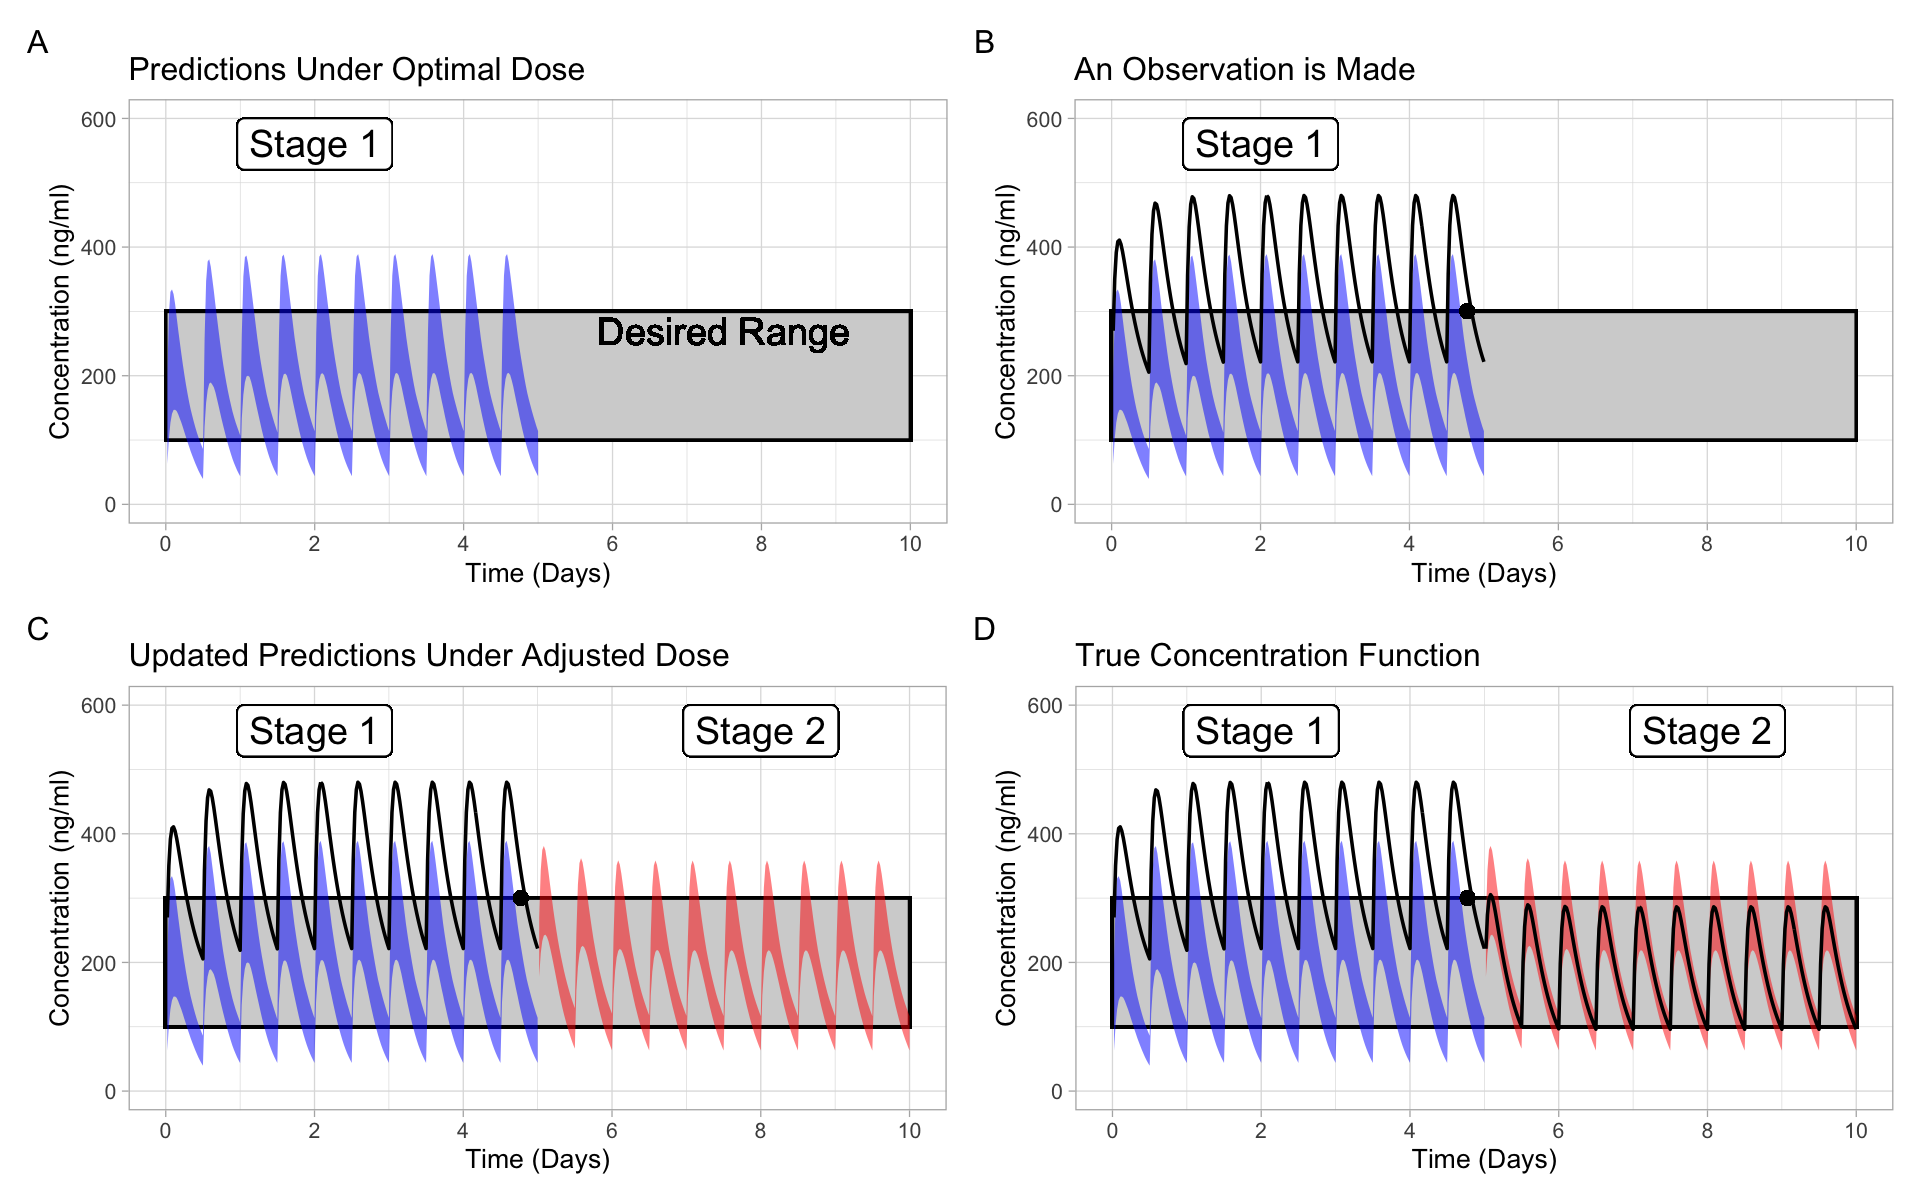
\includegraphics[width=1\linewidth]{figures/viz_of_process.png}
	\caption{
	Visual representation of the steps in our framework.	\textbf{A}  Using only clinical information, the model is used to select a dose that is expected to keep the patient in the desired range for as long as possible. The blue ribbon indicates 90\% credible interval for the latent concentration.  \textbf{B} Some time later, the patient's blood serum concentration is measured (black dot). \textbf{C}  The observation is incorporated into the model and a new dose is selected to keep the patient in range for as long as possible. The red ribbon indicates 90\% credible interval for the latent concentration after adjusting the dose. \textbf{D} The black line indicates the true latent concentration under each dose.  Note the observation (black dot) is not on the black line (true concentration) because there is measurement error, which the model accounts for.
	%Black exes indicate a discretization use to compute the reward function in each stage.
    % ^^^ I don't see these any more - maybe they are no longer used?
}
	\label{fig:processfiguresingle}
\end{figure}


		\section{Case Study}\label{ss:casestudy}

We present a case study of applying our framework to investigate the potential benefits of static and dynamic personalization of apixaban dosing. Apixaban is a direct acting anticoagulant medication used to treat active blood clots occurring with deep venous thrombosis or pulmonary embolism, or to prevent stroke in patients with atrial fibrillation. Prescribing an apixaban dose that achieves blood concentrations within an optimal range is expected to provide optimal treatment benefits while minimizing harms (e.g., serious bleeding). Clinical variables measuring age, weight, and kidney function are routinely used for dosing, and female sex, co-medications and genetic factors are known to contribute to higher circulating apixaban concentrations \cite{gulilat2020drug}. However, these variables only explain 35\% of the pharmacokinetic variability in apixaban, which serves as rationale for considering dynamic dose optimization supported by post-initiation blood concentration monitoring. 

\subsection{Bayesian Modelling}

To create the necessary model for apixaban personalization, we extend a previously proposed one-compartment Bayesian pharmacokinetic model \cite{pananos2020comparisons} to include fixed effects of covariates on pharmacokinetic parameters in order to incorporate baseline clinical information (age, sex, weight, and creatinine.)  Full details of the model structure, fitting, and diagnostic checks are provided in Appendix~\ref{ap:appendix}. We fit the model to previously-collected data on apixaban concentration \cite{tirona2018apixaban} and then use the fitted model to simulate patients with known "ground truth" pharmacokinetic parameters as described previously. We then use this population of simulated patients in our experiments to explore different modes of dose personalization and their relative benefits.

\subsection{Modes of Personalization}

%\textcolor{red}{Make these descriptions "line up" with modes in Section 3? Break out into "static" and "dynamic"?}
%\begin{enumerate}[1)]
%\item Dose selection using a hierarchical Bayesian model which does not incorporate patient covariates.  This model was presented in Pananos \& Lizotte \cite{pananos2020comparisons}.  We refer to this mode as the “No Covariate Model”.
%\item 1) and conditioning the model on a single sample from the patient taken sometime in the final 12 hours before the half way point.  At the start of the fifth day, a new dose is selected and used for the remaining time.  We refer to this mode as “No Covariate + 1 Sample”.
%\item Dose selection from M2.  A single dose is selected at the start of the regimen and is used throughout the 10 simulated days. We refer to this mode as “Covariate Model”.
%\item 3) and conditioning the model on a single sample from the patient taken sometime in the final 12 hours before the half way point.  At the start of the fifth day, a new dose is selected and used for the remaining time. We refer to this mode as “Covariate model + 1 Sample”.
%\item A two stage DTR, however the initial dose is the result of the procedure in 3).  The best time to sample the patient is then determined via Q learning. We refer to this mode as “Optimal Sampling Time”.
%\item A two stage DTR estimated via Q learning.  We refer to this mode as “Q Learning”.
%\end{enumerate}

We consider the 6 modes of personalization as outlined in \cref{ss:framework}.  To evaluate these modes of personalization, we generate 1000 simulated patients taking a dose of apixaban once every 12 hours with perfect adherence for a total of 10 days. The goal is to maximize the time spent with blood concentration level between between 100 ng/ml and 300 ng/ml. We choose this range as it is not so narrow that even optimal doses perform poorly, but not so wide that any dose can achieve high reward. For static modes of personalization, the selected initial dose is fixed over the 10 day period. For dynamic modes of personalization, some time in the second 12 hour period on the fourth day (between 108 and 120 hours after the initial dose), the simulated patient's blood concentration is measured, and then at the start of the fifth day, the dose is adjusted based on all the pre-dose clinical measurements plus the observed concentration by incorporating the new information into the Bayesian model. 

\subsubsection{Defining the Dynamic Treatment Regimes}

To implement the two dynamic modes of personalization, we estimate DTRs with two stages (the first five days, and the latter five days).  For the dynamic personalization policies our experiments, we develop a DTR for selecting the best dose for keeping a patient’s blood plasma concentration within a desired range.  In terms of the DTR, the system is the patient for whom a dose is selected, the actions correspond to selection of dose sizes (and a time in the future to sample the patient, should the DTR require that), and the reward is the proportion of time spent within the desired concentration range. The trajectories we will use to estimate the optimal Q functions are of the form

\begin{equation}\label{key}
O_1, A_1, Y_1, O_2, A_2, Y_2
\end{equation}

\noindent The interpretation of a given trajectory is:
\begin{itemize}
	\item $ O_1 $ is any pre-dose clinical measurements of the patient.  In our experiments, we consider age in years, renal function (as measured by serum creatinine in mMol/L), weight in kilograms, and dichotomous biological sex (dummy coded so that male=1 and female=0).  We choose these variables as they are known to affect the pharmacokinetics of apixaban \cite{byon2019apixaban}.  
	\item $ A_1 $ is the initial dose to provide the patient.  If the DTR allows us to specify a time in the future at which to measure the patient’s blood serum concentration, then $A_1$ is the dual action of initial dose plus a time in the future at which to measure.
	\item $ Y_1 $ is the proportion of time spent within the concentration range in the first five days.
	\item $ O_2 $ is the pre clinical measurements of the patient plus the observed concentration made on the fourth day.
	\item $ A_2 $ is the dose adjustment
	\item $ Y_2 $ is the proportion of time spent within the concentration range in the final five days after the dose adjustment.
\end{itemize}

The actions $A_j$ affect the reward $Y_j$ mediated by their effects on concentration.  For example, a larger dose will elicit larger concentrations which may put the patient in range for longer (more reward) or take them out of range for some time (less reward).  Thus, our reward function can be thought of as a composition of the reward function and the concentration function.  In our experiments, we create a mesh of $2K$ times at which we can evaluate the latent concentration and compute the reward function.  Each stage in our DTR consists of $K=240$ times (equivalent to evaluating the latent concentration function every 30 minutes after ingestion).  Let $ c_i \>,  i=1...2K \>, $ be the $ i^{th}$ latent concentration value at time $ t_i $.  The reward function in the first stage is

\begin{equation}
Y_1(H_1, A_1) = Y_1(c_1(A_1), \dots, c_K(A_1)) = \dfrac{1}{K}\sum_{i=1}^K \mathbb{I}(0.1 < c_i(A_1) < 0.3)
\end{equation}

\noindent Here, $ \mathbb{I} $ is an indicator function returning 1 if $c_i$ is between 100 ng/ml and 300 ng/ml and 0 else.
%To leverage off-the-shelf optimization tools, we approximate this reward function with a continuously differentiable function, namely
%\begin{equation}
%Y(c_1, c_2, \cdots,  c_k) = \dfrac{1}{k}\sum_{j=1}^K \exp\left( - \left[ \dfrac{c_j-0.15}{0.05} \right]^{2\beta} \right)
%\end{equation}
%
%\noindent Here, $ \beta $is a positive integer.  For sufficiently large beta, our approximation becomes arbitrarily close to our intended reward function.  In practice we set beta=5 to balance between good approximation of our intended reward and vanishing gradients impeding our optimization. 
%We suppress the dependence on the history in the definition of the reward as the reliance on the history is implicit.  The reward depends on the latent concentrations which depend on previous doses (actions) and potentially on the previous dose measurements (observations of the system).  We approximate this reward function with a continuously differentiable function to facilitate optimization.  See the appendix for details.  
\noindent The reward function in the second stage is

\begin{equation}
Y_2(H_2, A_2) = Y_1(c_{K+1}(A_2), \dots, c_{2K}(A_2)) = \dfrac{1}{K}\sum_{i=1}^K \mathbb{I}(0.1 < c_{K+i}(A_2) < 0.3)
\end{equation}

Our stage 2 optimal Q function is then

\begin{equation}
Q_{2}^{\mathsf{opt}}\left(H_{2}, A_{2}\right)=E\left[Y_2\left(c_{K+1}(A_2), \cdots, c_{2K}(A_2)\right) \Bigg\vert H_{2}, A_{2}\right] \>,
\end{equation}

\noindent and our stage 1 optimal Q function is

\begin{equation}
Q_{1}^{\mathsf{opt}}\left(H_{1}, A_{1}\right)= E \left[Y_1\left(c_{1}(A_1),  \cdots, c_{K}(A_1)\right)+\max _{a_{2}} Q_{2}^{\mathsf{opt}}\left(H_{2}, a_{2}\right) \Bigg\vert H_{1}, A_{1}\right]
\end{equation}

We seek to maximize the stage 1 optimal Q function to learn the optimal DTR for dosing patients under the constraint we can measure them at most once and are limited to the aforementioned pre-dose clinical variables.  The interpretation of stage 1 optimal Q function is as follows:\textit{ Given the pre-dose clinical variables of the patient and a proposed initial dose and measurement time, the stage 1 optimal Q function gives the expected proportion of time the patient’s blood serum concentration is between 100 ng/ml and 300 ng/ml assuming that we provide the patient with the best dose possible at the start of the $ 5^{th} $ day.}  The decision rules which choose $ A_1 $ and $ A_2 $ to maximize these functions constitutes the estimated optimal DTR.

%
%The concentration values $ c_j $ in the optimal Q functions are latent, meaning we have no direct access to them in practice. Furthermore, obtaining measurements with high enough frequency so that the reward is faithfully estimated would be too burdensome on the patient. 

\subsection{Evaluating Modes of Personalization}

We measure the performance of different modes in terms of \textit{regret}, the difference between theoretically largest possible return if the individual's PK parameters were precisely known and the achieved return by each mode of personalization. The results are shown in \cref{fig:modelsofpersonalizationdifferences}, ordered from least amount of information and burden (top) to most amount of information and burden (bottom) and colored by their personalization strategy (static or dynamic).

Modes of personalization which use less information have larger regret.  The One Size Fits All approach (which uses no information about the patient) performs worst with a median regret of 0.145.  The distribution of regrets for this mode is right skewed with some exceeding 0.95, meaning the patient could have been in range for nearly the entire time if the correct PK parameters were known, but the mode selected a dose which failed to put the patient in range. 

The Clinical Variables mode nearly cuts the regret in half, achieving a median regret of 0.086 with smaller right skew.  Modes which use observed concentration information (Clinical Variables + One Sample, Optimal Sampling Time, and Optimal Sequential Dosing) lead to slightly lower median regrets  (0.075, 0.076, 0.079 respectively) as compared to the Clinical Variables mode.

\begin{figure}
	\centering
	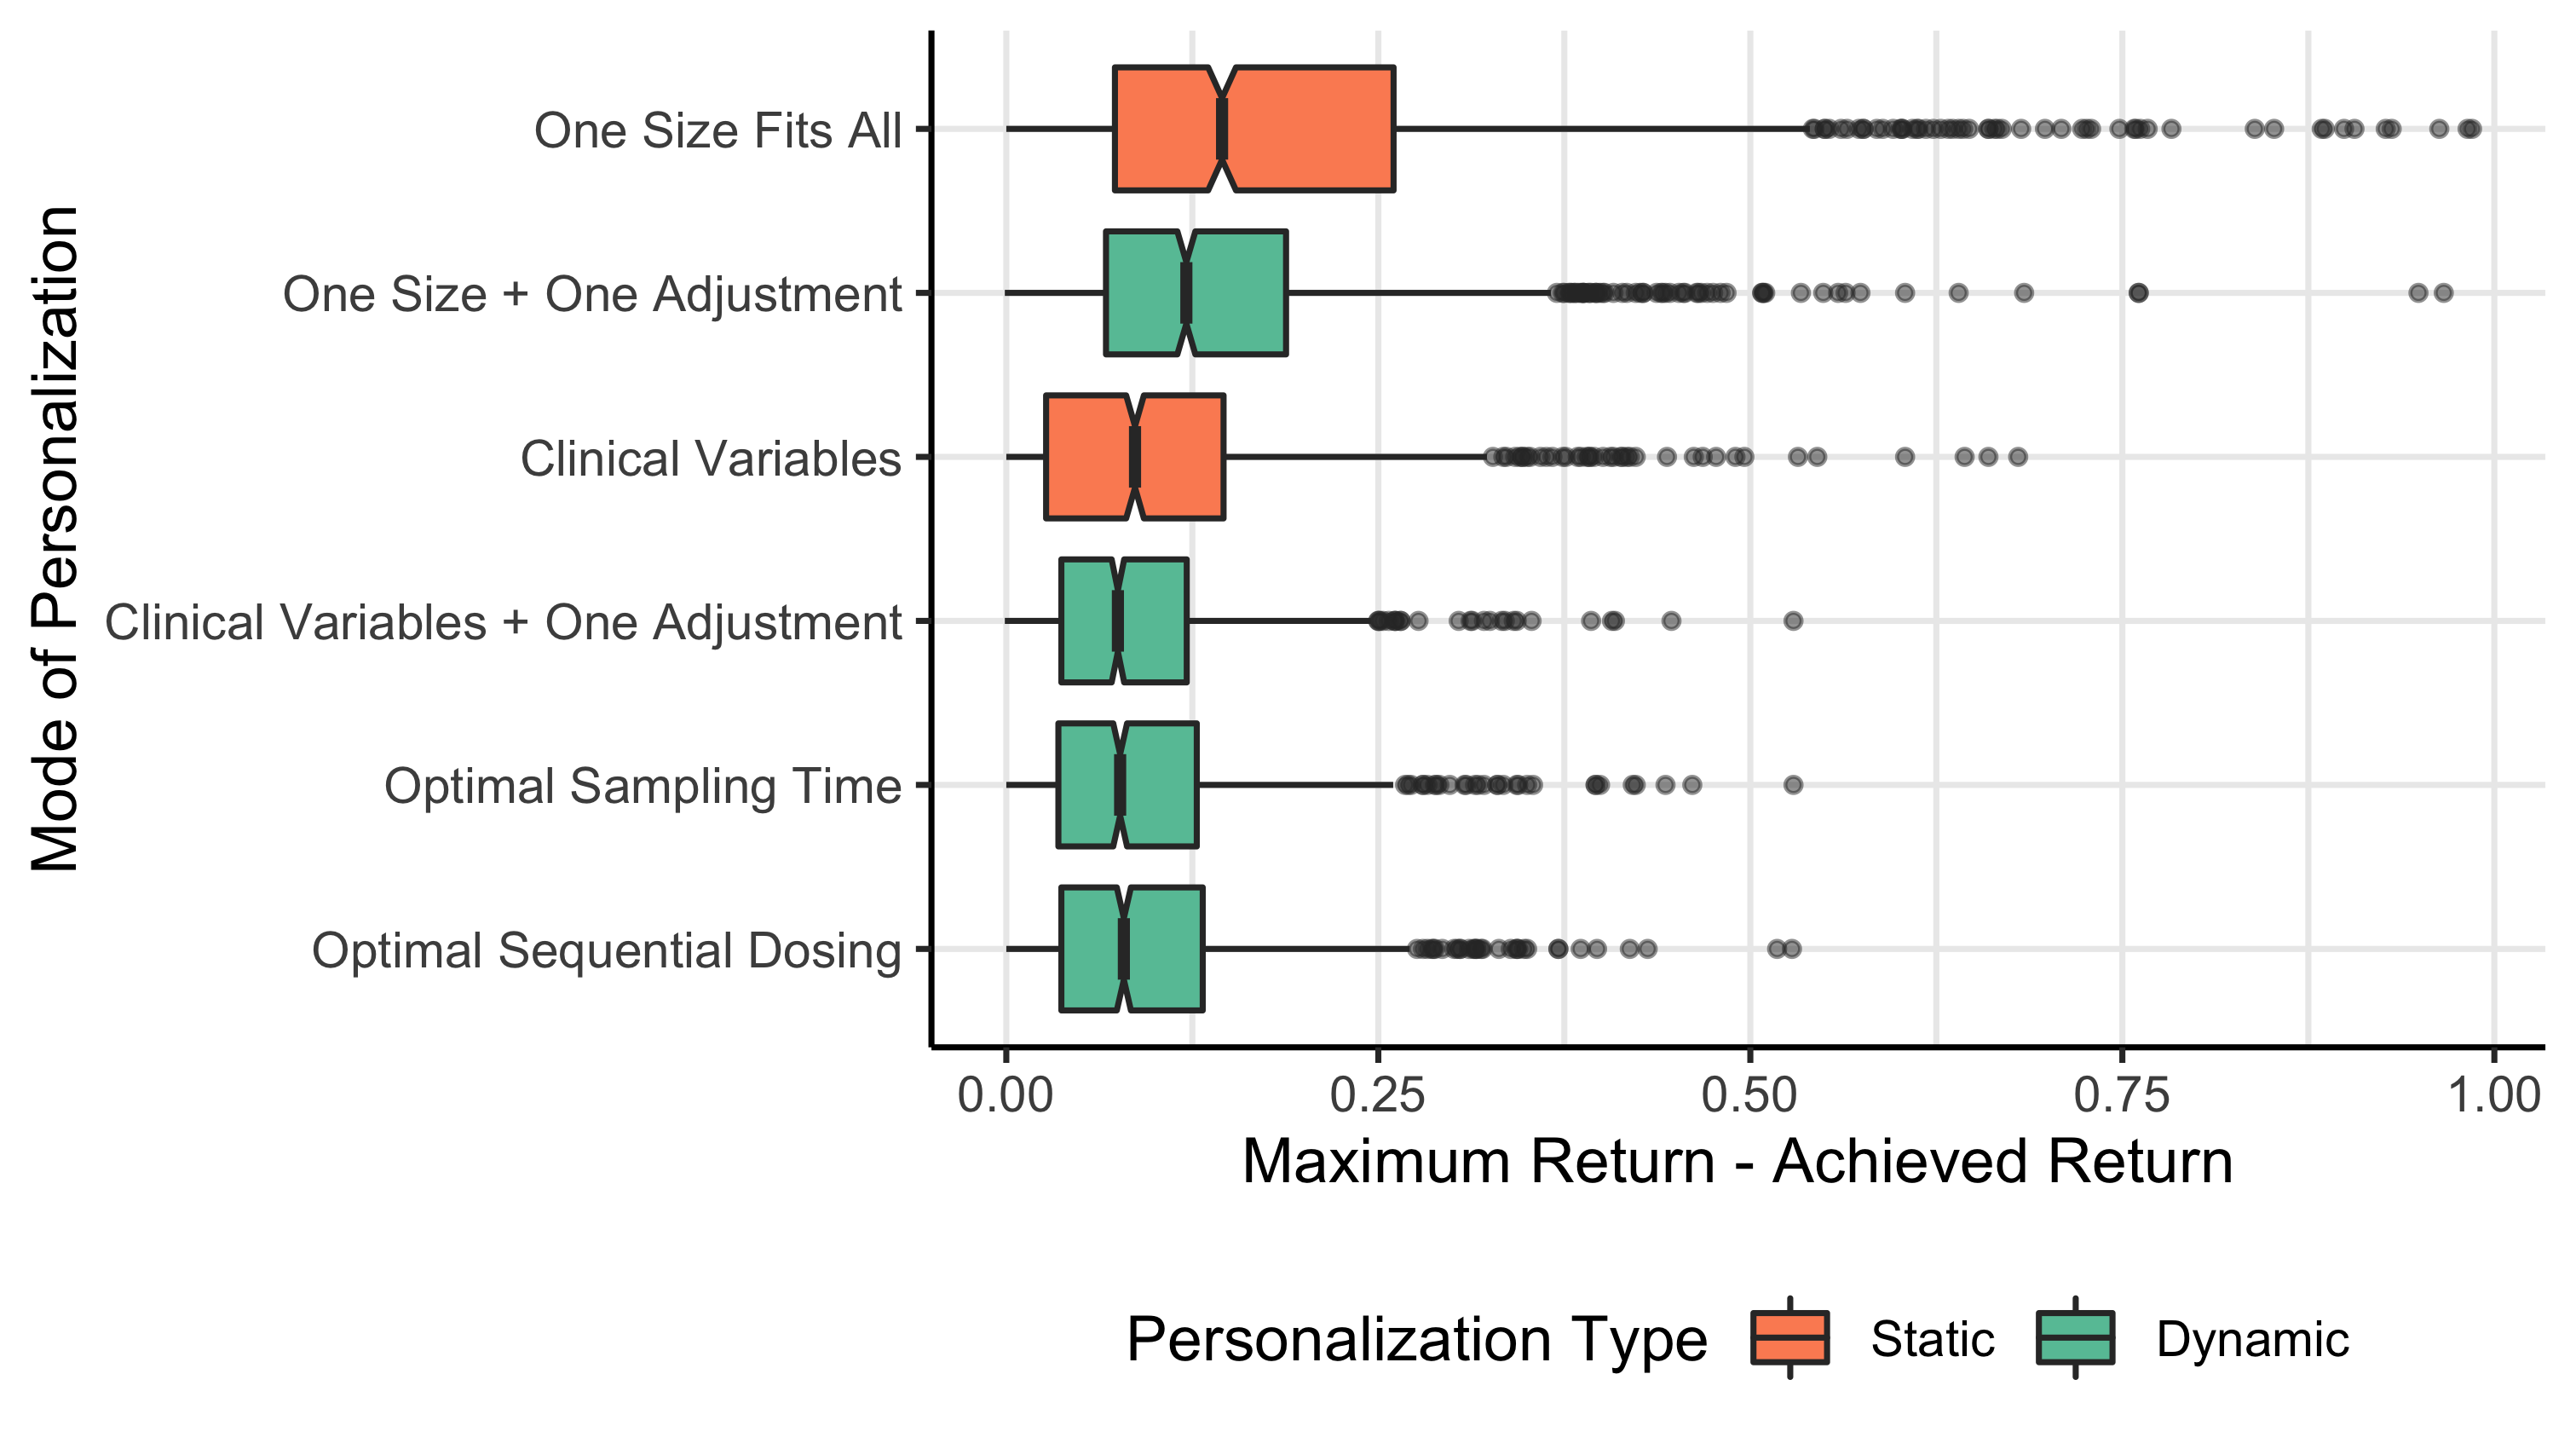
\includegraphics[width=1\linewidth]{figures/models_of_personalization_differences}
	\caption{Boxplots of the \textit{regret} -- the difference between the largest possible return and the achieved return for each of the 1000 simulated patients. patients who achieve a return close to their maximum possible return have a regret near 0, while patients who achieve a return less than their maximum possible have larger regrets, with the largest possible regret being 1.}
	\label{fig:modelsofpersonalizationdifferences}
\end{figure}

		\section{Limitations}

%We have examined six modes for making decisions.  The next mode improves on a deficiency of the previous mode in a natural manner, and so our experiment constitutes a kind of ablation study.  We believe the decision making aspect of our study extracts information in a responsible way and uses the best decision making methodology available.  That being said, the experiment is not without limitations.

%The Bayesian model of the pharmacokinetics is integral to the methodology we present.  Any shortcomings in the model affect the quality of the decision and decision process.  Bayesian models are not as ubiquitous as other models in pharmacology, and so particular expertise is required for model development and evaluation.  That expertise increases the implementation burden of any decision process involving Bayesian models.  However, we demonstrate how one such model can be constructed in a past study \cite{pananos2020comparisons} and include open sourced code and data for practitioners to replicate our model fitting.

Our framework relies on the quality of the Bayesian model used to predict plasma concentrations. The data required to construct a high quality Bayesian model of pharmacokinetics require multiple observations of a single patient over an extended time, preferably over multiple well timed doses with near perfect adherence.  Obtaining such data requires well organized efforts and is high burden for both investigators and participating subjects.  This makes acquiring a robust Bayesian model for use in dose personalization difficult. For this reason, our framework is not intended to replace prospective evaluation of personalized medicine programs; rather it is intended to estimate relative performance given existing evidence so that the most promising modes of personalization can be identified for potential implementation and further study.


\subsection{Related Work}

\textbf{Individualized Dose Rules} Much recent work on individualized dose rules (also sometimes called personalized dosing rules, or personalized treatment rules, or personalized treatment decisions) focuses on estimation of the value function and use of Q-learning or similar techniques for estimation of the optimal policy. Chen et. al \cite{chen2016personalized} extended an application of O-learning from Zhao et. al \cite{zhao2012estimating} to the case with continuous treatment values (i.e. doses).  Laber and Zhao \cite{laber2015tree} proposed an approach to estimating optimal personalized treatment rules using decision trees, placing emphasis on their interpretability. Li et.al \cite{li2020utility} estimate individualized dose rules by directly balancing risks of efficacy and outcomes using a large number of biomarkers and patient covariates and an $\ell_1$ penalty. Park et. al \cite{park2021single} demonstrate a semi-parametric approach to estimating the dose by covariate interaction effects on treatment response and demonstrate this approach on Warfarin dose outcomes with clinical and pharmacogenetic data.  Rich et. al \cite{rich2014simulating} design a sequential multiple assignment randomized trial for optimal dose selection, and demonstrate their design by simulating data from a pharmacokinetic model based on Warfarin. They contrast Q-learning and G-estimation for estimating the parameters of various value functions which incorporate various different sources of information into the individualization process.

In many of these studies, the value function must be estimated, often with a suitably flexible regression method.  Because the value function must be estimated, there is a risk of model misspecification.  In our work, we need not estimate the value function because it is a function of latent concentrations.  We integrate our uncertainty over these latent concentrations and pass them to our value function directly.  This avoids possible misspecification of the value function, allowing investigators to focus their modelling on the pharmacokinetics.


\section{Conclusions}\label{ss:discussion}

%Including age, sex, weight, and creatinine in our Bayesian model improved the inferences from that model.  Though the predicted concentrations and estimates of uncertainty changed negligibly, the covariates explained residual confounding in the random effects. This results in a model which better explains the observed variation in the data and hence should generate more plausible data for simulation.

%In the following, we discuss the results of our case study and some broader potential implications for personalized medicine policy.

%Working subsection titles - not sure if they stay
%\subsection{Comparing Modes of Personalization}

As expected, modes of personalization that use more information result in lower regret (larger achieved rewards.)  The static Clinical Variables mode balances relatively low implementation burden with high reward. However, there is right skew in the distribution of regret, with some `outliers' who are at risk of obtaining less than half of their best possible return. If avoiding this risk is important, the Clinical Variables + One Adjustment mode may be preferable, even though it imposes additional burden.

The Optimal Sampling Time and Optimal Sequential Dosing modes use the same information as Clinical Variables + One Adjustment, but impose more burden on the patient and clinic. Both require samples be taken at specified times, and the second uses a more complex optimization procedure. Neither of these improved performance beyond the simpler modes in our study. There are two characteristics of our study that may explain this result. First, the clinical variables used are known to affect the pharmacokinetics of apixiban and are useful for predicting concentrations for static personalization, hence their use alone makes it possible to choose good doses. In other settings where clinical variables are not as predictive, we would expect dynamic personalization to have a bigger advantage. Second, the elimination rates $k_e$ in our study were relatively high. This means that the effect of an initial dose on levels at the time subsequent doses are taken (i.e., a day later) is relatively small, so that doses can be optimized largely independently. If this were not the case, optimization using Q-learning would be expected to be more important to ensure that initial doses were not too large to successfully adapt later.

% \subsection{Future Work}

% Because the data required to build reliable Bayesian pharmacokinetic models are difficult to collect in practice, research into developing these models from observational data may prove fruitful in extending this work. If clinics record data on measured blood concentrations, they may have dozens or hundreds of subjects with only one or two measurements per subject.  Moreover, the subjects in question may be on multiple drugs or have comorbidities which may affect the pharmacokinetics of the drug under study.  Additional research into constructing Bayesian models which can adjust for polypharmacy and comorbidities while learning an individual’s pharmacokinetics from a large but sparse sample would drive this work towards being easier to implement in practice.


% It is clear that there are tradeoffs between achieving a reward close to what is theoretically largest and taking on additional clinic and implementation burden, and that tradeoff should be examined on a case-by-case basis.  Context is crucial, and how we adapt to that context is perhaps a question in need of closer examination.  Traditional methods of personalization include conditioning only on a subject’s covariates (not unlike the Clinical Variables mode we present here).  But of course patients are not their age, sex, weight, and creatinine.  Additionally, safety information and best available practices might change in the future as more research on drugs is performed. Were new safety information to be published, the reward function may need to be re-designed, which may result in a new mode of personalization being more/less preferable or more/less feasible.  Any number of factors in flux can change the context in which personalization occurs, and that change in context may prompt for a re-evaluation in how personalization is done.

%We do not offer recommendations on how personalization for apixaban should be done because this depends on the context of the health system and population where such personalization would be deployed. Rather, we offer a framework for developing strategies of personalization and evaluating their performance against their implementation and patient and provider burden.  Analyses can be adapted where needed, either through the reward function, or by adjusting when the clinic is able to take measurements, or by including additional information such as genotype in the Bayesian model. Each of these can also be done within established systems when new evidence or data become available. Using this framework, clinics have flexibility to tailor their personalization to the populations they serve.

%Working subsection titles - not sure if they stay
%\subsection{Relating Results to Policy Decisions}



%An additional expertise burden is added as machine learning (used interchangeably with the term “artificial intelligence”) is adopted into personalized medicine initiatives.  Cutting edge machine learning models for prediction or decision making can be prohibitively burdensome to implement effectively. Failure to carefully implement a prediction model may result in pernicious bias inadvertently affecting subpopulations, as was found to be the case in algorithms for credit scoring \cite{barocas2016big}, crime prediction \cite{lum2016predict}, and hiring \cite{ajunwa2020paradox}.  A 2019 study found an instance of this bias in a widely used risk scoring algorithm in healthcare \cite{obermeyer2019dissecting}, demonstrating that despite the best intentions of those involved, the use of a model can lead to worse rather than better care if investigators are not careful in considering what sorts of bias may be present in the data used to train these models.  Implementation of new approaches and methods requires the close collaboration of experts in data science  with physicians, domain experts, and other stakeholders.  Close collaboration should allow for domain experts to identify what kinds of biases the data might have, and for data science experts to implement methods to help ameliorate that bias (or to admit the data are not fit for purpose).  The result of iterating on this collaborative process (wherein domain experts help inform the approaches methodologists take, and the methodologists provide model checks which help domain experts decide if decisions from the model are reasonable or suspicious) is a model which more closely aligns with domain expertise, a model which is sufficiently flexible to capture the true data generating mechanism, an effective use of data, a more transparent modelling process, and calibrated expectations surrounding algorithms and their abilities \cite{frohlich2018hype}.  Presently, this form of collaboration between methodologists and domain experts is not the norm, with development of machine learning solutions in healthcare being developed in silos \cite{wiens2019no}.  These burdens may be surmountable for some, but the question then turns to if the result is worth the expense.   Answering that question is difficult without an idea how the additional burden of collecting data, or implementing new algorithms, will benefit the clinic or the patient subject to inherent constraints. 




\section{Implications}

Any decision to implement personalized medicine must assess the costs and benefits of doing so. Despite the potential for personalized medicine to reduce health care costs \cite{looff2016economic,shabaruddin2015economic}, the cost of patient testing and monitoring, personnel, and training required to operate a personalized medicine clinic carry a burden, and it is not yet clear in what circumstances personalized medicine is cost effective.  In their 2019 scoping review of personalized medicine cost effectiveness, Kasztura et al \cite{kasztura2019cost} found that willingness-to-pay thresholds vary wildly from country to country (citing that cost per quality adjusted life year (QALY) for some modes of personalized medicine range from \$20,000 USD per QALY in Europe and the United Kingdom to \$200,000 USD per QALY in the United States).  This high variability means the burden required for start up may result in a positive return on investment in some areas but not others. This variability should prompt would be adopters to more closely examine whether taking on the initial burden is worth the result.

Others have noted that  much work on personalized medicine has not centred the needs, constraints, and utilities of the patient \cite{rogowski2015concepts, di2017personalized}. Patients can be burdened by frequent followup for clinical measurement (as in the case with warfarin), be burdened by costly expenses related to obtaining care, or may be more risk adverse/tolerant than the ``typical'' patient. As an example, transportation has been found to be a large financial burden for patients receiving cancer treatment \cite{houts1984nonmedical}, and continues to burden patients, with a 2020 study finding that the cost of parking alone can climb as high as \$1600 over the course of treatment in the United States \cite{lee2020assessment}.  Additional visits to a clinic have the potential to further burden patients by requiring them to miss a day of work, and find means of childcare during their absence (if necessary). Incorporating patient preferences and reducing the burden of personalization on the patient can result in sustained adherence \cite{elliott2008understanding}, thereby increasing effectiveness and further preventing adverse events.

The complexity of balancing these burdens means that Implementation decisions made at the organizational level need to attend to a broad array of evidence and contextual factors. Know4Go \cite{martin2016hospital} is one framework for explicitly considering factors from expanded domains of influence surrounding adoption of new technologies/interventions in a healthcare setting (like a clinic or hospital). These expanded domains of influence include: social, legal, ethical, environmental/institutional, political, entrepreneurial/innovative, research opportunity, and reversibility factors in conjunction with objective evidence of benefits versus risks, systematic review, and costs.  Broadly, once evidence has been synthesized through systematic review and/or meta-analysis, the evidence is contextualized to local healthcare system perspective.  Evidence is converted onto a benefit scale, derived from the number of patients likely to benefit from adoption of the technology/intervention.  Budget impact of the adoption is estimated using costing data from the hospital/clinic, and new technologies can be triaged according to their impact and cost.  

Policy decisions around personalization are complex. They carry burden for health systems and patients that vary widely by context. While there are frameworks like Know4Go for navigating these decisions, applying them requires quality evidence for the potential benefits of different kinds of personalization, even for deciding on potential pilot studies. Our framework can produce evidence for the potential effectiveness of a range of modes of personalization to inform organization-level decisions surrounding the investigation and implementation of personalized medicine programs that reduce cost, respect burden, and improve outcomes.



		\section{Appendix}\label{ap:appendix}

\subsubsection{Bayesian PK Model Details}

The Bayesian model used to predict personalized concentration in response to dose, which we refer to as $ \mathcal{M}_1 $, is 

\begin{align}\label{model_M1}
	y_{i,j} &\sim \Lognormal  \left(  C_i(t_j)  , \sigma^2_y \right)  \\
	\sigma^2 &\sim \Lognormal \left( 0.1, 0.2 \right)\\	
	C_i(t_j) &= \begin{dcases}
	\frac{D_{i} \cdot F}{C l_{i}} \cdot \frac{k_{e, i} \cdot k_{a, i}}{k_{e, i}-k_{a, i}}\left(e^{-k_{a, i}\left(t_{j}-\delta_{i}\right)}-e^{-k_{e, i}\left(t_{j}-\delta_{i}\right)}\right) & t_j>\delta_i \\
	0 & \mbox{else}
	\end{dcases}\\
	k_{e,i} &= \alpha_i \cdot k_{a,i}\\
	k_{a,i} &= \dfrac{\log(\alpha_i)}{t_{max, i}\cdot(\alpha_i-1)}\\
	\delta_i &\sim \operatorname{Beta}(\phi, \kappa) \\
	\operatorname{logit}(\alpha_i) \vert \beta_\alpha, \sigma^2_\alpha &\sim \Normal(\mu_\alpha + \mathbf{x}_i^T \beta_\alpha, \sigma^2_\alpha)\\
	\log(t_{max, i}) \vert \beta_{t_{max}}, \sigma_{t_{max}} &\sim \Normal(\mu_{t_{max}} + \mathbf{x}^T_i \beta_{t_{max}}, \sigma^2_{t_{max}}) \\
	\log(Cl_i) \vert \beta_{Cl}, \sigma_{Cl} &\sim \Normal(\mu_{Cl} + \mathbf{x}^T_i \beta_{Cl}, \sigma^2_{Cl}) \\ \nonumber \\
	p(\phi) &\sim \operatorname{Beta}(20, 20)\\
	p(\kappa) &\sim \operatorname{Beta}(20, 20)\\
	p(\mu_{Cl}) &\sim \Normal(\log(3.3), 0.15^2)\\
	p(\mu_{t_{max}}) &\sim \Normal(\log(3.3), 0.1^2)\\
	p(\mu_{\alpha}) &\sim \Normal(-0.25, 0.5^2)\\
	p(\sigma_y) &\sim \Lognormal(\log(0.1), 0.2^2)\\
	p(\sigma_{\mathit{Cl}}) &\sim \Gmma(15, 100)\\
	p(\sigma_{t_{max}}) &\sim \Gmma(5, 100)\\
	p(\sigma_{\alpha}) &\sim \Gmma(10, 100)\\
	p(\beta_{Cl, k}) &\sim \Normal(0, 0.25^2) \quad k = 1 ...	 4\\
	p(\beta_{t_{max}, k}) &\sim \Normal(0, 0.25^2) \quad k = 1 ... 4\\	
	p(\beta_{\alpha, k}) &\sim \Normal(0, 0.25^2) \quad k = 1 ... 4
\end{align}

Here, normal distributions are parameterized by their mean and variance, lognormal distributions are parameterized by the mean and variance of the random variable on the log scale, and gamma distributions are parameterized by their shape and rate.  The $\mu$ in the model above represent population means on either the log or logit scale, the $\beta$ are regression coefficients for the indicated pharmacokinetic parameter, the sigmas are the population level standard deviations on the log or logit scale, $\delta$ is aparameter which relaxes the assumption that the dose is absorbed into the blood immeditately upon ingestion, $F$ is the bioavailability of apixiban (which we fix to 0.5 \cite{byon2019apixaban}) and $D$ is the size of the dose in milligrams.  All continuous variables were standardized using the sample mean and standard deviation prior to being passed to the model. 

\begin{table}\label{tab:coefs}
	\centering
	\begin{tabular}[t]{rccc}
		\toprule
		& $\beta_\alpha$ & $\beta_{\mathit{Cl}}$ & $\beta_{t_{max}}$\\
		\midrule
		\cellcolor{gray!6}{Age} & \cellcolor{gray!6}{-0.08 (-0.27,0.1)} & \cellcolor{gray!6}{0.01 (-0.06,0.08)} & \cellcolor{gray!6}{-0.01 (-0.1,0.08)}\\
		Creatinine & -0.06 (-0.25,0.14) & 0.02 (-0.05,0.09) & -0.05 (-0.14,0.04)\\
		\cellcolor{gray!6}{Sex} & \cellcolor{gray!6}{-0.2 (-0.53,0.15)} & \cellcolor{gray!6}{0.39 (0.23,0.54)} & \cellcolor{gray!6}{-0.01 (-0.18,0.15)}\\
		Weight & 0.32 (0.11,0.55) & 0.2 (0.12,0.27) & 0.09 (0.01,0.18)\\
		\bottomrule
	\end{tabular}
	\caption{Posterior means for coefficients for each covariate in our pharmacokinetic model.  In parantheses are 95\% credible interval estimates.}
\end{table}
Once fit, $ \mathcal{M}_1$ can be used to predict the pharmacokinetics of new patients, using the patient’s covariates as predictors.  To do so, the marginal posterior distributions for $ \mu_{\mathit{Cl}} $, $ \mu_{t_{max}} $, $ \mu_{\alpha}$, $ \beta_{\mathit{Cl}} $, $ \beta_{t_{max}} $, $ \beta_{\alpha} $, $ \sigma_{\mathit{Cl}} $, $ \sigma_{t_{max}} $, $ \sigma_{\alpha} $, and $ \sigma_y $ must be summarized.  We use maximum likelihood on the posterior samples to summarize the marginal posterior distributions. We model the population means  and regression coefficients as normal, and the standard deviations  as gamma.  The maximum likelihood estimates are used to construct priors for a new model, which we call $ \mathcal{M}_2 $. We construct $ \mathcal{M}_2 $ so as to be able to predict plasma concentration after multiple doses (of potentially different sizes) administered over time, and remove the time delay ($ \delta $) to simplify our simulations.  Model priors for $ \mathcal{M}_2 $ are then 

\begin{align}
	p(\mu_{\mathit{Cl}}) & \sim \Normal(0.5, 0.04) \\
	p(\mu_{t_{max}}) & \sim \Normal(0.93, 0.05) \\
	p(\mu_\alpha) &\sim \Normal(-1.35, 0.13)\\
									\nonumber \\
	p(\sigma_{\mathit{Cl}}) &\sim \Gmma(69.15, 338.31)\\
	p(\sigma_{t_{max}}) &\sim \Gmma(74.96, 349.56)\\
	p(\sigma_{\alpha}) &\sim \Gmma(10.1, 102.07)\\
									\nonumber\\
	p(\beta_{\mathit{Cl}, 1}) &\sim \Normal(0.39, 0.08^2)\\
	p(\beta_{\mathit{Cl}, 2}) &\sim \Normal(0.19,0.04^2)\\
	p(\beta_{\mathit{Cl}, 3}) &\sim \Normal(0.02,0.04^2)\\
	p(\beta_{\mathit{Cl}, 4}) &\sim \Normal(0.01,0.04^2)\\
									\nonumber\\
	p(\beta_{t_{max}, 1}) &\sim \Normal(-0.01, 0.08^2)\\
	p(\beta_{t_{max}, 2}) &\sim \Normal(0.09,0.05^2)\\
	p(\beta_{t_{max}, 3}) &\sim \Normal(-0.05,0.04^2)\\
	p(\beta_{t_{max}, 4}) &\sim \Normal(-0.01,0.04^2)\\
										\nonumber\\
	p(\beta_{\alpha, 1}) &\sim \Normal(-0.19, 0.17^2)\\
	p(\beta_{\alpha, 2}) &\sim \Normal(0.33,0.11^2)\\
	p(\beta_{\alpha, 3}) &\sim \Normal(-0.06,0.1^2)\\
	p(\beta_{\alpha, 4}) &\sim \Normal(-0.09,0.1^2)\\
\end{align}

For our experiments, we generate the pharmacokinetic parameters of 1000 simulated patients from the prior predictive model of $ \mathcal{M}_2 $. Bayesian models are generative models, meaning they can generate pseudodata by drawing random variables according to the model specification going from top (model priors) to bottom (model likelihood).  To do so, we begin by resampling 1000 tuples of age, sex, weight, and creatinine from the dataset used to fit $ \mathcal{M_1} $. We sample one draw of r $ \mu_{\mathit{Cl}} $, $ \mu_{t_{max}} $, $ \mu_{\alpha}$, $ \beta_{\mathit{Cl}} $, $ \beta_{t_{max}} $, and $ \beta_{\alpha} $  from their respective prior distributions in  $ \mathcal{M}_2 $. The values of these parameters remained fixed for all 1000 patients. Conditioned on the values of these mus and betas, we compute the expectation of the population distribution for each pharmacokinetic parameter by computing $ \mu_{\mathit{Cl}} + \mathbf{x}^T \beta_{\mathit{Cl}} $, $ \mu_{t_{\max}} + \mathbf{x}^T \beta_{t_{max}} $,  $ \mu_{\alpha} + \mathbf{x}^T \beta_{\alpha} $, where $\mathbf{x}^T$ is the resampled tuple.  From the prior distribution of M2, we sample one draw of$ \sigma_{\mathit{Cl}} $, $ \sigma_{t_{max}} $, $ \sigma_{\alpha} $, and $ \sigma_y $.  These remained fixed for all 1000 patients. Using the previously computed expectations and $\sigma$, we sample 1000 tuples of pharmacokinetic parameters, one for each of the simulated patients.  The clearance rate and time to max concentration were sampled assuming a lognormal distribution.  Alpha was sampled using a logitnormal distribution. The pharmacokinetics can then be determined conditional on the pharmacokinetic parameters. Each of simulated patients' pharmacokinetic parameters remained fixed through the experiments.  We simulate the latent concentration using $ C(t) $ as written in $\mathcal{M}_2$, and can simulate observed concentrations by drawing a sample from a lognormal distribution with mean $\ln(C(t))$ and standard deviation $ \sigma_y$

We use Stan, an open source probabilistic programming language, for fitting our Bayesian models via Hamiltonian Monte Carlo (a Markov Chain Monte Carlo technique) and computing markov chain diagnostics. Twelve chains are initialized and run for 2000 iterations each (1000 for warmup allowing the Markov chain the opportunity to find the correct target distribution and 1000 to use as samples from the posterior).


\subsubsection{Diagnostics For Bayesian Models Fit Via MCMC}

Once the form of the model is specified, creating simulated patients or estimating the PK parameters of a real patient requires computation of or sampling from the posterior distribution of the relevant variables given the relevant data. However, exact computation of the posterior distribution is intractable for all but very simple models, so Markov chain Monte Carlo (MCMC) techniques are often used to approximate the expectations with respect to the posterior distribution.  Presently, the gold standard for generating samples from the posterior is Hamiltonian Monte Carlo (HMC), which works by generating a sequence of samples that ``explores'' the posterior distribution by solving a system of ordinary differential equations which describe the motion of an imaginary particle as it rolls along the surface of the log posterior density.  Many implementations of HMC come with diagnostics which monitor the behaviour of the Markov chains that are used to generate samples and help to ensure that they are representative of the posterior distribution. That these Markov chains behave well is crucial, as any inferences about or from the model are obtained from samples generated by the chains. To assess the quality of the Markov chains, several diagnostics are commonly used including: number of divergences, the Gelman-Rubin convergence diagnostic, and effective sample size \cite{betancourt2018conceptual}.

In practice, several Markov chains are used simultaneously to generate samples from the posterior. The chains are assessed with within-chain and between-chain diagnostics. First, individual chains may sometimes \textit{diverge}. A divergence in a Markov chain indicates that the HMC Markov chain has encountered a region of high curvature in the posterior distribution which cannot be adequately explored.  Consequently, Monte Carlo estimators of any expectations can be biased due to incomplete exploration of the posterior distribution.  It is important that none of the Markov chains generated by HMC display a divergence, and that many chains (typically 4 or more) are initialized and are allowed to explore the posterior distribution. 

Having ensured that no chains are diverging, a group-level diagnostic is used to assess whether all chains have converged to the same limiting distribution.  The \textit{Gelman-Rubin (sometimes called $\hat{R}$) convergence diagnostic} is designed to detect if the Markov chains have converged to the same distribution by measuring the within-chain variance to the between chain-variance. In practice, $1.05<\hat{R}$ indicates that there is poor mixing of the Markov chains and inference from the samples should not be performed lest the Monte Carlo estimators are biased by this poor mixing.

Even if the chains do not exhibit divergences and arrive at the same limiting distribution, the Markov chains could still exhibit high within-chain correlation, thereby increasing the uncertainty of estimation of key posterior quantities such as means, variances, or quantiles \cite{brooks2011handbook}.  The \textit{effective sample size} is a measure of how much the within chain autocorrelation increases uncertainty estimates.  Presently, the guidance is that the effective sample size ratio should be larger than $100 \times (\mbox{number of chains})$ \cite{vehtari2019rank}.

In addition to monitoring divergences, Gelman-Rubin convergence diagnostics, and effective sample sizes, the model should be evaluated against existing domain knowledge.  Evaluating that the model has learned appropriate  behaviour (e.g. that as one quantity increases, another should decrease) can be performed by plotting model predictions.  Additionally, \textit{posterior predictive checks} -- generating synthetic data  from the model's posterior distribution and comparing against the real data -- can be performed to ensure the model is not generating data which are physically impossible or completely unrealistic. Once the model is fit, important diagnostics indicate no pathological behaviour, and the model is deemed to fit the data sufficiently well, the model can then used to generate synthetic pharmacokinetic data for use in experiments to compare different forms of personalization. Each generated data point may be thought of as one synthetic patient, with observed covariates and observed pharmacokinetic parameters. These parameters, which are never observed in real data, allow us to compute the effects of any dosing decisions (which are made \textit{without} direct knowledge of the parameters), and thus allow us to evaluate the performance of different modes of personalized dosing on the sampled population. 

\subsubsection{Bayesian Model Diagnostics for Case Study}

\begin{figure}
	\centering
	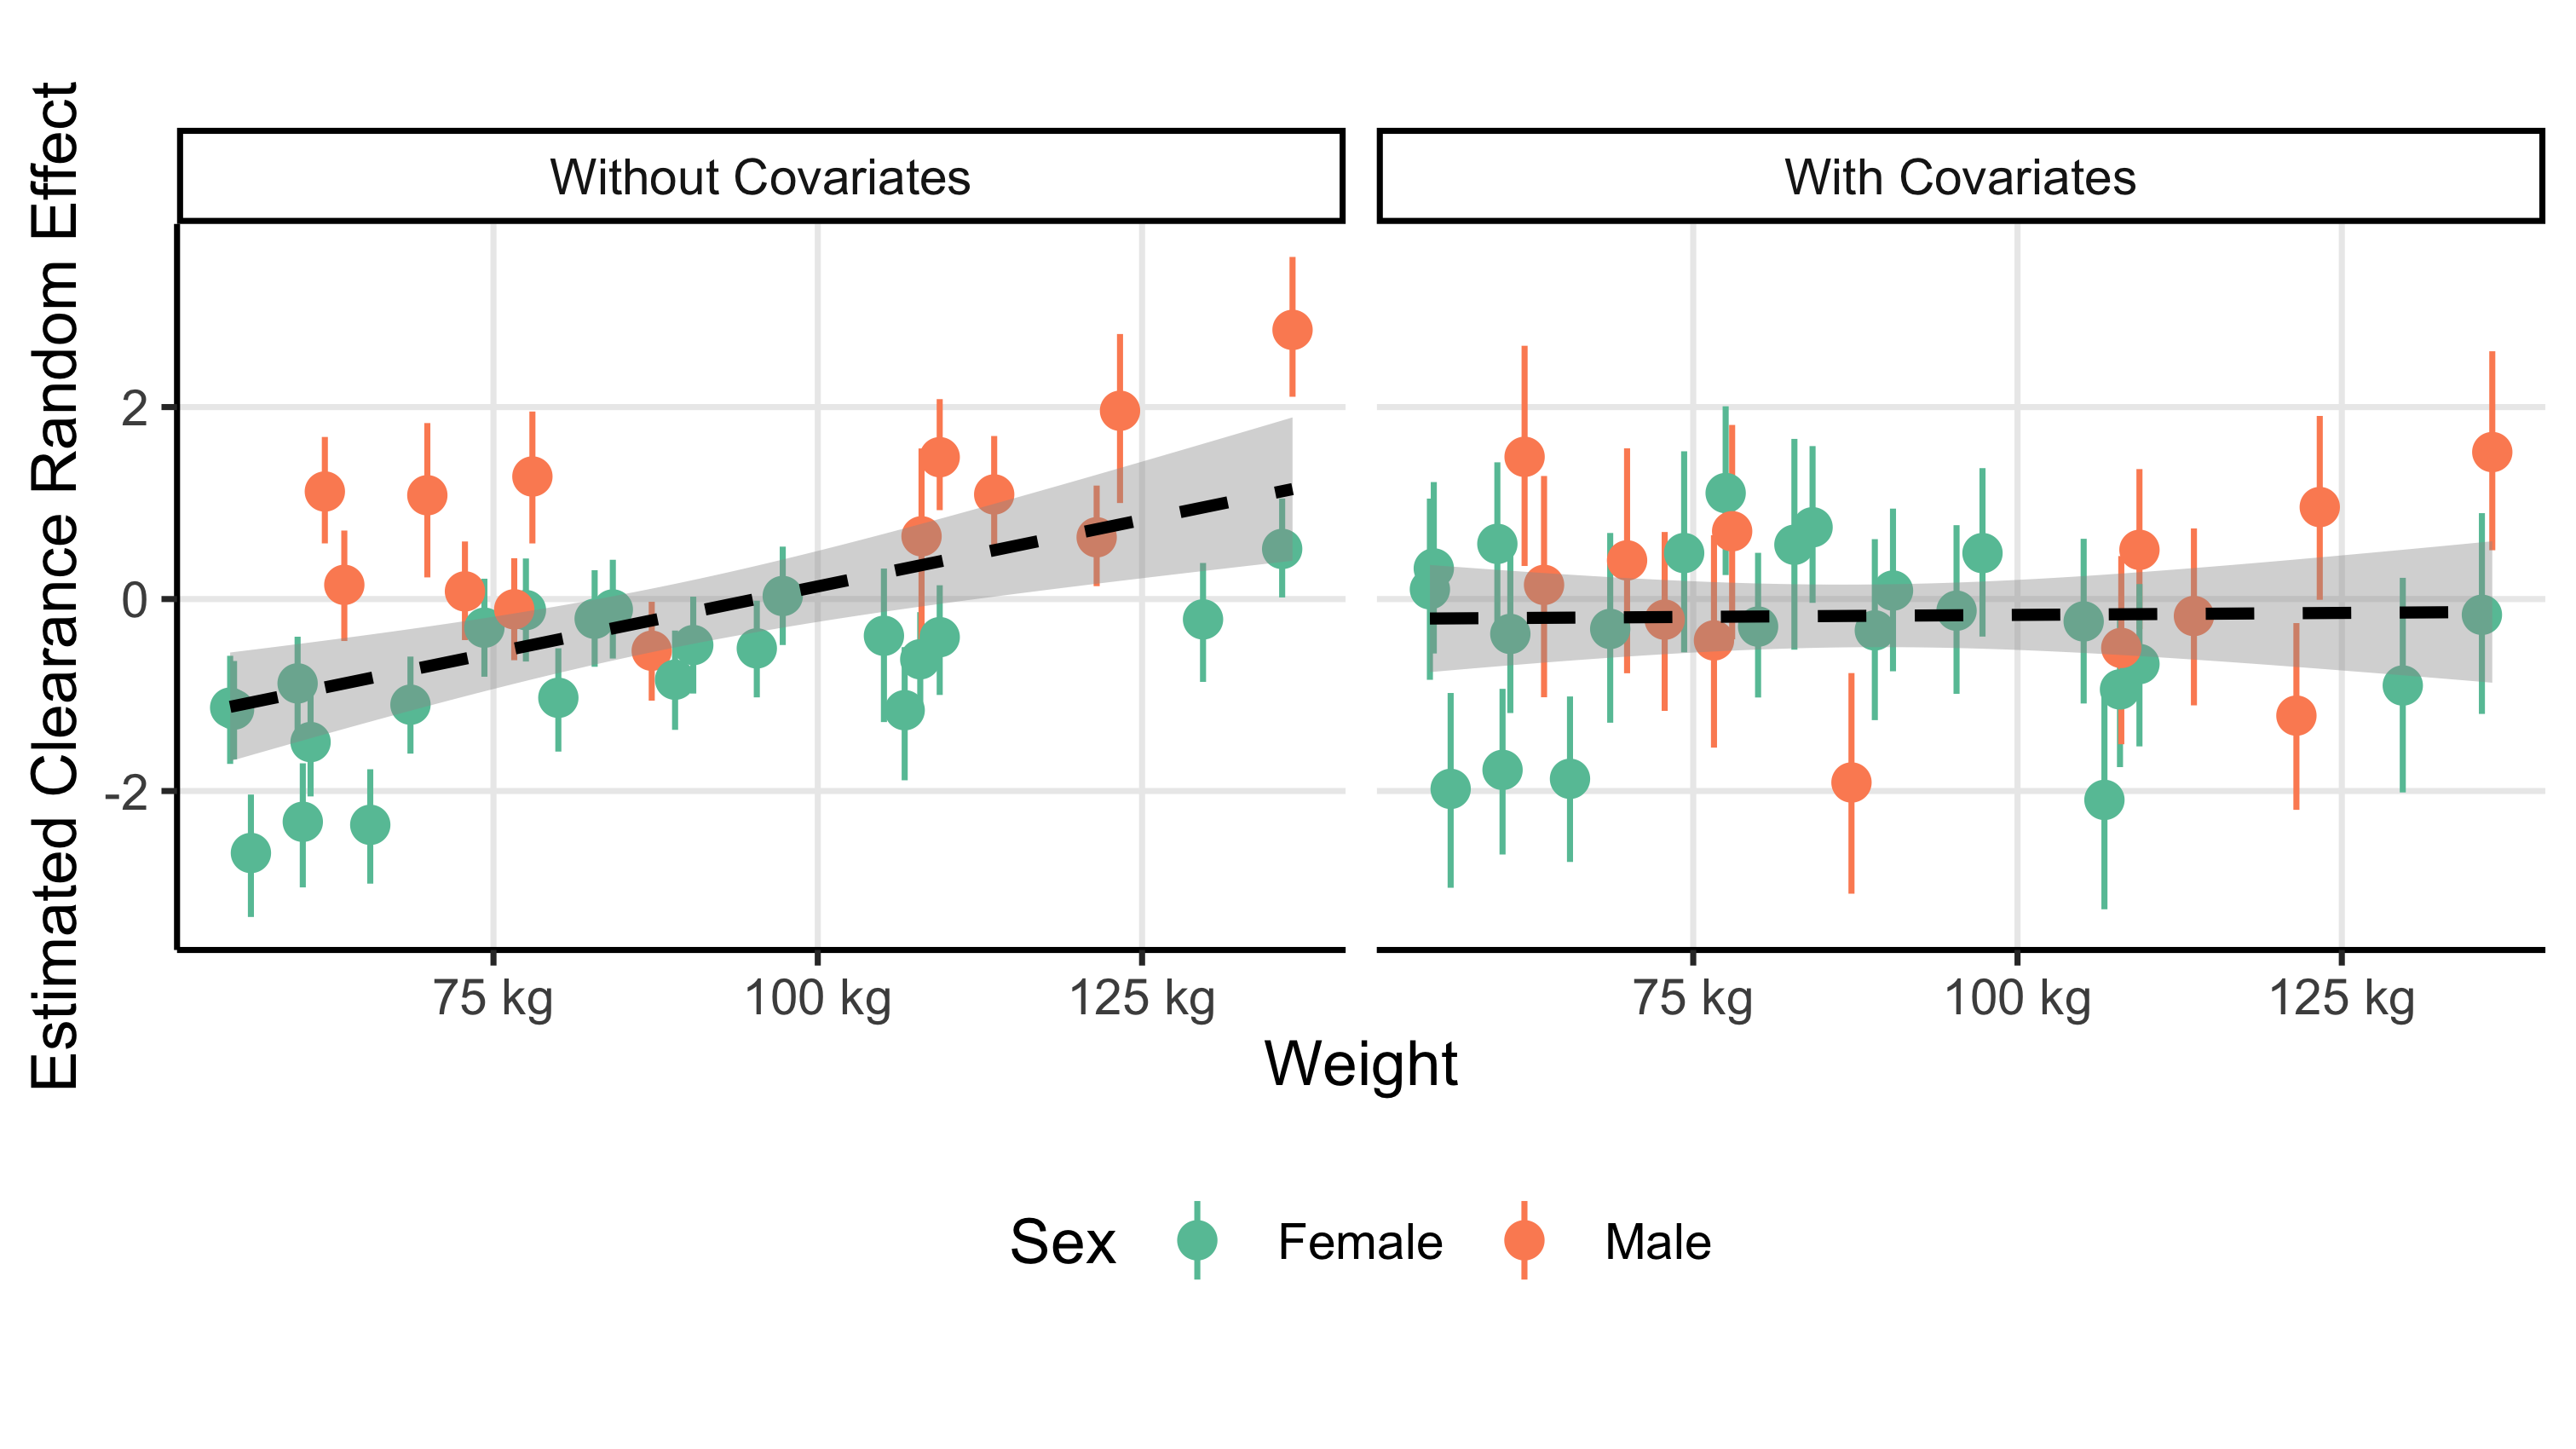
\includegraphics[width=\linewidth]{figures/random_effects_change.png}
	\caption{Random effects estimates for clearance $ \mathit{Cl}_i $ and 95\% credible intervals (left).  Random effects estimates are colored by patient sex.  Prior to adjusting for covariates, a general trend in weight can be seen in the random effects.  Patients who are heavier tend to have larger random effect, and males tend to have larger random effects than females of the same weight.  Patterns such as these indicate that weight and sex can be used to explain variation in the random effects.  After adjusting for sex and weight (right), the random effects have no discernable pattern.}
	\label{fig:randomeffectschange}
\end{figure}

We fit our model to real pharmacokinetic data using the open source probabalistic programming language, Stan \cite{gelman2015stan}.  Stan monitors several Markov chain diagnostics, none of which detected problematic Markov chain behavior, which indicates that Stan’s sampling algorithm was able to converge (0 divergences, all all Gelman-Rubin diagnostics<1.01, all effective sample sizes  > 2600).  

The inclusion of covariates in the model results in a better fit than excluding them. Shown in \cref{fig:randomeffectschange} are the estimated random effects for the clearance pharmacokinetic parameter of each patient as a function of weight.  Patient sex is indicated by color, the overall trend is shown in the black dashed line.  Failing to include patient sex and weight results in males having on average a larger random effect than females of the same weight, and heavier patients having a larger random effect than lighter patients.  When covariates are added into the model, the variation in the random effects attenuates, resulting in closer alignment to model assumptions. A better fit to the data means data generated from the model may be closer aligned with the true data generating process.

Examining the posterior distributions of the regression coefficients provides further insights into the relationships between covariates and pharmacokinetics. Greater patient weight is associated with an increase in the expected value of alpha (which is used to compute the elimination and absorption rates in the first order one compartment PK model.  The parameter $ \alpha $ is the ratio of how fast the drug exits the central compartment  how fast the drug enters the central compartment) which impacts the time to maximum concentration after each dose.  There is an estimated effect of sex on $ \alpha $ (males have smaller alpha than females, meaning the drug leaves their central compartment slower or enters the central compartment quicker), however the uncertainty is large (estimated effect -0.2 on the logit scale, 95\% credible interval -0.53 to 0.15). See \cref{tab:coefs} in the Appendix for a full summary of the regression coefficients.


%\begin{figure}
%	\centering
%	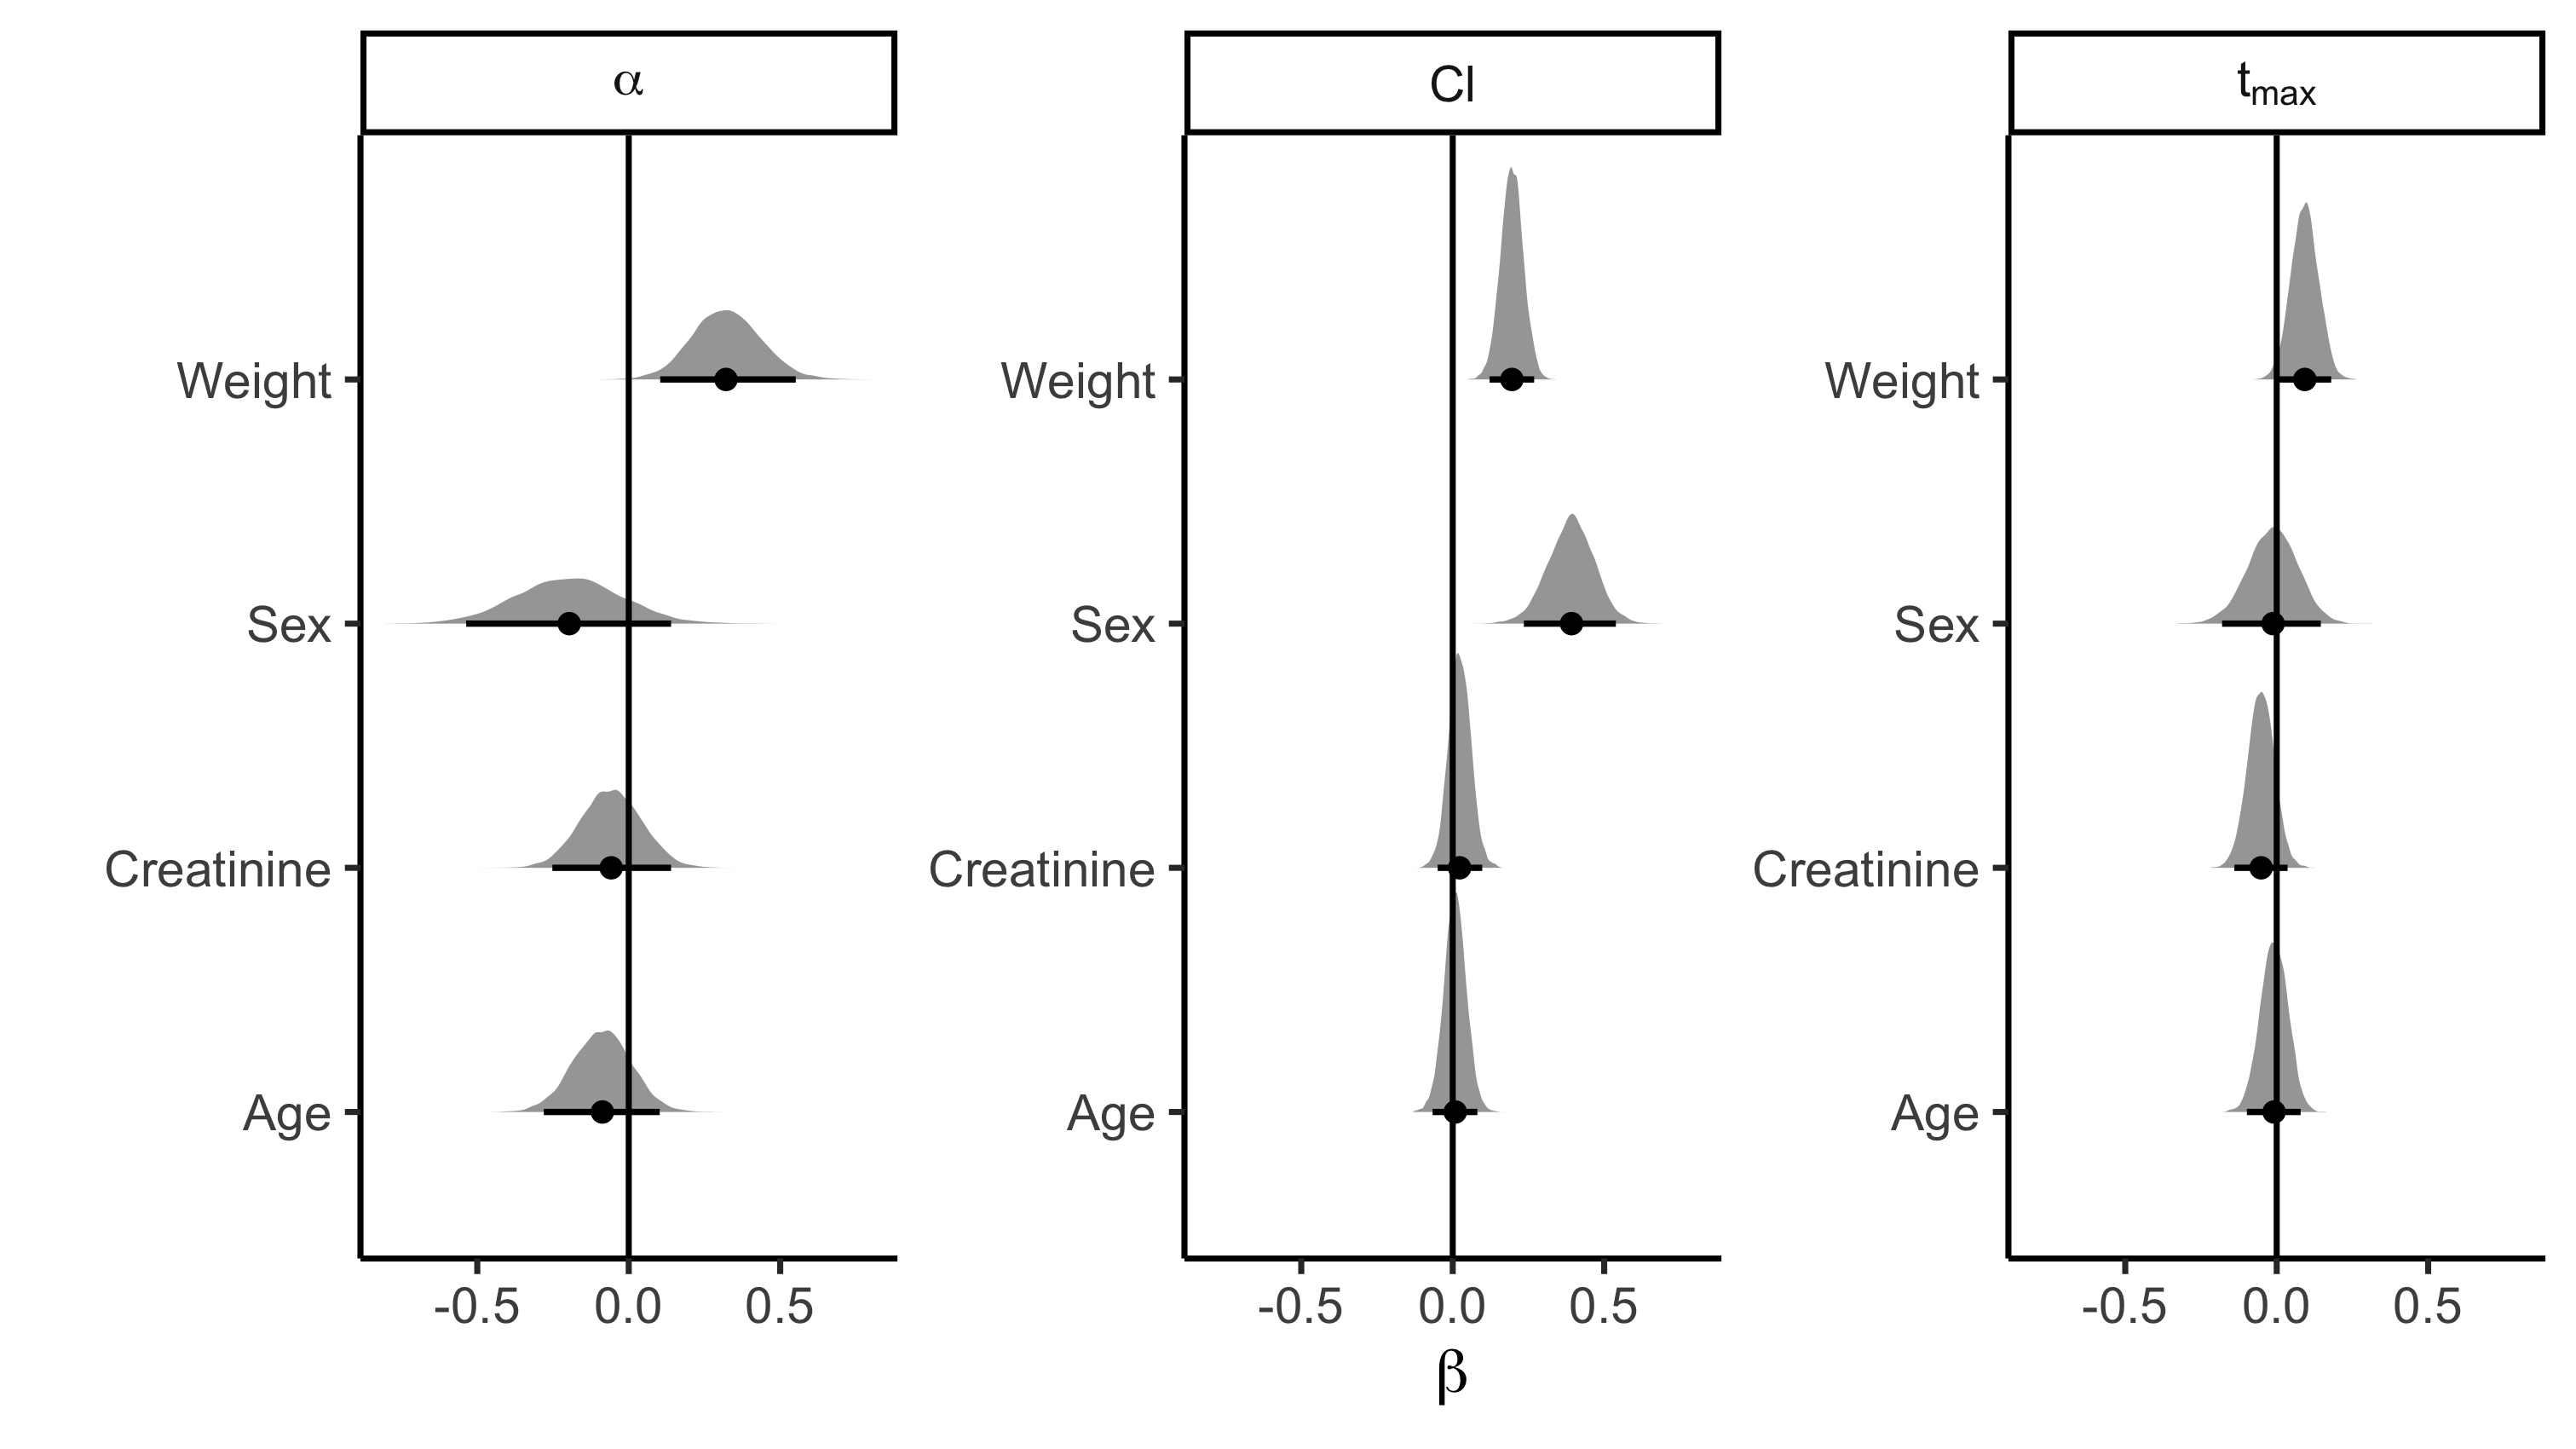
\includegraphics[width=1\linewidth]{figures/coef_vals}
%	\caption{Posterior distributions of regression coefficients. Expectations are shown as black dots, 95\% credible intervals are shown as horizontal black lines.  Solid black vertical line is $\beta=0$ for reference.  Note, regression coefficients for $\mathit{Cl}$ and $t_{max}$ act multiplicatively (a one unit increase in weight leads to a change in $\mathit{Cl}$ of $\exp(\beta)$), while regression coefficients for $\alpha$ are interpreted on the log odds scale.}
%	\label{fig:coefvals}
%\end{figure}


Model training error is comparable between the two models; the model without covariates achieves an average error of 8.31 ng/ml as measured by root mean squared error.  The model with covariates achieves a root mean squared error of 8.36  ng/ml.  Estimates of concentration uncertainty remain similar between the two models as well.  We conclude the inclusion of covariates in the model improves model inferences but does not substantially improve the fit of the model in this case.

While prediction error and concentration uncertainty are comparable between the two models, the most important differences are between inter-individual uncertainty.  The inclusion of the covariates explains variation between individual pharmacokinetic parameters, hence the between patient variability $\sigma_{\mathit{Cl}}, \sigma_{t_{max}}$ and $\sigma_\alpha$ are smaller in the covariate model as opposed to the no covariate model.  This uncertainty effects decision making, as the no covariate model is more uncertain about the pharmacokinetics of new patients.



		\chapter{Paper 3}


\section{Introduction}

One goal of personalized medicine is optimized dosing of drugs for individuals \cite{morse2015personalized}.  When considering optimal doses, a thorough understanding pharmacokinetic (what the body does to the drug) and/or pharmacodynamic (what the drug does to the body) effects are crucial.  To this end, models describing the mediation of pharmacokinetic/pharmacodynamic effects via clinical, genetic, and lifestyle factors have an important role in deciding which patients should get what dose. Models of this nature are sometimes published by research teams collaborating with drug manufacturers using data from clinical trials.

Independent investigators can find themselves in a situation in which data collection from a particular population of interest is achievable. If the data come from practice (e.g. a personalized medical clinic), there may be questions about how new variables not previously studied in clinical trials affect the pharmacokientics/pharamcodynamics of a particular drug.  Running large studies in order to examine the effects of these new variables, or discover effects of other variables, may be unrealistic due to a variety of constraints.  Consequently, investigators must think about how best to model the pharmacokinetics, for use in decision making \textit{and} exploration, using the data available to them.

The oral anti-coagulant apixaban provides an illustrative example.  Pharmacokinetic models have been previously published \cite{cirincione2018population,ueshima2018population} in collaboration with the drug's manufacturer using data from clinical trials.  These studies identified age, sex, body weight, renal function,  patient race, and CYP3A4 inhibitors as modulators of apixaban pharmacokinetics \cite{cirincione2018population}, though according to authors the effects of some of these variables were not large enough to require clinical dose adjustment. However, even after adjusting for the aforementioned factors, concentrations of apixaban in real life applications have been observed to be larger than what was reported in clinical trials \cite{sukumar2019apixaban}, raising questions as to the optimal dosing of apixaban for patients in different settings. Additionally, recent research has indicated appropriateness of dose adjustment criteria are unclear \cite{vu2021critical}, citing there is no reduction in safety associated with an increased exposure to apixaban in patients above 75 years of age, below 60kg of body weight, and EGFR lower than 50 mL/min. The uncertainty regarding dosing criteria and additional variability in concentrations in day to day use suggests that, while previously published models may be internally valid, these models may not be representative of all populations in which apixaban is to be applied.  That is to say, the models may lack a degree of external validity, thus supporting the idea that pharmacokinetic models may need to be tailored for specific populations of interest. When viewed through a Bayesian lens, the previous modeling work can act as an informative prior on various pharmacokinetic/pharmacodynamic measures.  Creating new models for populations of interest is then more of a "fine tuning" than an all together new approach.  Pharmacokinetic models for use in a specific population may then have two goals:  to adjust doses for a specific population, and/or to explore how additional variables (for example, concomitant medications) not included in the previous studies affect particular parts of the pharmacokinetics of apixaban.  

This study seeks to demonstrate how investigators can fit similar models to their pharmacokinetic data with the aim of accomplishing the goals of accurate modeling of pharmacokientics and exploration of effects of new variables.  We use apixaban as a specific example, but our methodology can be generalized to other drugs for which pharmacokientics are of interest.  Importantly, we only focus on pharmacokientics since blood plasma levels correlate closely with the pharmacodynamic effect of apixaban \cite{byon2019apixaban, upreti2013effect, frost2013safety,frost2013apixaban}. Our approach leverages a Bayesian methodology to building pharmacokinetic models so that we may incorporate prior information from previous studies. Additionally, we describe how investigators can use \textit{all} relevant data available to them to fit these models and make inferences, even if the data are not from controlled studies.  Also, we show how sparsity inducing priors can be applied to new variables in order to explore how those variables may effect apixaban pharmacokinetics, encouraging negligible effect sizes but allowing for large effects to be detected at the cost of a small amount of bias. We present a small simulation study to demonstrate how smallest meaningful effects can be detected through these priors as a function of sample size. Finally, we use an open source Bayesian language to develop our models, making our code freely available.  Previous models are constructed in a proprietary software tool set, which can present a barrier for some. Creation of these models in a free tool removes a barrier to research, making these methods more widely available.

		\section{Background}

\subsection{Apixaban}

Apixaban is a direct acting oral anti-coagulant often prescribed for prevention of stroke and systemic embolism in patients with atrial fibrillation (AF) \cite{BMSmonograph,byon2019apixaban}.  Studies as recent as 2019 have reported excess variability in observed apixaban plasma concentrations in patients with AF \cite{sukumar2019apixaban}. Since apixaban plasma concentrations correlate closely with anti-coagulation, excess variability in these concentrations may mean increased risk of bleeding. These findings have raised questions towards the optimal dosing of apixaban in older adults with AF encountered outside of clinical trials. Additional research into determining factors which explain this excess variability beyond known clinical factors \cite{gulilat2020drug} has consequently begun.

\subsection{Variable Selection}


Existing studies into pharmacokinetic modelling often use variable selection methods (e.g. variants of stepwise selection, including fitting all submodels \cite{cirincione2018population,ueshima2018population}) when faced with the determining which variables effect the pharmacokientics. Many studies have noted that these techniques result in bias away from the null \cite{whittingham2006we}, exaggerated precision \cite{altman1989bootstrap}, inaccurate or uninterpretable $p-$values due to inability to properly incorporate uncertainty in the selection process \cite{harrell2015regression}, and can fail to select the "true" model with high confidence even when modelling assumptions are consistent with the true data generating process \cite{smith2018step}.  Hence, even in the best case scenario where the selection procedure identifies the correct variables, the resulting estimates may not be reliable.  Results from these studies methods make a convincing argument to avoid selection methods all together.

Variable selection methods are intended to answer the question "which variables are important in modelling the outcome", and although studies have demonstrated deficiencies with variable selection, they often do not provide an alternative answer.  From a Bayesian perspective, selection to include a variable in or out of a model defines a sort of prior on the parameter value; there is a strong preference for a null effect estimate unless the data provide sufficient evidence for free estimation of that effect.  Efforts to operationalize this prior structure in terms of Bayesian inference have lead to a wide variety of sparsity inducing priors, which include spike and slab priors \cite{mitchell1988bayesian}, and horseshoe \cite{carvalho2010horseshoe} and Finnish horseshoe priors \cite{piironen2017sparsity}. These approaches admit that while unlikely that the effects of unimportant variables are exactly 0, they may be small enough to be negligible.  These priors place the majority of their probability mass near 0, encouraging small effects to be estimated as something negligibly small, but allow for large effects to be identified at the cost of a small amount of bias.

Bias towards a null effect  can be acceptable when the goal is exploration and prediction.  The bias can act as a regularization for predictions hence combating overfitting, and can hedge estimates of novel effects when they are exaggerated due to high variance. To this end, we present a simulation study in which we use a sparsity inducing prior to estimate the effect of a concomitant medication on apixaban pharmacokinetics.  In particular, the medication is assumed to inhibit a particular gene important in the elimination of apixaban, making the bioavailability larger.  We place a double exponential (or Laplace) prior on the effect of the concomitant medication, as well as a prior on the parameter for the Laplace distribution.  This is similar to putting a LASSO penalty on the effect as well as a prior on the LASSO penalty strength \cite{tibshirani1996regression}.  Although our simulation only has a single variable of interest, many variables can be used with this prior structure.

For our simulation, we generate data from the posterior of a previously fit model. We simulate 10 datasets from a pre-specified number of repeatedly sampled patients (we examine 5, 10, 20, 30, 40, and 50 repeatedly sampled patients) haven taken their first dose of the drug with a pre-specified and fixed effect of a concomitant medication on the bio-availability of the drug.  We assume that investigators can sparsely sample patients more easily, and so we simulate 10 times more sparsely sampled patients who have already achieved steady state. We do this so as to more closely resemble real life scenarios in which patients come into a clinic for a plasma measurement having already been on the drug for sometime. We examine effects of 0, 0.125, 0.25, 0.5, 1.0, and 1.5 on the logit scale (we use the logit scale since bioavailability is constrained to be between 0 and 1). 

\subsection{Why Is a Hierarchical Model Needed?}

In this paper, we propose a pooling of both sparsely and repeatedly sampled data in a single model. Pooling information is not a new approach, and reasonable arguments could be made to use simpler models.  After all, if the sparsely sampled data models a continuous outcome as a function of covariates, why would investigators use a complex model when something simple like linear regression (or linear regression on log concentrations) may be sufficient?  While simpler approaches and criticisms of using unnecessarily complex models are valid, both linear modelling and mixed effects models for pooling suffer from important drawbacks in the case when attempting to combine sparsely sampled and repeatedly sampled data from different studies.  We examine those drawbacks below.

Linear regression can be, and has been \cite{gulilat2020drug,vakkalagadda2016effect}, used to model apixaban concentrations as a function of time and other covariates using sparsely sampled data.  When certain criteria are met, there is good reason to do so.  The concentration profile, $C(t)$, from a first order absorption with linear elimination pharmacokinetic model looks like

$$ C(t) = \frac{F \cdot D}{C l} \frac{k_{e} \cdot k_{a}}{k_{e}-k_{a}}\left(e^{-k_{a}t}-e^{-k_{e}t}\right) $$

\noindent Here, it is usually assumed that $k_e<k_a$ in order for the model to be identified \cite{wakefield1996bayesian, salway2008gamma}. The elimination phase occurs when $t$ is sufficiently large, resulting in $C(t)$ being approximately exponential and $\log(C(t))$ being linear in time on the log scale with slope $-k_e$.  The assumption that measurement error is additive on the log scale facilitates use of linear regression.

This approach is common in pharmacokinetics when estimating the elimination rate but suffers from three important drawbacks generally. First, the elimination rate is not allowed to vary as a function of known factors which effect elimination rate, such as kidney function.  This can be ameliorated by specifying an interaction between time and those covariates known to effect elimination rate (though this has not been done in all studies \cite{gulilat2020drug}).  Second, an exponential approximation is only appropriate when time is sufficiently large.  Clearly, the exponential approximation breaks down near $t=t_{max} = \log(k_a/k_e)/(k_a-k_e)$ and is completely inappropriate in the absorption phase when $t<t_{\max}$.  This affects estimates of max concentration in an appreciable way, resulting in an upward bias of $C_{\max}$ (the bias is proportional to $-k_a t_{\max}$ on the log scale).  Additionally, because $t_{\max}$ is not modelled per individual, estimates of $C_{\max}$ must rely on a point estimate of $t_{\max}$.  This results in uncertainty estimates of $C_{\max}$ which may be too narrow for a given individual.  Finally, the effects of covariates on other aspects of the pharmacokinetcs are undetermined. Assuming a linear model is used to model concentrations on the log scale, we find

\begin{align}
	\log(C(t)) & = \log(D) + \log(F) - \log(Cl) + \log(k_e) + \log(k_a) - \log(k_e-k_a) + \log\Big( e^{-k_{a}t}-e^{-k_{e}t} \Big) \nonumber \\
	                 & \approx \log(D) + \beta_0 + \beta_1t \qquad \mbox{when  } t_{\max} \ll t \>. \nonumber
\end{align}


\noindent Here, $\beta_0 =  \log(F) - \log(Cl) + \log(k_e) + \log(k_a) - \log(k_e-k_a)$.  If covariates are included in the model, then although changes in log concentration may be accurate (in so far as the sign of the chance in log concentration is concerned), \textit{where that change occurs is under determined}.  Did concentration increase because bioavailability ($F$ in the log linear model) increased, or was it because the clearance rate ($Cl$ in the log linear model) decreased?  We can't say for certain from this model. In order to determine if a change in concentration was due to an increase/decrease in a pharmacokinetic parameter, each pharamacokinetic parameter must be modeled as functions of covariates. How salient these drawbacks are is up to the investigator, but if any of them are important to decision making for personalized medicine then a linear model will not be appropriate.

Mixed effects models can be used to pool information from many datasets.  Meta-analysis is perhaps the most prevalent example of this approach.  A typical example may be pooling data from studies conducted using similar protocols across multiple centers.  Ideally, the data are collected under similar protocols, making assumptions regarding the likelihood and exchangeability of appropriate units tenable.  In the scenario we describe, where information from at least two studies with different protocols are to be pooled, we believe a mixed effect model specifying between study variation is *not* appropriate due to subjects not being exchangeable between studies.  Recall, a sequence of random variables $\theta_1, \dots, \theta_n$ is said to be exchangeable in their joint density $p(\theta_1, \dots, \theta_n)$ is invariant permutations of the indicies $(1, \dots, n)$ \cite{gelman1995bayesian}.  If no other information, other than observed data, is available to distinguish any of the $\theta_j$ from any others, and no ordering or grouping of parameters can be made, one must assume exchageability of the $\theta$.  In the scenarios we describe, we do have additional information which can be used to distinguish the $\theta$.  In particular, sparsely sampled data will have a larger estimated residual error than repeatedly sampled data.  This is because the residual variance is a combination of within and between subject variation. There are then 2 residual variances to be estimated: one for the repeatedly sampled data and one for the sparsely sampled data.  When pooling sparsely sampled and repeatedly sampled data together, individuals within subjects are exchangeable because of the common residual variance within study. However, subjects are not exchangeable between studies because permutations of the subject indicies fail to account for which subject should be associated with which residual error.
		\section{Bayesian Model}


Our model specifies a population level effect of covariates (age, sex, weight (kg), serum creatinine ($\mu \mbox{mol}$)) on patient clearance, time to max concentration, and the ratio between absorption and elimination rates (a unitless parameter we refer to as $\alpha$). These effects are shared between all populations, allowing information from one dataset to partially inform model fit on the other.  We also include a population level effect of concomitant amiodarone on bioavailability of apixaban.  We fit our model using Stan [-@gelman2015stan], an open source probabilistic programming language with interfaces to Python, R, Stata, Matlab, and more.

Let $s = 1 \dots K$ denote the number of studies being pooled together.  Each study has $j = 1 \dots N_s$ subjects, whom are observed at times $t_i$ for $i = 1 \dots T_j$.  For sparsely sampled data, $T_j=1$, meaning we have only one sample per subject.  For repeatedly sampled data, $1<T_j$, meaning we have multiple measurements from the same subject.  In our data, we use $K=2$ studies.  There are $N_1=36$ subjects in our repeatedly sampled data, and $N_2=402$ subjects in our sparsely sampled data.  The repeatedly sampled subjects are each sampled $T=8$ times.

Our model assumes there are population level effects of each covariate on the pharmacokientic parameters, and that the distribution of pharmacokinetic parameters given covariates $\mathbf{x}_{j, s}$ from subject $j$ in study $s$ are the same between studies.  Let $\theta_{j, s}$ be a vector of pharmacokinetic parameters for subject $j$ in study $s$.  In our model, $\theta_{j, s}$ is comprised of subject clearance rate, time to max concentration, ratio between elimination and absorption rates, and bioavaiability respectively  $\theta_{j,s} = (Cl_{j, s}, t_{\max, j, s}, \alpha_{j, s}, F_{j, s})$.  Our model is depicted as a Bayes net in Figure 1.

We estimate two non-pharmacokientic parameters from our data as well.  Let $\delta_{j, s}$ be the time delay between ingestion of the bolus dose and absorption into the blood stream, and let $c_{0, j, s}$ be the initial concentration of apixaban in the blood stream at the time of ingestion.  The time delay $\delta$ can not be estimated from the sparsely sampled data because only a single measurement was taken, but can be estimated from the repeatedly sampled data.  Therefore we assume $\delta_{j, 2}=0 \quad \forall j$.  Additionally, sparsely sampled patients are assumed to be in steady state and therefore have a non-zero initial concentration of apixaban in their blood at the time of ingestion, as compared to repeatedly sampled patients which had not taken apixaban prior to the study.  Therefore, $c_{0, j, 1} = 0 \quad \forall j$.  The quantity $c_{0, j , 2}$ can be estimated from the other pharmacokinetic parameters assuming subjects have been taking apixaban twice daily with perfect adherence for the last 5 days.  We provide a proof of this proposition in the appendix by solving the associated differential equation with forcing functions for each dose using the Laplace Transform.

Each pharmacokinetic parameter has an associated set of regression coefficients and intercept term.  Each pharmacokinetic parameter is regressed on subject covariates $\mathbf{x}_{j, s}$ in the following way:
\begin{align}
 \log(Cl_{j, s}) &= \mu_{Cl} + \mathbf{x}_{j, s}^{Cl} \beta_{Cl}\\
 \log(t_{\max,j, s}) &= \mu_{t} + \mathbf{x}_{j, s}^{t} \beta_{t} \\
 \operatorname{logit}(\alpha_{j, s}) &= \mu_{\alpha} + \mathbf{x}_{j, s}^\alpha \beta_{\alpha}\\
 \operatorname{logit}(F_{j, s}) &= \mu_{F} + \mathbf{x}_{j, s}^{F} \beta_{F}
\end{align}





Here, we have added superscripts to the $\mathbf{x}$ to indicate that different covariates may be used in each regression. The $\beta$ are regression coefficients and $\mu$ are intercepts for the parameter indicated in the subscript. We include random effects for repeatedly sampled subjects. Each $\theta_{j, s}$ is used to predict the concentration profile $C(t)$.  We use a one compartment pharmacokinetic model with first order elimination as our $C(t)$, namely

$$ C_{j, s}(t_i) =  \begin{cases} c_{0, j, s} + \dfrac{D_{j, s} F_{j, s} k_{e, j, s} k_{a, j, s}}{Cl_{j, s}(k_{e, j, s} - k_{a, j, s})} \Bigg( e^{-k_{a, j, s}(t_i - \delta_{j, s})} - e^{-k_{e, j, s}(t_i - \delta_{j, s})} \Bigg)  & \delta_{j, s} \leq t_i \\ 0 & \mbox{else} \end{cases}$$

Again, if $s=1$ (indicating repeated sampling) then $c_{0, j, 1} = 0 \quad \forall j$ since patients from this study take apixaban for the first time.  If $s=2$ (indicating sparse sampling) then $\delta_{j, 2}$ is assumed to be 0 $\forall j$ since the delay can not be estimated from a single observation.  Finally, the predicted latent concentrations are used in the likelihood.  We use a lognormal likelihood for both datasets, with variance differing by study

$$ y_{i,j,s} \sim \operatorname{Lognormal}\Big( \log(C_{j, s}(t_i)), \sigma_s \Big)  \>.$$


\begin{figure}[t!]
	
	\centering
	\begin{tikzpicture}
		
		\node[latent](b){$\beta$};
		\node[latent, right=of b](mu){$\mu$};
		
		\node[latent, below = of b](theta){$\theta$};
		\node[obs, left = of theta](x){$\mathbf{x}$};
		
		
		\node[latent, below = of theta](C){$C(t)$};
		\node[obs, left = of C](t){$t$};
		\node[obs, below = of C](y){$y$};
		\node[latent, left = of y, xshift=-2cm](s){$\sigma$};
		
		\edge{b}{theta};
		\edge{mu}{theta};
		\edge{x}{theta};
		\edge{theta}{C};
		\edge{t}{C};
		\edge{C}{y};
		\edge{s}{y};
		
		\plate[]{t_y_pairs}{(t)(y)(C)}{$i=1 \dots T_j$};
		\plate[]{subjects}{(t_y_pairs)(x)(theta)}{$j=1 \dots N_s$};
		\plate[]{study}{(subjects)(s)}{$s=1 \dots K$};
	\end{tikzpicture}
	\caption{Bayes net for our hierarchical apixaban pharmacokientics model.  Here, $\beta$ and $\mu$ are regression coefficients and intercepts for the effects of covariates on pharmacokientic parameters.  The effects are assumed to apply to all studies, meaning that the effect of age on time to max concentration (as an example) is the same for all studies.  If protocols are different between studies, then each study may have a different residual variance term $\sigma_s$.  This differing residual variance is what prevents subjects from being considered exchangeable between studies.  When permuting the joint distribution of $\theta_{j, s}$, one needs to keep track of which $\theta$ requires which $\sigma$, thus preventing the subjects from being considered exchangeable.}
\end{figure}


		\section{Results}

The results from our simulation study are shown in figure \ref{fig:simulation-results}. The precision of the estimate of effect of concomitant drug use increases as the number of repeatedly sampled (and sparsely sampled) patients increases.  Shown in red are the sample means of the 10 runs (black dots).  On average we see a small amount of bias in the estimates.  This is expected since the sparsity inducing priors have the majority of their density in a small neighbourhood of 0, regularizing effects towards 0.  For purposes of discovery, these biases may be acceptable if the result is a decrease in model variability.



\begin{table}
	
	\caption{\label{tab:table-1}Descriptive statistics for repeatedly sampled and sparsely sampled data.  Note, amiodarone is a CYP3A4 inhibitor.  The study which generated repeatedly sampled data excluded any patients whom were taking CYP3A4 inhibitors, so all patients in the repeatedly sampled data are assigned a value of 0 for concomitant amiodarone.}
	\centering
	\begin{tabular}[t]{llll}
		\toprule
		& Repeatedly Sampled Data & Sparsely Sampled Data & Overall\\
		\midrule
		& (N=36) & (N=401) & (N=437)\\
		\addlinespace[0.3em]
		\multicolumn{4}{l}{\textbf{Age}}\\
		\hspace{1em}Mean (SD) & 49.8 (11.5) & 78.8 (9.43) & 76.4 (12.5)\\
		\hspace{1em}Median [Min, Max] & 50.0 [26.0, 70.0] & 79.0 [47.0, 98.0] & 79.0 [26.0, 98.0]\\
		\addlinespace[0.3em]
		\multicolumn{4}{l}{\textbf{Weight (kg)}}\\
		\hspace{1em}Mean (SD) & 88.0 (24.4) & 85.6 (23.8) & 85.8 (23.8)\\
		\hspace{1em}Median [Min, Max] & 83.5 [54.7, 137] & 81.6 [40.0, 221] & 81.8 [40.0, 221]\\
		\addlinespace[0.3em]
		\multicolumn{4}{l}{\textbf{Creatinine (micromol/L)}}\\
		\hspace{1em}Mean (SD) & 68.0 (12.5) & 105 (44.5) & 102 (43.9)\\
		\hspace{1em}Median [Min, Max] & 65.0 [50.0, 95.0] & 92.0 [42.0, 316] & 89.0 [42.0, 316]\\
		\addlinespace[0.3em]
		\multicolumn{4}{l}{\textbf{Sex}}\\
		\hspace{1em}female & 23 (63.9\%) & 178 (44.4\%) & 201 (46.0\%)\\
		\hspace{1em}male & 13 (36.1\%) & 223 (55.6\%) & 236 (54.0\%)\\
		\addlinespace[0.3em]
		\multicolumn{4}{l}{\textbf{Concomitant Amiodrone (mg/day)}}\\
		\hspace{1em}Mean (SD) & 0 (0) & 16.2 (60.1) & 14.9 (57.7)\\
		\hspace{1em}Median [Min, Max] & 0 [0, 0] & 0 [0, 400] & 0 [0, 400]\\
		\bottomrule
	\end{tabular}
\end{table}


\begin{figure}
	
	{\centering 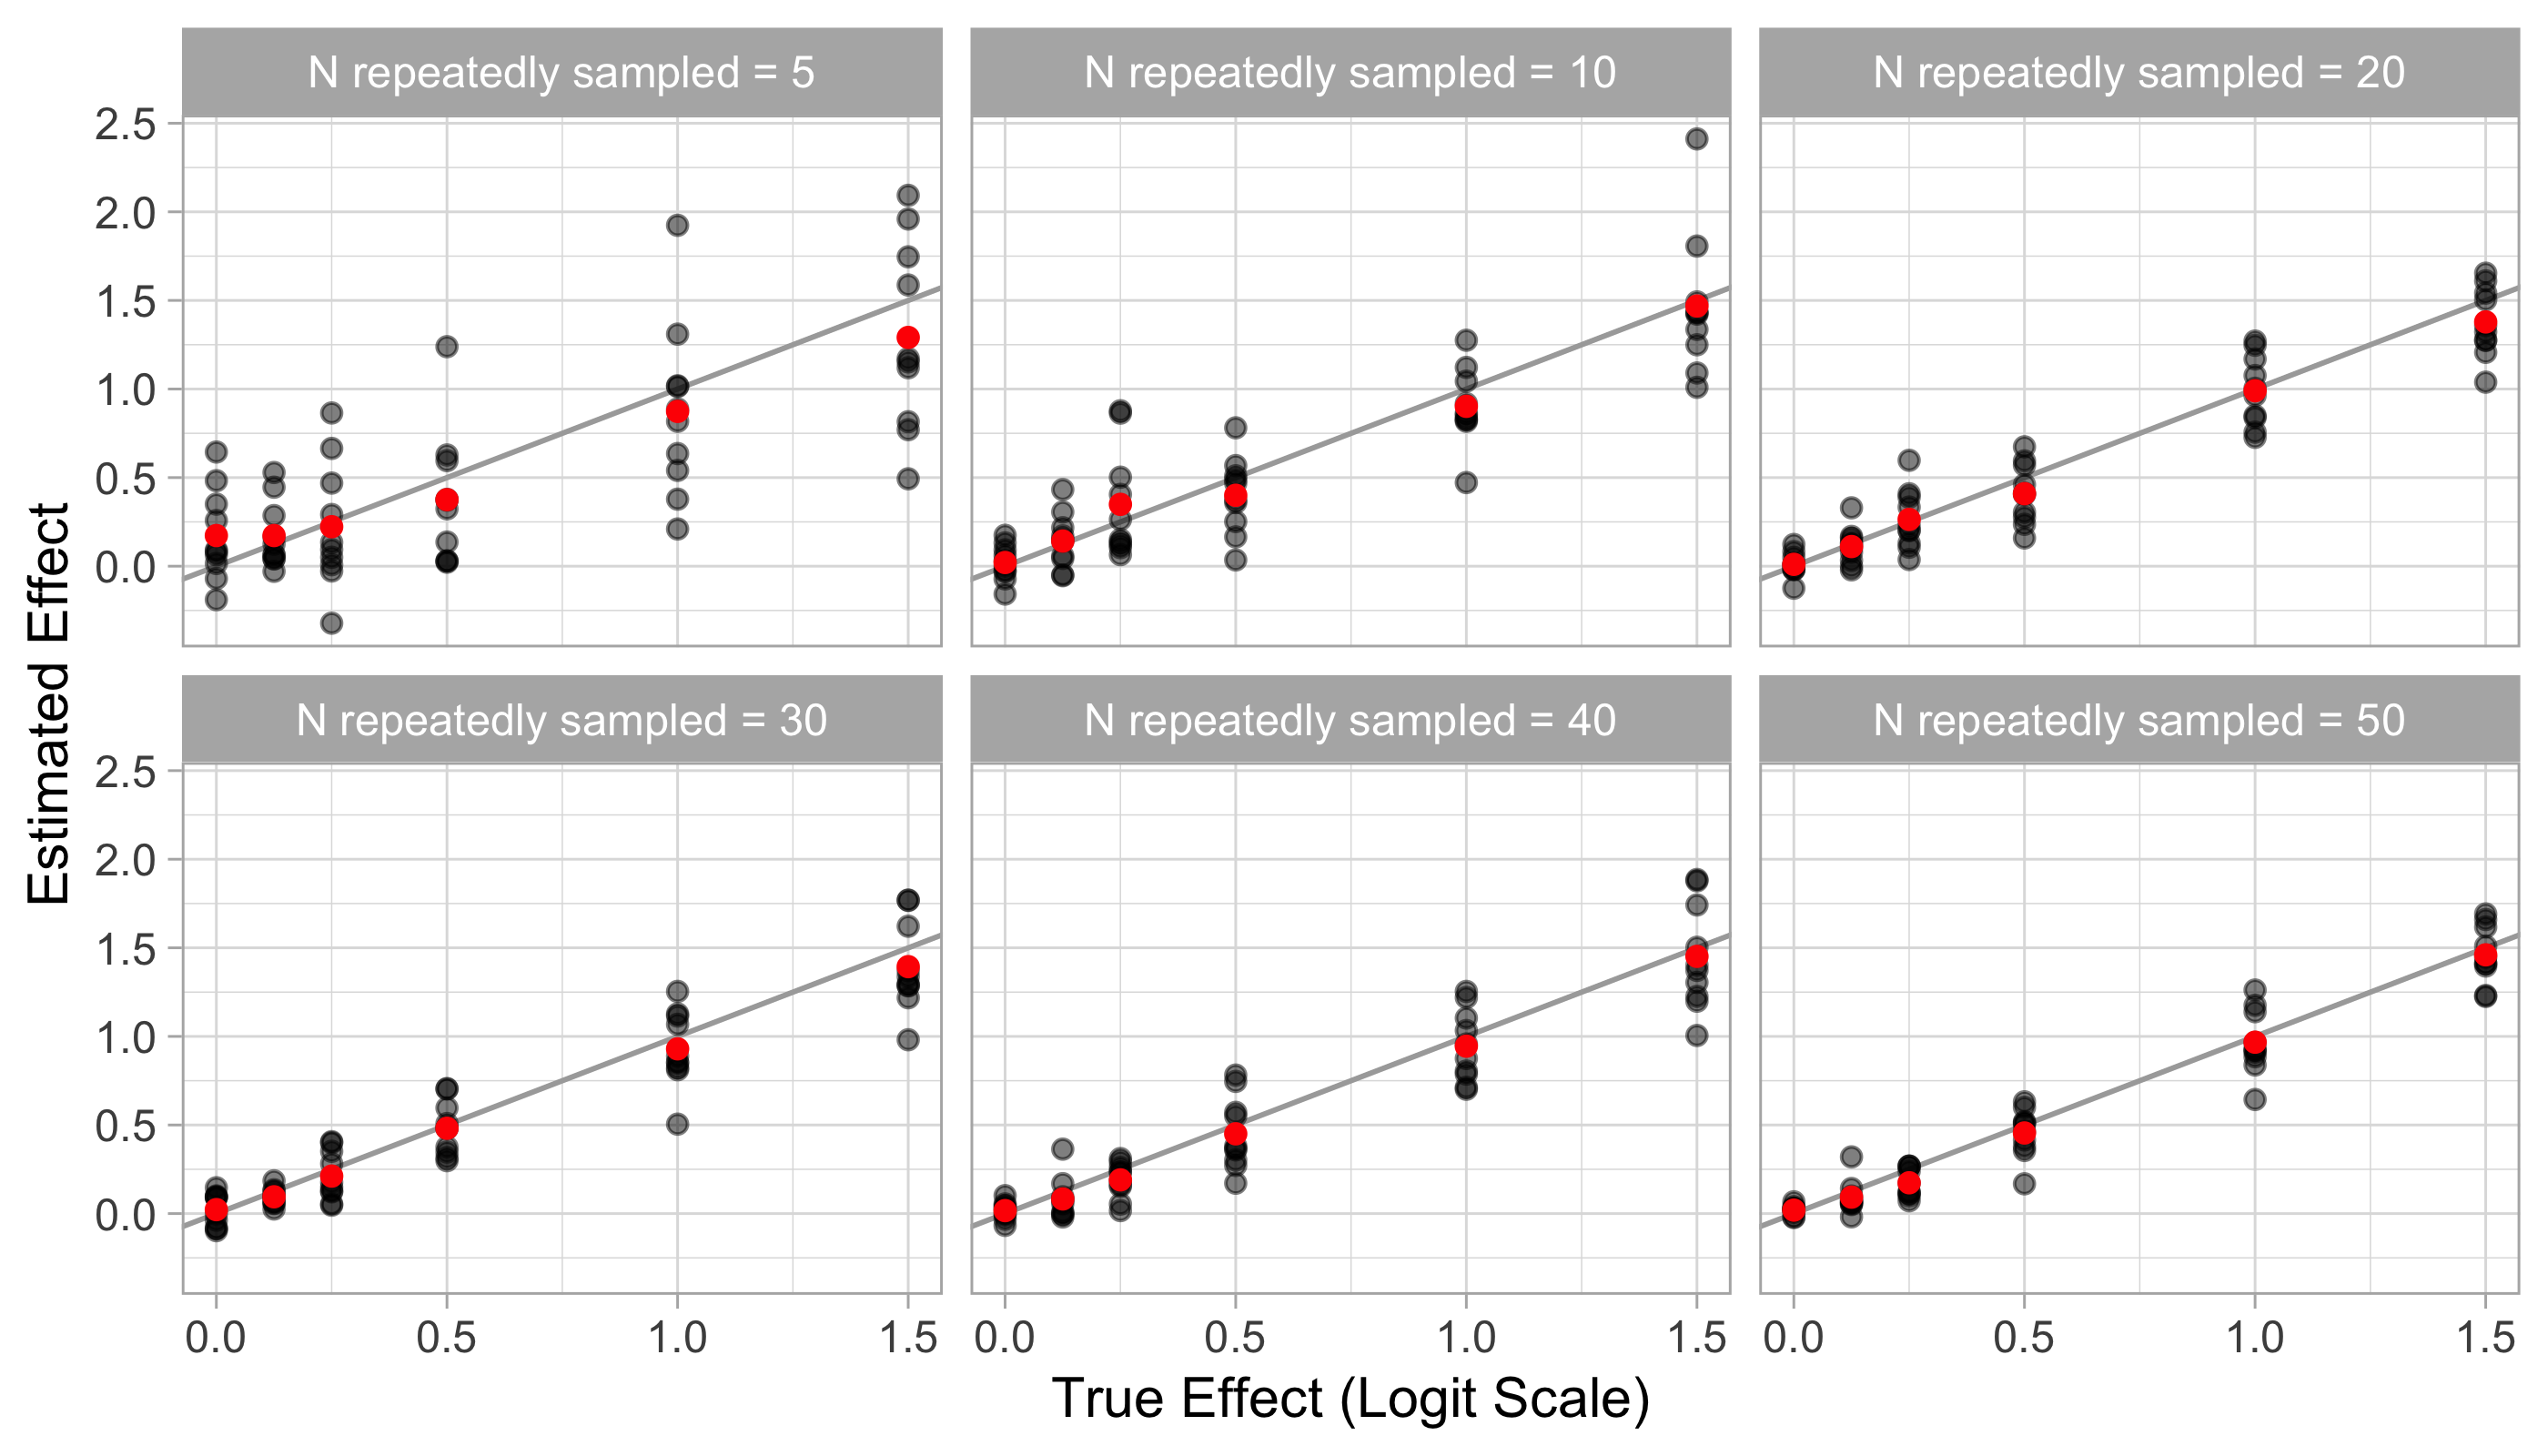
\includegraphics[width=\linewidth]{figures/simulation-results-1} 
		
	}
	
	\caption{Results from our simulation study.  Black dots represent the estimated effect of a novel predictor.  Red dots indicate the average estimate across the 10 repetitions. Data are faceted by the number of repeatedly sampled patients.  Smaller datasets show more bias towards the null.  This bias attenuates as sample size increases.}\label{fig:simulation-results}
\end{figure}


When using real data, our model can accurately predict both repeatedly
sampled and sparsely sampled data. Shown in figure
\ref{fig:plot-model-predictions} is a log-log plot of predicted and
actual concentrations for both datasets. The model makes more accurate
predictions for repeatedly sampled patients (because it is able to
estimate the random effect in each pharmacokinetic parameter). The
apparent increase in prediction error for the sparsely sampled can be partially
explained by the absence of random effects for each patient. The within
and between patient variation manifests as measurement error solely,
thus leading to lower predictive ability.

With a model for the pharmacokinetics of apixaban in hand, estimates of
salient pharmacokinetic phenomena can be easily obtained. In figure
\ref{fig:max-concentration}, we use our model to estimate the max
concentration for the reference patient under different doses of
amiodarone. Through our model, we estimate concomitant amiodarone
increases bioavailability, which in turn increases max concentration.
Shown in black is the expected max concentration conditioned on
concomitant amiodarone dose, as well as 95\% equal tailed posterior
credible intervals.

Additionally, we contrast the pooled model's estimates of covariate
effects with estimates from model's fit to either the sparse or
repeatedly sampled data. Marginal posterior densities for the effects of
covariates on the pharmacokientic parameters are shown in figure
\ref{fig:effect-estimates}. In most cases, the effects seem to have
higher precision due to the increase in sample size, and generally there
is no large disagreement in either sign or magnitude of effect
estimates.



\begin{figure}
	
	{\centering 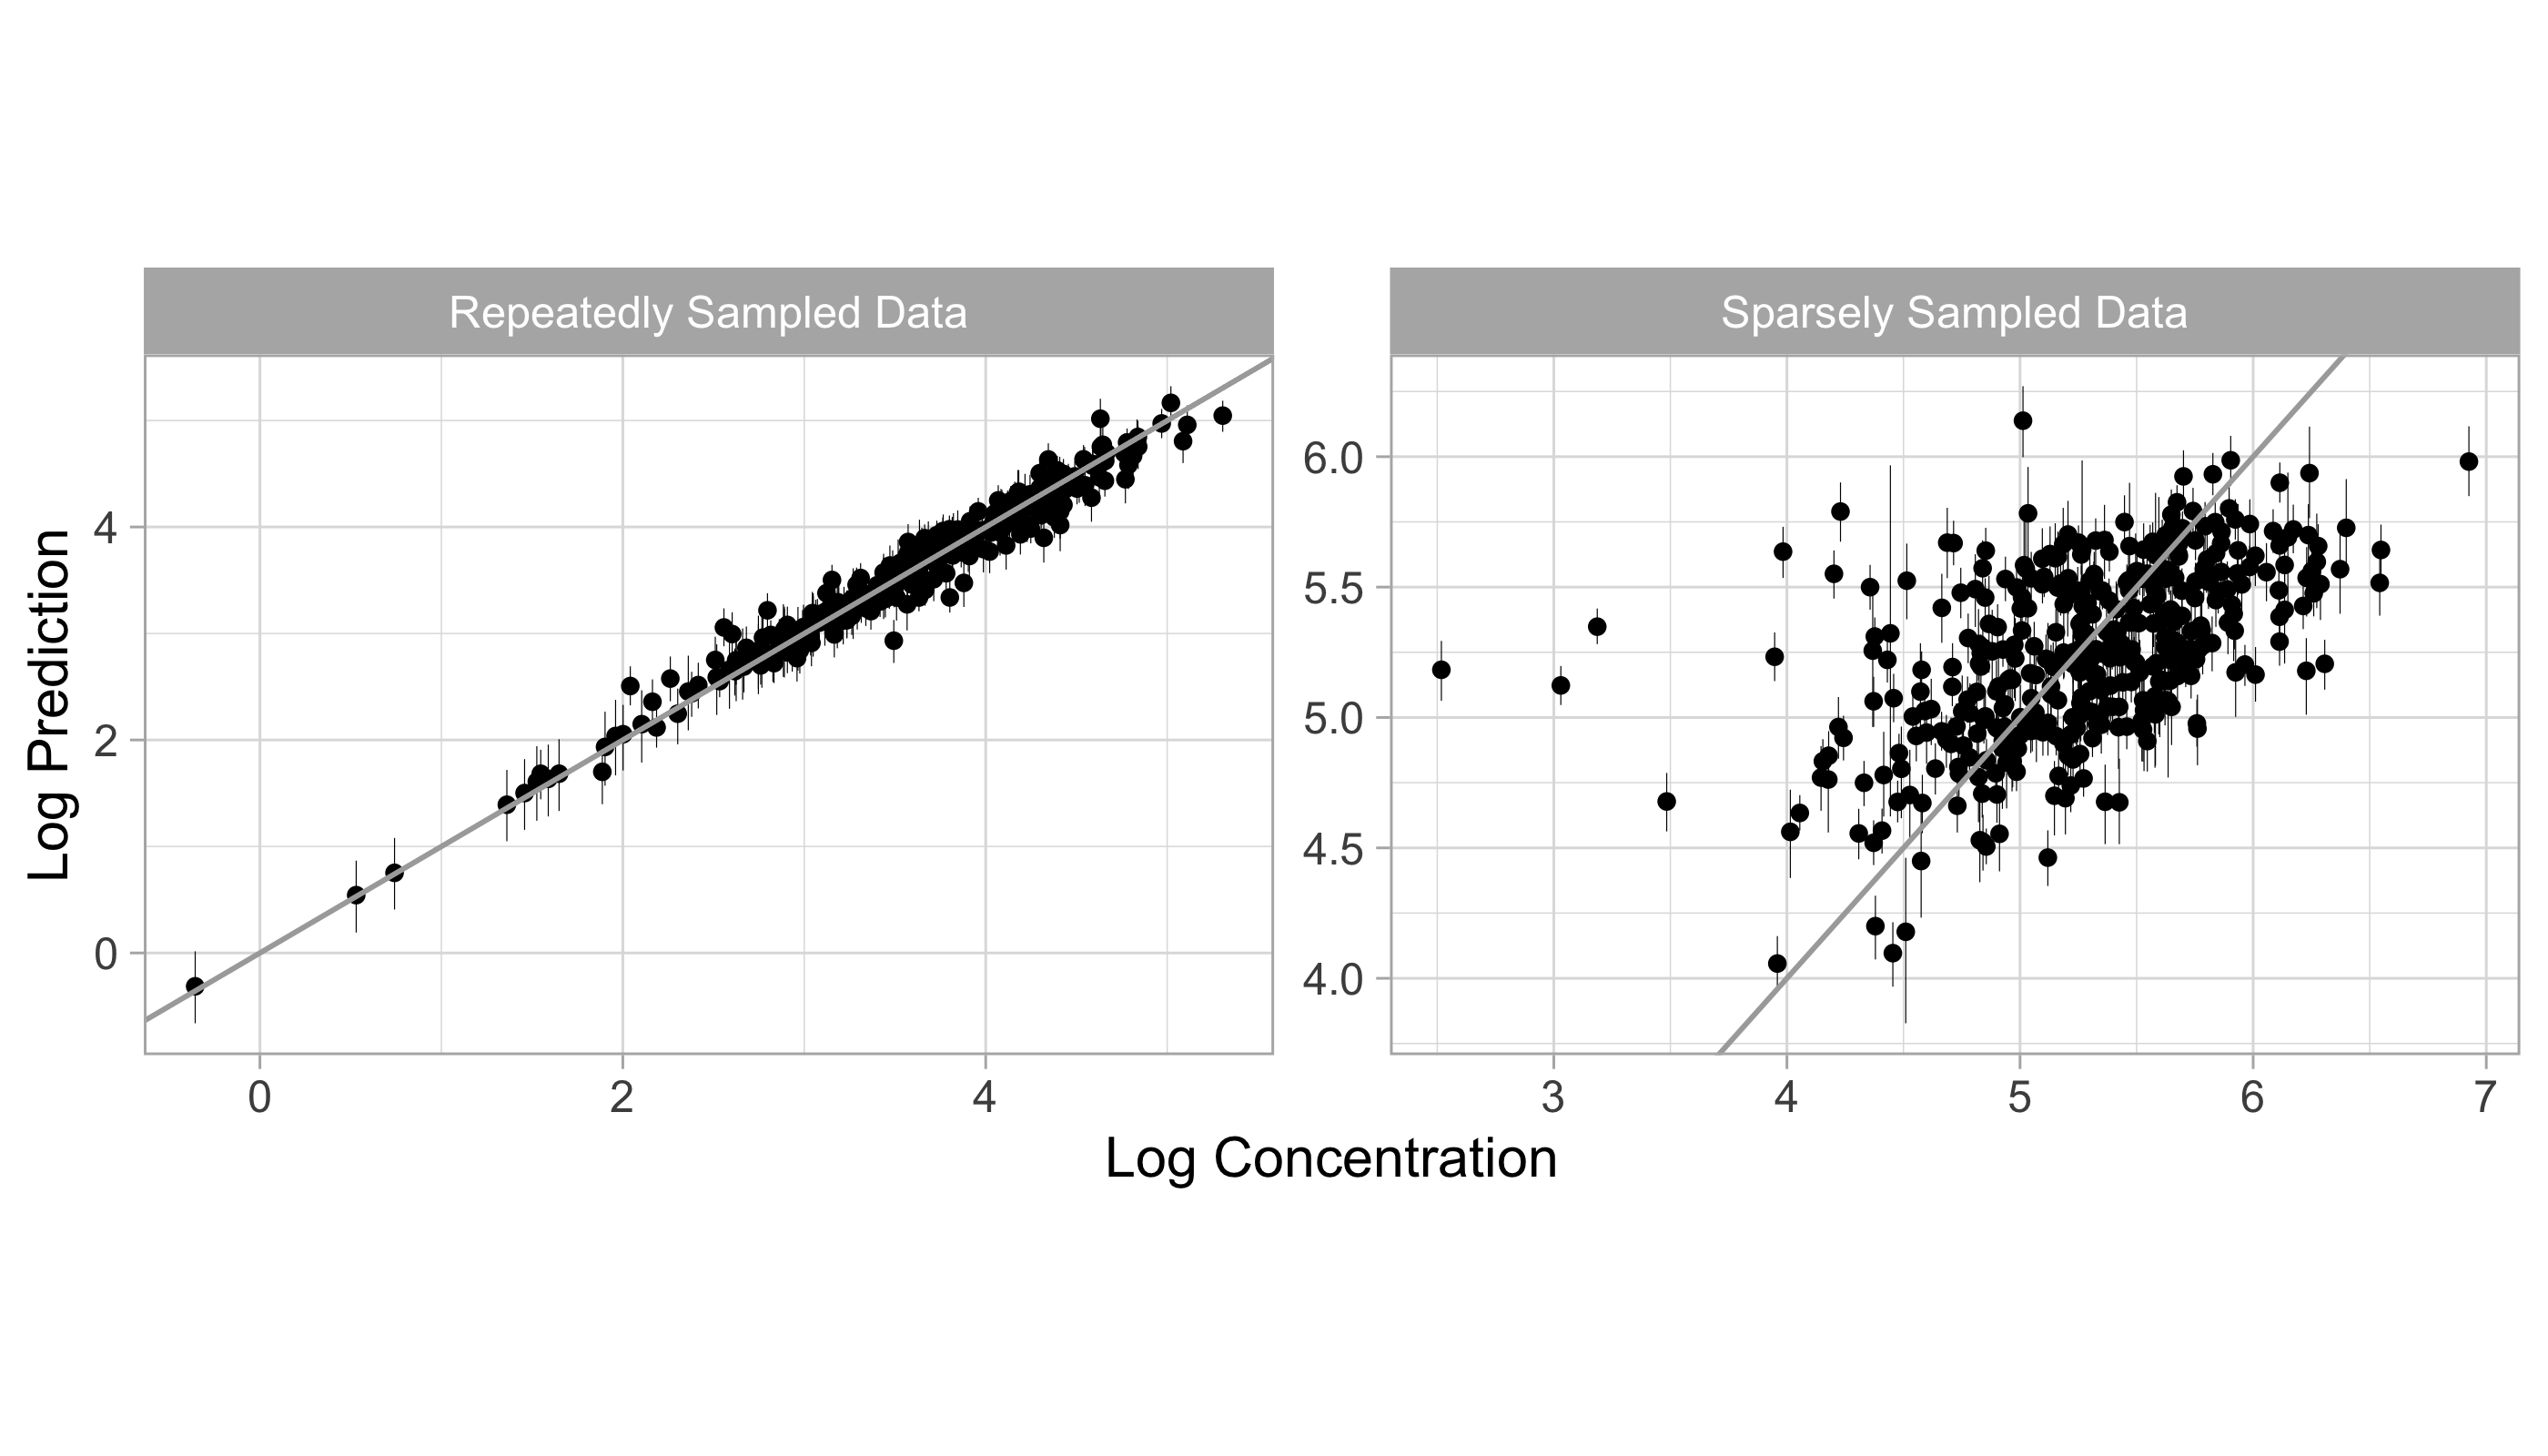
\includegraphics[width=\linewidth]{figures/plot-model-predictions-1} 
		
	}
	
	\caption{Predicted vs observed concentrations for both datasets on the log scale. Note each plot has a separate scale. Sparsely sampled data can not be predicted as accurately as the repeatedly sampled data, due in part to the inability to estimate patient random effects in pharmacokinetic parameters.  This additional variance left unexplained manifests as measurement error.}\label{fig:plot-model-predictions}
\end{figure}

\begin{figure}
	
	{\centering 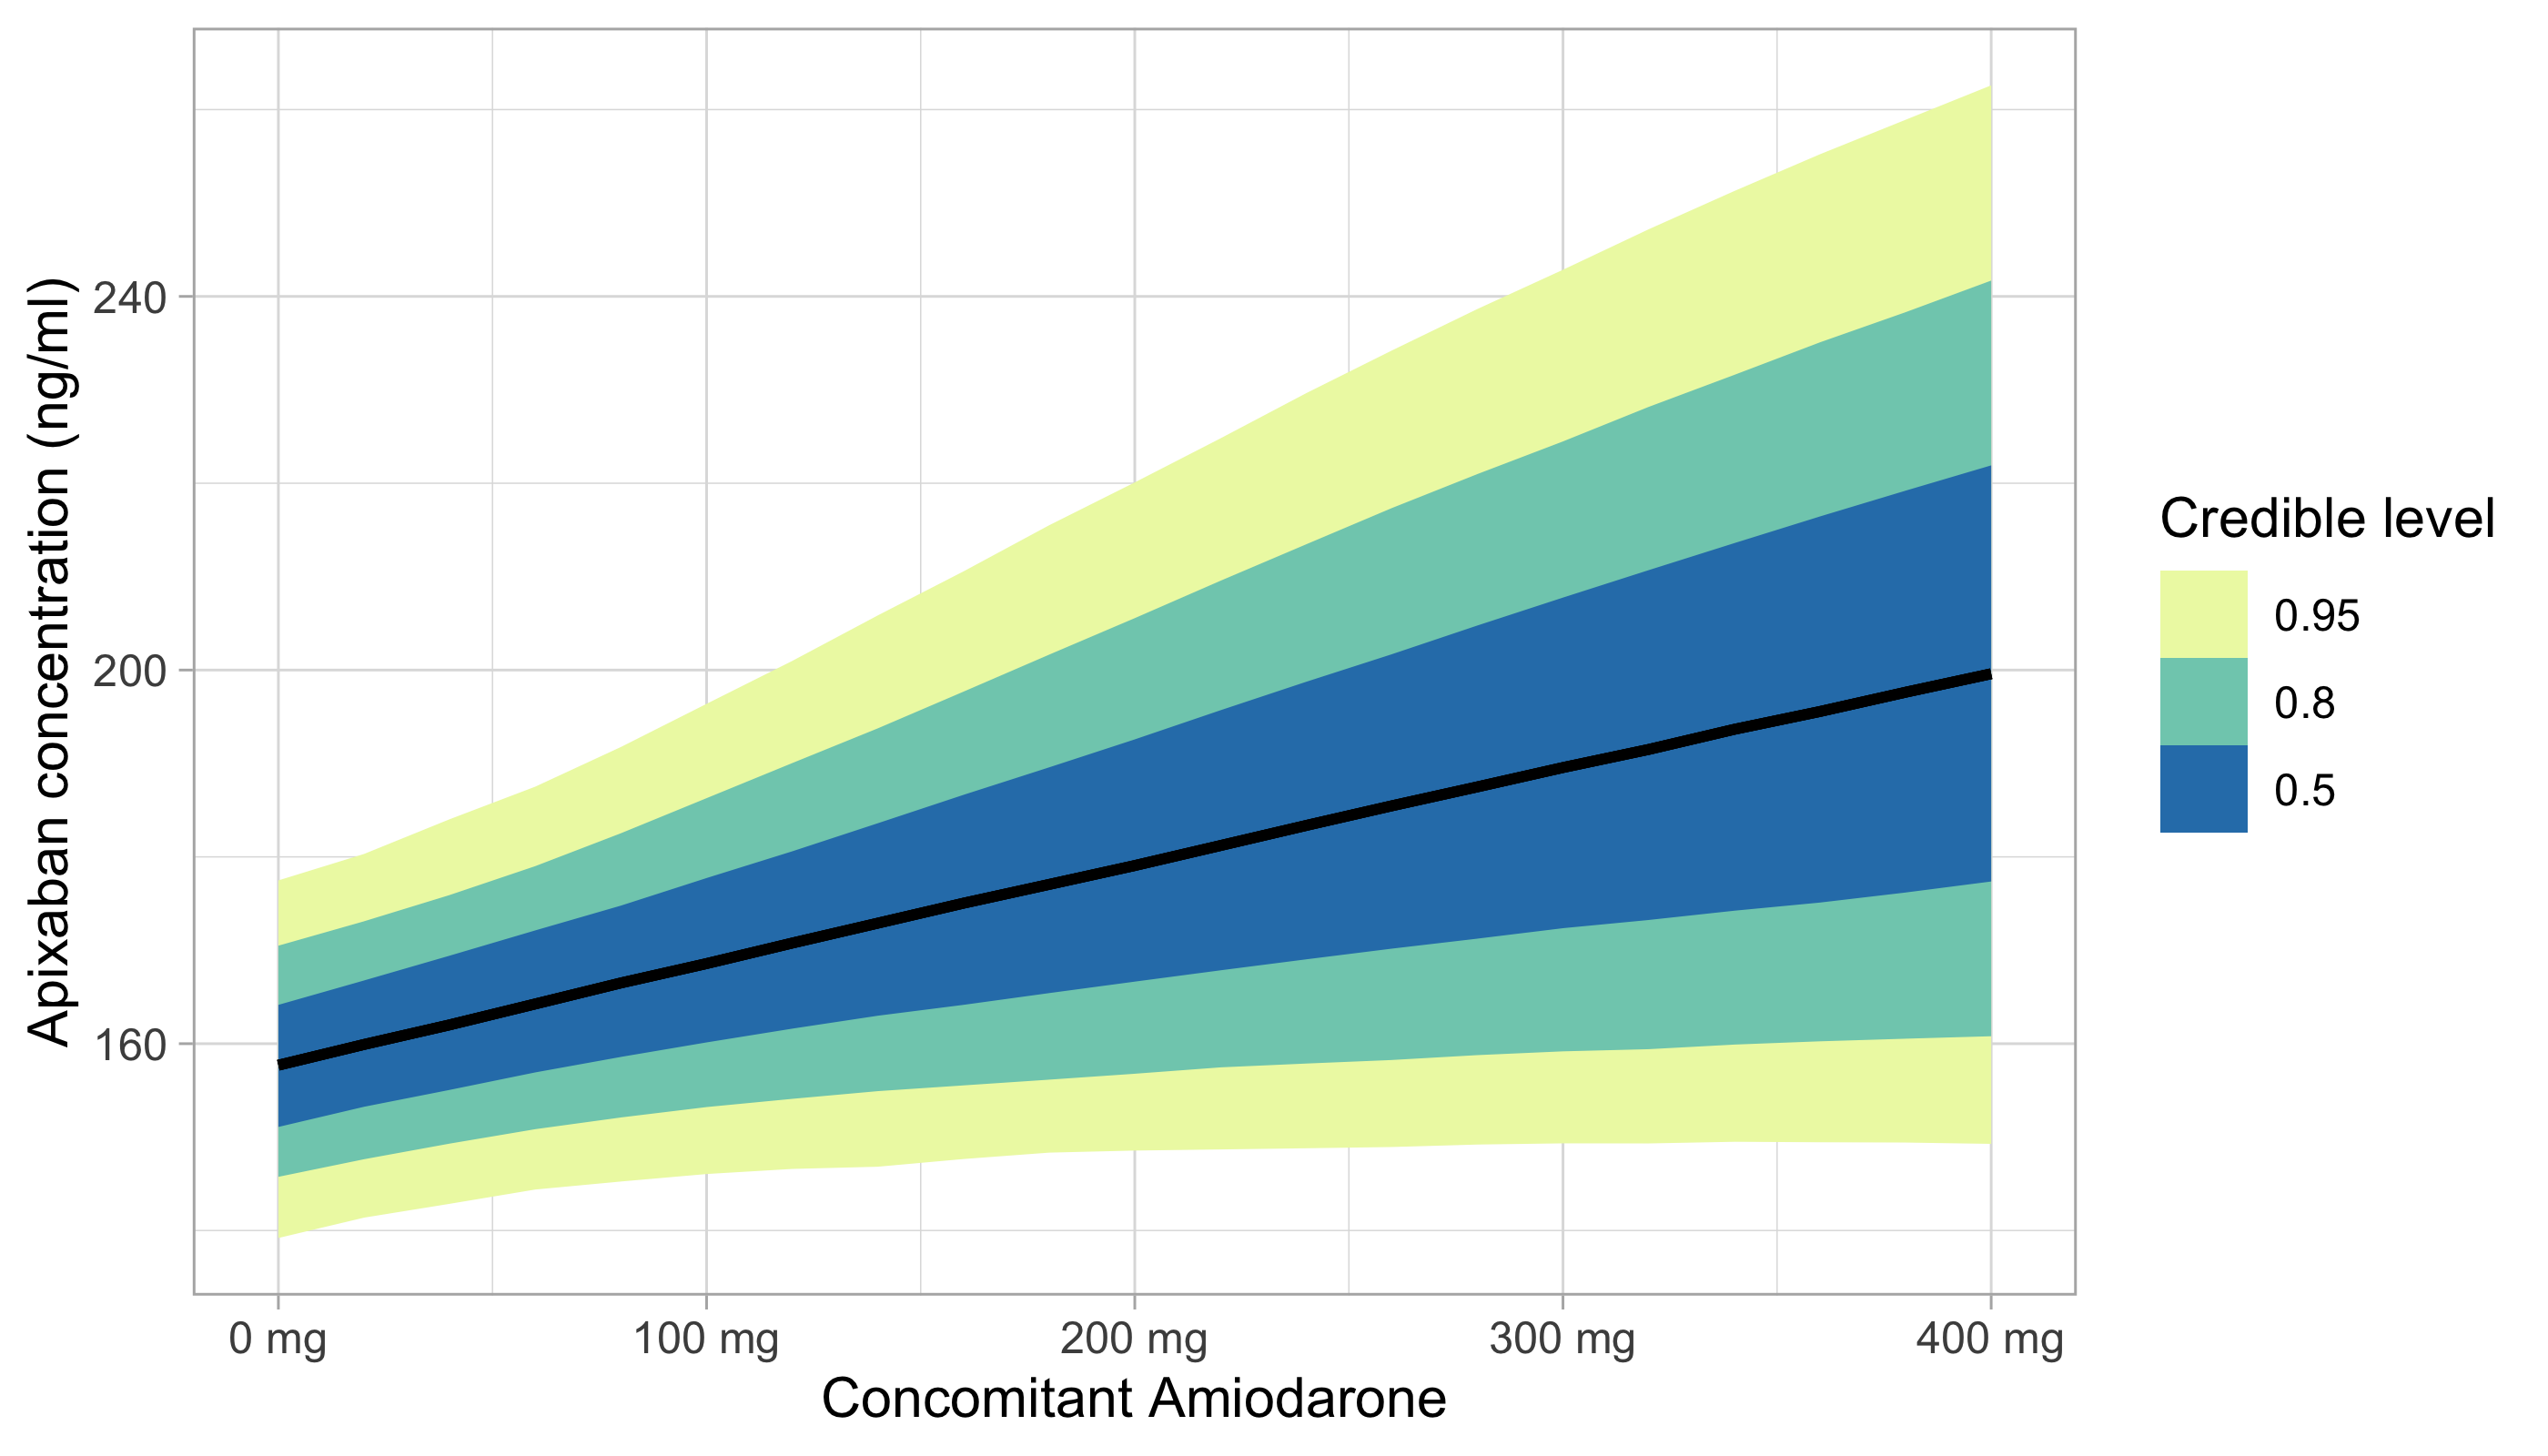
\includegraphics[width=\linewidth]{figures/max-concentration-1} 
		
	}
	
	\caption{Estimated max concentration as a function of concomitant amiodarone for a reference patient.  Concomitant amiodarone is estimated to increase apixaban bioavailability, thus leading to an increase in max concentration. The uncertainty in the effect of concomitant amiodarone is propagated through to the estimate of max concentration.  If max concentration is a key quantity in decision making, propagation of this uncertainty is crucial.}\label{fig:max-concentration}
\end{figure}

\begin{figure}
	
	{\centering 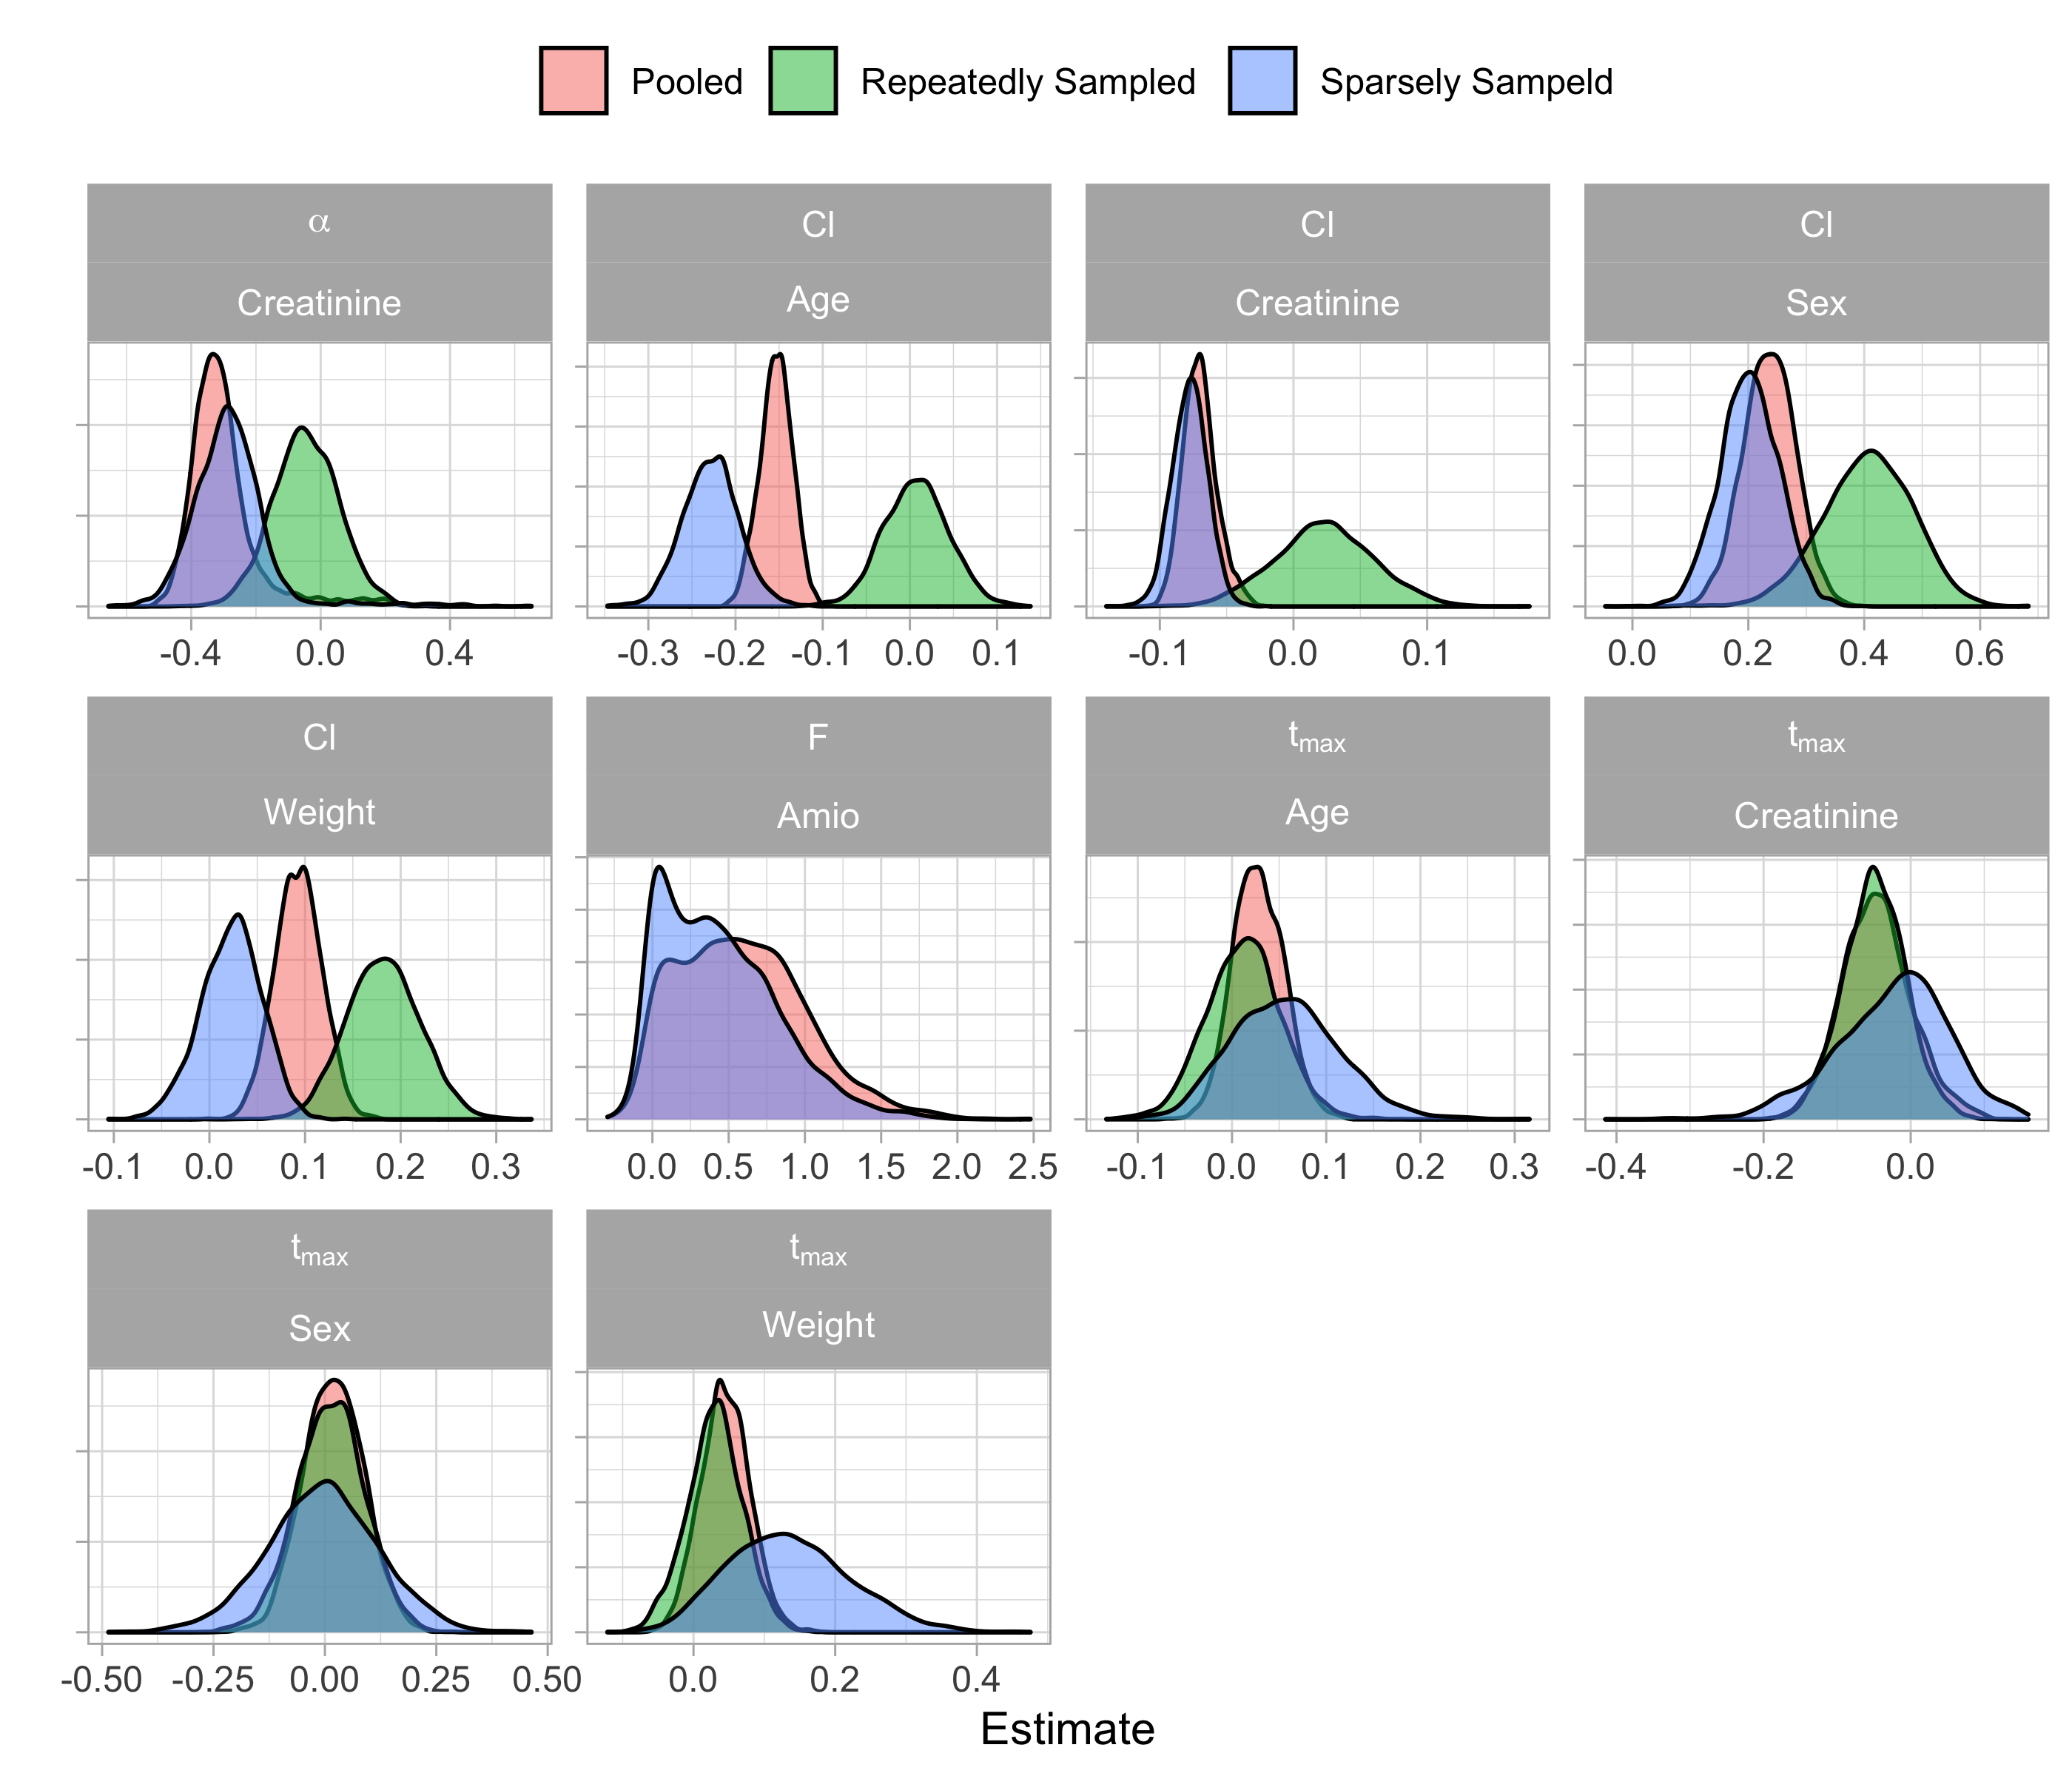
\includegraphics[width=\linewidth]{figures/effect-estimates-1} 
		
	}
	
	\caption{Estimated covariate effects from models fit to each dataset separately and the pooled model.}\label{fig:effect-estimates}
\end{figure}

		\section{Discussion}


The Bayesian model we present pools information across studies which may differ in study protocol.  Doing so allows investigators to make use of all available data -- be they from controlled studies, or arising from patient interactions in a personalized medicine clinic -- to fine tune pharmacokinetic models to populations of interest. However, this is just one possible model out of a family of similar models. One extension worth mentioning is estimating heterogeneity of effects between studies.  Our model assumes that for a given covariate, the effect is the same in different studies; the effect of weight on the clearance rate is the same across studies, for example.  This need not be assumed, and it may be the case that allowing for heterogeneity of effects between study populations may help explain additional variation beyond what measured covariates already explain.  The extension to include heterogeneity of effect is straightforward for our model, and would see an extended hierarchy considered where each $\beta$ and $\mu$ are generated from some further distribution with unknown parameters. We do not to implement this extension because our data consists of only two studies, making inference on the between study variability in effects difficult to estimate reliably.

To demonstrate how our model can be used to discover novel predictors of pharmacokientics, we included a simulation study in which we place a double exponential prior on a potentially novel covariate's effect on the bioavalability of the drug.  The double exponential prior acts as a sparsity inducing prior, pulling large effects towards 0 as the LASSO does. Our simulation study showed that our model is able to estimate the effect of this novel covariate reliably, even in circumstances where only a small amount of data on repeatedly sampled patients are available to investigators.  The estimates are biased towards the null due to the sparsity inducing prior. This bias attenuates with more data becoming available, and can also change depending on prior hyperparameters. From an estimation perspective, although the estimates of the effects are biased, they may be better suited to predict population effects due to this decrease in variability, similar to the phenomenon displayed by the James-Stein estimator \cite{stein1956inadmissibility,james1992estimation}.  We believe that since the primary goal of exploration is not to get very precise estimates, but to rather to discover new avenues for future research, the exchange of variance for bias is not only acceptable but also preferable.

Finally, we applied our model in a case study of apixaban.  We pooled data from two sources; one from a well controlled clinical study, and the other from an observational setting.  We used a sparsity inducing prior to regularize estimates of the effect of concomitant amiodarone on bioavailability of apixaban.  Concomitant amiodarone's effect on apixaban concentration has been previously studied \cite{gulilat2020drug}, however that model is more descriptive whereas our model is mechanistic (in so far as we model the pharmacokientics explicitly) and incorporates prior information from previous studies.  The findings in our case study and previous work agree; concomitant amiodarone is associated with an increase in apixaban concentrations. It is difficult to evaluate if the magnitudes are similar, however, mainly because our model posits a multiplicative effect whereas previous models assume an additive effect.  However, our model is capable of providing richer inferences due to the mechanistic model and fully Bayesian analysis.  We can propagate uncertainty in the effect of concomitant amiodarone through to other salient pharmacokinetic measures, like max concentration (see figure \ref{fig:max-concentration}).  Additionally, uncertainty in other pharmacokinetic measures can be propagated. For example, where as previous models relied on a point estimate of time to max concentration -- which was the same for each subject -- our model can estimate each patient's time to max concentration (conditioned on covariates) and uncertainty in that estimate propagates through to max concentration.  The posterior distribution of max concentration then captures all uncertainty relevant to the decision, meaning credible intervals should -- at least in theory -- also have better coverage for individuals.  Though a similar Bayesian pharmacokinetic model could be fit using only the sparsely sampled data, pooling information using repeatedly sampled data should be beneficial because of the high precision in estimates of covariate effects afforded by the repeated sampling.

The marginal posterior distributions of the effects display behavior consistent with partially pooled models.  Models fit to each dataset could be considered as a non-pooled estimate, our model -- which combines information from multiple datasets -- can be considered as a pooled estimate.  Partially pooled models have the effect of regularizing estimates towards the population mean, but the size of this regularization depends on the precision and magnitude of the estimate. This behavior is most clearly shown in the radon example provided in chapter 12 of Gelman and Hill's book on multilevel modelling \cite{gelman2006data}.  Gelman and Hill describe an analysis of exposure to radon -- a known carcinogen in high concentrations -- across 3000 counties in the United States.  Within each county, a variable number of houses were measured for radon exposure.  Importantly, some counties had more observations than others.  Within each county, an average level of radon exposure can be estimated.  However, those counties with fewer observations have smaller precision in the estimate.  Those counties with large effects and high precision see little regularization in the estimate of average radon exposure when comparing non-pooled estimates to pooled estimates.  Those counties with large effects and small precision see a strong amount of regularization (see figure 12.1 in  Gelman and Hill \cite{gelman2006data}). Similar explanations can be applied to our model.  As an example, we see that the effect of weight on clearance ($Cl$ in our model) has been regularized to be a compromise of the estimates obtained from models fit on the repeatedly and sparsely sampled data separately.  Additionally, we can see that there is little regularization in effects where one dataset provides a high precision estimate (as in creatinine's effect on clearance). The tendency for partially pooled models to regularize towards the population mean has the effect of trading variance for bias, a theme that has permeated this work.  This should in principle result in estimates of the effects with smaller root mean squared error.

Our study is not without limitations.  Firstly, our repeatedly sampled data come from a study concerning patients with Non-Alcoholic Fatty Liver Disease (NAFLD).  Some patients in this study had NAFLD, others did not.  Our sparsely sampled data did not collect this variable, and so technically it should be considered missing.  One strategy is to impute this variable, be it though frequentist methods or Bayesian methods.  We choose not to impute this and simply exclude it from our model since the study which generated the repeatedly sampled data failed to detect a statistically significant effect of NAFLD on apixaban pharmacokinetics \cite{tirona2018apixaban}. Additionally, because patients in the sparsely sampled data were sampled only once, we were forced to assume their time delay was 0.  The time delay is most probably non-zero, and making this assumption may increase the variability of estimates of other pharmacokientic measures.  Finally, the subjects in each study are quite different with subjects in the repeatedly sampled data being younger, healthier, and with better kidney function on average. Since subjects in the sparsely sampled data are generally different, a linear effect of covariates on pharmacokientic parameters may not be appropriate due to extrapolation.  A possible remedy for this would be to model the effects of covariates using splines or other suitably flexible methods.  If additional subject matter expertise is available, investigators may choose to model the effects with monotone-splines.  We believe specifications about the functional form of effects are best done with the aid of subject matter experts (pharmacologists, physicians, etc) and opt for the simplest non-trivial functional form for our effects.

\section{Conclusion}


In this study, we demonstrated how investigators could accomplish the goals of accurate modelling of pharmacokientics and exploration of new variables via the use of a heirarchical Bayesian model of pharmacokientics. The model pools information from multiple studies and shrinks estimates of effects.  The result is a trade off of variance for bias, which should improve predictive accuracy.  Additioanlly, we peformed a simulation study to demonstrate how sparisty inducing priors can be used to indentify effects of new variables.  We showed that, even in small samples, a small amount of bias is observed in estimates of novel effects and this bias attenuates with more data. Future research may include modelling heterogeneity of effect by adding another level to the hierarchy.
		
\chapter{Discussion}

This thesis has provided contributions towards the goals of identifying factors driving between patient variability in drug response, and selecting the optimal dose for a patient.  These problems were approached from the context of pharmacokinetics, arguing that drivers of variability in concentrations may be drivers of variability in response since concentration is a proxy for systematic exposure.  The first article presented a comparison of a population pharmacokinetic model fit using Maximum A Posteriori and Hamiltonian Monte Carlo for the purposes of decision making on dosing.  Additionally, a one compartment pharmacokinetic model with first order elimination was presented which leveraged a non-dimensionalization to force identifiability of the model and facilitated use of Hamiltonian Monte Carlo for sampling from the posterior distribution. The simulation studies from this article provided evidence that models fit using Hamiltonian Monte Carlo resulted in better calibrated decisions when the goal is to select a dose to avoid the risk of exceeding some concentration threshold.  The second article provided a framework for combining Bayesian pharmacokinetic models with dynamic treatment regimes for the comparison of various modes of personalization.  A case study on apixaban was used demonstrate the benefits of various forms of personalization and motivated conversation on if the benefits would outweigh the burden placed on the patient to adhere to additional follow up. The final article highlighted important violations of assumptions of exchangeability when combining data from different studies and offered a model which satisfies those assumptions, allowing investigators to combine all data available to them to perform inference on pharmacokinetic models. Sparsity inducing priors were also motivated as a means of determining if novel variables have an appreciable affect on pharmacokinetic measures, such as the drug bio availability. The sparsity inducing priors approach trades off variance for a small amount of bias and side steps issues associated with variable selection, a common approach used in determining which variables to include in a pharmacokinetic model.

\section{Key Themes}

\subsection{Paper 1}
New advancements in statistical theory can take time to be adopted across disciplines. In the case of HMC, theoretical understanding is still nascent, but additional theoretical and applied evidence for preferring HMC over MAP continues to mount.  Though theoretical warnings for MAP's deficiency were published earlier this decade, the first article in this thesis demonstrated that deficiency could manifest in non-obvious ways for models important to personalized medicine.  Indeed, models fit by HMC and MAP appeared to be equivalent when compared on predictive accuracy, but decisions made therefrom were very different with different outcomes.  MAP is motivated by low dimensional intuition --- that because integrals are linear operators, and density is largest around the mode, then the areas around the mode should contribute most to expectations.  The importance of intuition in statistics, and mathematical modelling of any kind more broadly, can not be over stated.  However, that intuition can fail in spectacular ways when dimensionality increases due to the so called ``Curse of Dimensionality''.

The shift from ``low'' dimensionality where intuition is effective to ``high'' dimensionality happens quickly. Modelling intuition needs to be validated, and that validation may not necessarily come directly from examining the fitted model (e.g. by examining the distribution of residuals).  The importance of simulating fake data and fitting proposed models to that data is a known but often unreported approach to model validation.  This approach may not be necessary for all techniques (for example when models are fit via optimization and the objective function is convex with unique optima, such in the case of most generalized linear models), but for non-standard models or models which are highly non-linear, it can be an effective tool for discovering hidden modelling pathologies.  Since the publication of the first article, additional research has been published on a ``Bayesian workflow''  \cite{gelman_bayesian_2020} in which fitting models to simulated data is listed as an explicit step.  Often, the inferences we wish to make go beyond that of parameter values, and fake data simulation can help in ensuring that the resulting model is capable of returning accurate inferences, or discovering that the model as written is incapable of doing so.

Additionally, fake data simulation can provide evidence that the model may not be able to be fit as it is written.  While HMC is effective and efficient, modelling benefits do not come for free.  When models suffer from pathologies detectable from sampling diagnostics, the remedies to those pathologies can be non-trivial. A naive implementation of the model presented in the first article suffered from slow sampling times, and often chains failed to converge to the same target distribution.  Often, the key to an effective implementation comes down to an effective parameterization, and this was the case for this model.  The non-dimensionalization offered a way to force identifiability of the model, and the result was an efficient sampling with no detectable pathologies.

\subsection{Paper 2}

Sequential decision making is an important aspect of personalized medicine.  However, there are sometimes in which sequential optimization is important, and others when it makes a negligible difference.  The second article in this thesis  provided a framework for evaluating different modes of personalization.  In that article, sequentially optimal modes of personalization yielded smaller regret on average than those which only used information from a single point in time.  However, the magnitude of that difference --- at least in the case studies presented --- were small.  The decision to implement one mode of personalization over another would thus also need to consider costs (monetary or otherwise) associated with each mode. While the considerations for those decisions may vary from facility to facility, statistical methodology can help to determine how much better one mode could perform over another \textit{in ideal circumstances}.

I don't know, something something something.

\subsection{Paper 3}

The observation that some drugs have variability in concentrations in excess of that observed in clinical trials motivates the ``fine tuning'' of pharmacokinetic models to a population of interest.  However, the data resources available to pharmaceutical companies may not be realistic for individual researchers or smaller institutions to obtain.  Making use of data collected on the same drug in different studies is one way to increase the data available for personalization.  The development of new methodologies and models to facilitate this combination is crucial, as the models will likely have to account for individual study peculiarities. Those developments can not happen in isolation and will require a collaboration between modellers and domain experts.

Investigators seeking to develop such new methods must be careful not to make simplifying assumptions which may threaten the internal validity of the inference. Previous models studying the effects of various clinical factors on apixaban concentration were perhaps \textit{too simple}\footnote{I feel comfortable saying this because \textit{I} was the one who recommended the approach \cite{gulilat_drug_2020}}.  The resulting inferences may have been valid from a statistical perspective, but could lack useful interpretation in the applied domain depending on which questions are being asked of the model.  This provides an extreme example, and future research would likely be subject to more nuanced challenges, such as the violation of exchangeability discussed in the third article. Carefully navigating the modelling process will require collaboration with expert modellers.  Those modellers must also be receptive to receiving feedback from domain experts, and must work diligently to extract necessary information from those experts.


\subsection{Future Work}

The foundation of this work is the Bayesian pharmacokinetic model, hence additional effort should be put into ensuring the model is of sufficient quality and aligns with expert knowledge.  In particular, ensuring the priors reflect expert knowledge as accurately as possible is a clear avenue for improvement.  This work could take many forms, including a Bayesian meta analysis to synthesize effects from various previous studies.  Additionally, the problem of prior elicitation from experts has spurred research in human computer interaction, resulting in interactive ways of evaluating the agreement of priors with expert knowledge \cite{sarma2020prior}.  Once priors are agreed upon, the construction of a Bayesian model from the population of interest can be performed.  This thesis leveraged data from highly controlled clinical study for most modelling efforts.  A more heterogeneous sample may lead to better generalizability, and hence better decisions made from said model.  Further work could be done to refine inferences from the measurement process too.  If instruments are calibrated, using data from the calibration process can provide useful information usable by the model.

The work presented in this thesis surrounding optimal sequential decision making used a value function which was simple and easy to interpret.  In reality, the value function used implicitly in the clinic is more complex and likely varies between clinicians.  The dosing decisions made by clinicians offer the opportunity to learn the implied value function and then use that value function in a dynamic treatment regime.  Additionally, there is the opportunity to explicitly incorporate health economic factors into the  framework presented here for purposes of comparing modes of personalization.

When combining data from different studies, it may be unlikely that all studies measure the same variables.  Work on Bayesian inference for missing variables could be used to extend the work I presented in the third article.  Additionally, while the variables from well controlled studies are likely high precision, those variables obtained from studies with less precision may benefit from an ``error in variables approach''.  These approaches will undoubtedly add uncertainty to the model, but honest uncertainty is likely preferable to exaggerated precision.

\section{Conclusion}

This thesis presented techniques for identifying factors driving variation in drug response and optimal dose selection using Bayesian statistics and dynamic treatment regimes in conjunction with pharmacokinetic models.  The methodologies presented here evaluated 




%% This adds a line for the Bibliography in the Table of Contents.
\addcontentsline{toc}{chapter}{Bibliography}
%% ***   Set the bibliography style.   ***
\bibliographystyle{plain} % (change according to your preference)
%%% ***   Set the bibliography file.   ***
\bibliography{bibliographies/thesis_bib}
%% ***   NOTE   ***
%% If you don't use bibliography files, comment out the previous line
%% and use \begin{thebibliography}...\end{thebibliography}.  (In that
%% case, you should probably put the bibliography in a separate file
%% and \include or \input it here).

%Appendices.
\begin{appendices}
% As ab example...
%\include{appendixa}
\end{appendices}

%CV only relevant stuff... not full CV.
\addcontentsline{toc}{chapter}{Curriculum Vitae}
\chapter*{Curriculum Vitae}
\begin{table}[ht]
\begin{tabular}{ll}
\textbf{Name:} & \firstname{} \lastname\\\\
\textbf{Post-Secondary} & La La School\\
\textbf{Education and}& La La Land\\
\textbf{Degrees:}& 1996 - 2000 M.A.\\\\
& University of Western Ontario\\
& London, ON\\
& 2008 - 2012 Ph.D.\\\\
\textbf{Honours and}& NSERC PGS M\\
\textbf{Awards:}& 2006-2007\\\\
\textbf{Related Work}& Teaching Assistant\\
\textbf{Experience:}& The University of Western Ontario\\
& 2008 - 2012\\
\end{tabular}
\end{table}
\subsubsection*{Publications:}
La La
\end{document}

